\documentclass{article}
\usepackage{titling}
\usepackage[margin=1in]{geometry}
\usepackage{multicol}
\usepackage{longtable}
\usepackage{amsmath}
\usepackage{amssymb}
\usepackage{booktabs}
\usepackage{graphicx}
\usepackage{makecell}
\usepackage{placeins}
\usepackage{lscape}
\usepackage{tabularx}
\usepackage{caption}
\usepackage{multirow}
\usepackage{subcaption}
\usepackage{times}
\usepackage{listings}
\usepackage[utf8]{inputenc}
\newcolumntype{Y}{>{\raggedleft\arraybackslash}X}
\newcolumntype{Z}{>{\centering\arraybackslash}X}
\newcolumntype{S}{>{\hsize=0.45\hsize}Z}
\newcolumntype{H}{>{\setbox0=\hbox\bgroup}c<{\egroup}@{}}

\usepackage{xcolor}

\usepackage{silence}
\WarningFilter{latex}{Text page}

\usepackage{url}
\usepackage{tikz}
\usetikzlibrary{arrows,angles,quotes,patterns,shapes.geometric}
\tikzstyle{startstop} = [rectangle, rounded corners, minimum width=3cm, minimum height=1cm,text centered, text width=6cm, draw=black, fill=red!30]
\tikzstyle{process} = [rectangle, minimum width=3cm, minimum height=1cm, text centered, text width=6cm, draw=black, fill=orange!30]
\tikzstyle{arrow} = [thick,->,>=stealth]

\setlength{\parindent}{20pt}
\setlength{\parskip}{0em}
\usepackage{setspace}
\linespread{1.5}

\usepackage{natbib}
\usepackage{bm}
\setcitestyle{authoryear,open={(},close={)}}

\makeatletter
\newread\pin@file
\newcounter{pinlineno}
\newcommand\pin@accu{}
\newcommand\pin@ext{pintmp}
% inputs #3, selecting only lines #1 to #2 (inclusive)
\newcommand*\partialinput [3] {%
  \IfFileExists{#3}{%
    \openin\pin@file #3
    % skip lines 1 to #1 (exclusive)
    \setcounter{pinlineno}{1}
    \@whilenum\value{pinlineno}<#1 \do{%
      \read\pin@file to\pin@line
      \stepcounter{pinlineno}%
    }
    % prepare reading lines #1 to #2 inclusive
    \addtocounter{pinlineno}{-1}
    \let\pin@accu\empty
    \begingroup
    \endlinechar\newlinechar
    \@whilenum\value{pinlineno}<#2 \do{%
      % use safe catcodes provided by e-TeX's \readline
      \readline\pin@file to\pin@line
      \edef\pin@accu{\pin@accu\pin@line}%
      \stepcounter{pinlineno}%
    }
    \closein\pin@file
    \expandafter\endgroup
    \scantokens\expandafter{\pin@accu}%
  }{%
    \errmessage{File `#3' doesn't exist!}%
  }%
}
\makeatother

\newcommand{\rot}[2]{\rule{1em}{0pt}%
\makebox[0cm][c]{\rotatebox{#1}{\ #2}}}

% Specify formatting for displaying code blocks 
\definecolor{codegreen}{rgb}{0,0.6,0}
\definecolor{codegray}{rgb}{0.5,0.5,0.5}
\definecolor{codepurple}{rgb}{0.58,0,0.82}
\definecolor{backcolour}{rgb}{0.95,0.95,0.92}

\lstdefinestyle{mystyle}{
    backgroundcolor=\color{backcolour},   
    commentstyle=\color{codegreen},
    keywordstyle=\color{magenta},
    numberstyle=\tiny\color{codegray},
    stringstyle=\color{codepurple},
    basicstyle=\ttfamily\footnotesize,
    breakatwhitespace=false,         
    breaklines=true,                 
    captionpos=b,                    
    keepspaces=true,                 
    numbers=left,                    
    numbersep=5pt,                  
    showspaces=false,                
    showstringspaces=false,
    showtabs=false,                  
    tabsize=2
}

\lstset{style=mystyle}


\title{\large \textbf{Using Satellites and Phones to Evaluate and Promote Agricultural Technology Adoption: \\ Evidence from Smallholder Farms in India}
\thanks{We gratefully acknowledge financial support from ATAI and HBS’ Division of Research and Faculty Development. We thank Claudia Carbajal Morelos and Arnesh Chowdhury for superb research management and support, Jaagruti Didwania, Azfar Karim, and Prathyush Parasuraman for excellent research assistance, Tarun Pokiya for his agricultural expertise and suggestions, and the PAD India team for implementation support. 
Disclosure: Shawn Cole is a board member of Precision Agriculture for Development (PAD), an NGO specializing in delivering mobile phone-based extension to small-holder farmers. Cole does not receive any financial compensation from the organization. Harigaya is, and Killeen and Krishna were, employed by PAD. Cole: \texttt{scole@hbs.edu}; Harigaya: \texttt{tharigaya@precisionag.org}; Killeen: \texttt{gkilleen@berkeley.edu}, Krishna: \texttt{akrishna@gmail.com}}}

\begin{multicols}{2}
\author{
    Shawn Cole\\
    Harvard Business School\\
    \\[-0.5em] 
    Grady Killeen \\
    University of California, Berkeley \\
  \and
    Tomoko Harigaya\\
    Precision Agriculture for Development\\
    \\[-0.5em] 
    Aparna Krishna \\
    Indian Institute of Technology, Dhanbad
}

%\author{Shawn Cole \\[-0.5em] Harvard Business School \\ \\[-0.5em] Tomoko Harigaya \\[-0.5em] Precision Agriculture for Development \\ \\[-0.5em] Grady Killeen \\[-0.5em] University of California, Berkeley \\ \\[-0.5em] Aparna Krishna \\[-0.5em] Indian Institute of Technology, Dhanbad}

\date{June 2021}
\end{multicols}

\begin{document}

\tolerance=20000
\hbadness=20000
\vbadness=20000


\begin{titlepage}

\maketitle
\thispagestyle{empty}
    \begin{abstract}
        \singlespace
      Satellite data can measure smallholder farmer yields cheaply, yet is not widely adopted, especially in RCTs. We use an experiment to estimate the impact of a low-cost, customized soil nutrient management advisory in India. Satellite data provide more precise point estimates than survey data. Power gains (expressed as a reduction in required sample size) obtained from more accurate measurements (68\%), lower attrition (15\%), and the ability to include more years of baseline data (17\%) reduce the sample size needed to detect a five percent increase in yields by 77\%; and over 90\%  if there is differential attrition. We provide a non-technical “cookbook” with code for other researchers to easily measure yields with satellite data.While the intervention affects fertilizer usage, we do not find any gains in yields. The experiment demonstrates the potential to improve agronomic knowledge linking advice to output in a low-cost manner.
    \end{abstract}
\end{titlepage}

\section{Introduction}

Information technology has transformed farming in the developed world. Precision farming - farm management informed by increasingly data-driven, dynamic, and accurate instructions - has been credited with raising profitability by as much as 3\% \citep{Schimmelpfennig2016FarmAgriculture}. The dramatic reduction in costs of collecting and disseminating information in developing countries offers the tantalizing prospect that such approaches may improve productivity among small-holder farmers as well. This paper evaluates how such an approach might be adapted, in the setting of India, evaluating the ability of satellites to measure small-holder yields within the context of a field experiment; and testing whether mobile phones can be used to deliver advice which is trusted and acted upon. 

We designed an experiment to test the effect of customized fertilizer recommendations on fertilizer adoption and usage among cotton farmers in Gujarat, India, and evaluate our ability to measure yields. The sample for this experiment consists of 1,585 farmers who had recently signed up for a mobile phone-based agricultural advisory service, called Krishi Tarang (KT)\footnote{KT service is provided by Precision Agriculture for Development (PAD).}. The KT service provides comprehensive farming advice (on sowing, weeding, pesticides, harvesting, etc.) via automated voice messages throughout a cropping cycle. We randomly selected half of these farmers to receive plot-level soil fertility information and customized recommendations on three of the most common macronutrients and one micronutrient fertilizer (Zinc). These recommendations were delivered in a scalable manner: through the distribution of written information (Soil Health Cards and supplemental materials) prior to sowing, and a series of appropriately timed automated push calls during the growing season. To measure yields, we use both in-person surveys and satellite images. While remote sensing does require the mapping of individual plots, such mapping need not be done at the start of the experiment, and may potentially be useful for evaluating outcomes of interventions in settings where in-person surveying is difficult or expensive.

We find that satellites can effectively measure small-holder yields, even in a setting where our initial experiment did not anticipate their use. The power gains to evaluating the intervention are dramatic, and suggests that other evaluations of agricultural interventions may benefit from using remote sensing data. Our application within the context of a field experiment allows us to document ``real world'' gains from the use of satellites. Power gains (expressed as a reduction in required sample size) are obtained from three primary sources. First, simply collecting less noisy (more accurate) measurements would reduce the necessary sample size by 68\%. Second, satellites enable econometricians to control for multiple years of pre-data, which can be particularly important when rainfall patterns vary from year to year. Using one and two years of pre-intervention data reduces the sample size by 7 and 22\% compared to an approach using only ``post'' data -- and in fact, in our setting, because aggregate rainfall varies from year to year, the best predictor of yields in our experimental year is yields from two years prior. Third, attrition using satellite data is quite low -- 99.8\% of mapped plots in our sample appear in the data in all three years we consider. However, the biggest potential power gains come from eliminating the chance of differential attrition; not using Lee bounds, for example, reduces the necessary sample size by 73\%. Taken together, an experiment with satellite yields requires a 77\% smaller sample (ignoring attrition concerns), or an astounding 92\% decrease using (admittedly conservative) Lee bounds with missing farmer-reported data.

With respect to farmer behaviour change and yields, the evidence is more mixed. Both treatment and control farmers received general agricultural advice via mobile phone. The treatment group received additional advice on nutrient management, and most farmers listened to messages. We find changes in self-reported fertilizer usage that are large within the context of the literature, but small relative to potential yield gains. Furthermore, neither noisy self-reported yields nor satellite data detect any yield gains from the intervention, perhaps in part because rainfall was particularly poor in our intervention year.

Returns to fertilizers are highly sensitive to dosage and heterogeneous by local conditions \citep{Duflo2008HowKenya,Suri2011SELECTIONADOPTION}, and governments in many countries are seeking to promote site-specific nutrient management. For example, since the launch of the Soil Health Card (SHC) scheme in 2015, the Indian government reports having conducted at least 50 million soil tests and delivered over 200 million SHCs with plot-specific fertilizer recommendations. Evidence suggests that Site-Specific Nutrient Management (SSNM), formed on the basis of these four principles, can lead to enhanced yields and improved soil quality under controlled environment \citep{Khurana2007PerformanceIndia,Pampolino2007EnvironmentalSystems,Cassman2002AgroecosystemsManagement,Matson1998IntegrationManagement}, though there is a paucity of literature examining whether locally-specific advice on fertilizer dosage and usage would lead to similar results in real-world, small-holder settings. ICT may be particularly well suited to improve the ‘rate, timing, source and placement’ of fertilizer, which could enhance effectiveness of fertilizer application on plant absorption \citep{Pagani2013Site-SpecificReturn}.

This paper makes contributions to two literatures, (i) the use of remote sensing, particularly in experiments, and (ii) the promotion of agricultural technologies, such as fertilizer. 

A recent body of research has demonstrated the potential of modern satellites to measure small-holder yields, and changes in yields, with greater accuracy than surveys. For instance, \citet{Lobell2019EyesAnalysis} compare full plot harvest data, crop cuts, satellite yield measurements, and farmer-reported yield data from small-holder maize plots in Uganda. They find that satellite yield measurements are about as accurate as crop cuts, and satellite data is substantially more predictive of true productivity than farmer-reported data. \citet{Jain2019TheData} show a high correlation between satellite wheat yield measurements and crop cuts in a split-plot experiment in India, and that satellite data performs well at measuring the effect of a fertilizer spreader. Satellites are thus able to accurately capture yield differentials in this setting. Our paper builds on existing work, by evaluating the performance of satellite productivity measurements in a randomized controlled trial, evaluating the power gains, and by providing a ``cookbook'' to make this approach accessible to a broad set of development researchers. In our sample, we show that the confidence interval of effect size using satellite data is about 55\% the size of the interval obtained from household surveys if differential attrition is ignored. Using Lee bounds, we show that satellite data usage offers a confidence interval 73\% smaller. While there is an additional cost associated with mapping GPS coordinates of the plots, this cost is small (\$3.20 per plot, in our setting), relative to the power gains. 

This paper builds on a large literature that seeks to evaluate agricultural extension. It is most closely related to \citet{Fishman2016CanBihar}, which evaluated providing in-person customized fertilizer advice in Bihar, India, but found that the advice did not affect the farmers' fertilizer application decisions. \citet{Fishman2016CanBihar} propose limited trust and limited comprehension as barriers; our intervention seeks to overcome both factors. 

We make three contributions related to agricultural extension. First, inspired by work on vaccines in Pakistan \citep{Usman2011RandomizedEducation}, we demonstrate that a human-centered design approach, emphasizing electronic delivery, generates more trust, and reported behavior changes, in a country where in-person visits have failed. In a ``lab in the field'' setting, \citet{Cole2017TheAgriculture} find that the majority of cotton farmers in their survey sample in Gujarat had difficulty understanding recommendations in a government SHC but that digital and non-digital aid materials significantly improved comprehension levels. This paper uses an intervention very similar to \citet{Cole2017TheAgriculture}, and demonstrates that farmers understand, trust, and report acting on customized advice. To our knowledge most literature on trust in digital information has focused on developed markets (e.g., \citet{Sillence2006AAdvice}, or \citet{Bonhard2006KnowingSystems}).

More generally, the paper contributes to a growing literature exploring how advice delivered via mobile phones can increase technology adoption and improve agricultural outcomes \citep{Casaburi2019HarnessingKenya,Fabregas2019SMS-extensionAfrica,Cole2020MobileizingSustainability}, and the literature on gains to fertilizer use more generally (e.g. \citet{Beaman2013ProfitabilityMali}). 

Finally, our study contributes to the literature on the possibility of using precision farming techniques in the developing world \citep{Mondal2009AdoptionStrategies,Maohua2001PossibleMillennium}. On a positive note, we demonstrate that relatively small samples can yield precise estimates of the impact of interventions, suggesting that this approach may help generate improved agronomic knowledge, and that agronomic knowledge may be transmitted back to farmers at low cost. However, the results also serve as a cautionary tale. Governments are increasingly investing resources to build databases on local conditions and farmer characteristics, with the goal of providing increasingly customized advice. Our findings suggest that further research is warranted to verify that the investment in soil health card mapping would bear fruit: while we find that farmers report changing behavior, we do not observe yield gains.  

\section{Background and Experimental Design}

While fertilizer use is widespread in India (over 75\% of cultivated land uses fertilizer\footnote{Input Survey, 2011}), farmers have limited access to advice about optimal quantities. For example, only 6\% of farmers reported interacting with an extension agent in the previous year \citep{Cole2017TheAgriculture}, and respondents in our baseline survey answered only 2.3 of six questions about fertilizer correctly.

To improve soil health management, the Government of India launched a Soil Health Card scheme in 2015, with the goal of testing soil at fine spatial resolution\footnote{2 x 2 hectare grid for irrigated farmland}, and delivering personalized SHC to every farmer in India (\url{https://soilhealth.dac.gov.in/}). However, \citet{Cole2017TheAgriculture} note potential shortcomings with the government's approach. Not all farmers may receive soil health cards. Moreover, the technical presentation of data is difficult to understand, and only 8\% of farmers in their sample in Gujarat understood the basic recommendations on the SHC. 

\subsection{Intervention}

This study was implemented in partnership with Precision Agriculture for Development (PAD), an NGO specialized in providing mobile phone-based agricultural extension service. PAD supports Krishi Tarang (KT), a two-way mobile phone-based agricultural advisory service. Farmers subscribed to the KT service receive weekly push calls with information on seeds,  pesticides, planting, harvesting, and other agricultural decisions. Farmers can also call back into the system to access their personal inbox, re-listen to the messages sent through push calls, and record any questions, which would be answered by a PAD agronomist within two days. The service is offered for free and currently has more than sixty-thousand active users, overwhelmingly growing cotton, across thirty-six districts of Gujarat, a state in western India. 

\citet{Cole2020MobileizingSustainability} evaluate an early version of the service, finding high demand for the service, and evidence of systematic changes in agricultural practices. An important potential advantage of ICT delivery advice is the ability to deliver individually customized advice. To examine the feasibility of such an approach, PAD designed a set of messages that explain the importance of soil fertility management and provided farmers with information on plot-level soil nutrient levels, benefits and recommended dosages of three macronutrient (UREA, DAP, MOP) and one micronutrient fertilizer (Zinc).\footnote{Only UREA was recommended for unirrigated cotton.}

The specific intervention we study is inspired by government campaigns to inform farmers about their soil health, but to offer additional supportive content. For all farmers in our study, PAD sent field staff to collect a soil sample from the farmer's primary cotton plot as part of the baseline survey; soil tests were performed by a local agricultural university; and PAD applied the university’s fertilizer model in combination with soil test results to generate fertilizer recommendations\footnote{Technical details of the process of generating fertilizer recommendations are summarized in \ref{t:fertilizer-recommendation-methodology}.} customized for the individual plot. 

While in theory PAD could have drawn information from mass soil tests conducted by the government, previous work \citep{Cole2017TheAgriculture} raised concerns about the accuracy of government soil tests.

Treated farmers received customized recommendations through multiple channels while control farmers did not receive soil health results during the study period. At the start of the agricultural season, PAD hand-delivered a Soil Health Card (SHC) and two supplementary, customized, printed materials to each treated farmer in our sample. To ensure that recommendations were understandable and actionable, we simplified the design of SHC using an iterative process of testing the comprehension level and tweaking the design based on feedback from farmers in the study area while maintaining the amount of information provided in the SHC (\ref{f:shc}).

In addition, supplemental materials were designed to help farmers understand the fertilizer recommendations: a card (\ref{f:shc_supplement}) that lays out the timing and the quantities of different fertilizers recommended without detailed information on nutrient values and a booklet (\ref{f:shc_booklet}) that provides pictorial illustration of the potential effects of each fertilizer type on plant health and yields.\footnote{As the spread of smartphones and data plans increases, we imagine these visual aids could be delivered in video format at low cost.}

Finally, appropriately timed recommendations on fertilizer application were delivered through push voice calls over three months between June and September, incorporated into PADs advisory service. Push calls were timed to coincide with key stages in the crop growth cycle. In each call, PAD announced the topic of the call (macronutrient fertilizers, MOP, or zinc fertilizers), specified whether the call was for irrigated or unirrigated cotton, explained the potential benefits of the fertilizer(s), and provided the recommended application quantities (recommendations were given in amount per area unit). If farmers did not pick up the call on a scheduled day, calls were sent again the day after. On both days PAD made three attempts to reach farmers if they did not pick up the call. The share of farmers that listened to the push call recommendations, presented in \ref{t:treatment-call-listening-rates}, was greater than 0.7 for every topic except for mid-season zinc application. 

\subsection{Sample frame}

The sample of this study consists of cotton farmers who registered into the KT service in the first quarter of 2018 across three districts (Surendranagar, Rajkot and Morbi) in the southwestern region of Gujarat. PAD administered a screening survey and identified farmers who owned a mobile phone, were planning to grow cotton in the upcoming Kharif season, and were interested in receiving agricultural information through the KT service but had not subscribed to the service before. The baseline sample, including all farmers who had a plot suitable for soil collection, was 1,585 farmers.\footnote{A soil sample could not be collected if there were standing crops from the previous season or if fertilizer had been applied after harvesting of the previous year’s crop.}

\subsection{Randomization and sample characteristics}

Farmers in the base sample were stratified by block (district subdivision) and randomly assigned to a treatment or control group (793 and 792 respectively). Table \ref{t:balance} presents summary statistics of the key variables at baseline by experimental groups. Column (1) reports the control group mean and standard deviation of these variables. The average age of farmers in the study was 43 years, over 95\% of the sample indicated that their primary occupation was self-employed farming, and more than eighty-percent of respondents were literate (could read a newspaper in the local language). The average farmer had a total cultivated land size of about 3.5 hectares the year prior to the intervention, slightly above the national average of 2.35 hectares among all cotton farmers in India. Even though the Indian government launched a nationwide Soil Health Card scheme in 2015 with the plan of conducting a soil test for every farmer, fewer than 15\% of farmers in our sample reported ever having their soil tested. The remainder of the table reports balance checks, for the randomization (Column 2), and for comparisons based on baseline characteristics among the sets of farmers who did not attrit in subsequent surveys: a basal survey (conducted a few days after PAD recommended applying the first application of fertilizer), a midline survey (conducted in October-December 2018), an endline survey (conducted in February-May 2019), and a separate plot mapping exercise (conducted in March-May 2019). The p-value of an F-test of the joint orthogonality of the variables is included at the bottom of Columns (2) - (7). 

Table \ref{t:balance} shows that the proportion of baseline variables imbalanced between the two experimental groups are below the corresponding significance levels, indicating that the two groups are well-balanced. We will discuss differential rates of attrition in Section \ref{t:sat-vs-fr-treatment-effects}.  In addition to the survey data, we obtain administrative data on KT service usage including pickup rates, and amount of time spent listening to messages. These data are available for both treatment and control groups, though only treatment groups received supplemental fertilizer advice. 

\subsection{Empirical strategy}

We estimate an ITT with OLS:
$$
Y_i = \alpha_b + \beta T_i + \epsilon_i
$$

where $Y_i$ denotes the post-intervention outcome for individual $i$, $T_i$ the treatment indicator, and $b$ the sub-district fixed effects.

One goal of this paper is to better understand whether and how point estimates and standard errors change depending on the methodology used to measure outcomes. To the extent possible, we seek to separately identify differences due to changes in sample composition vs. change in the noisiness of the measure. To that end, we report the results of several regressions across four samples. First, we present results across the full sample. Second, we present results across the sample of respondents that provided yield data. This sample size is equal to 1,341, which is 61 observations smaller than the set of respondents that completed the endline survey because some farmers did not provide productivity data during the survey. Third, we restrict the sample to the 1,326 respondents for which we have 2018 satellite yield data. Fourth, we examine the set of respondents for which farmer-reported and satellite yield data are available. 

\section{Results}

\subsection{Take-Up: Listening Rates of Customized Fertilizer calls}

Take-up of the information service, detailed in \ref{t:treatment-call-listening-rates}, was quite high, with 76\% (unirrigated) to 88\% (irrigated) of farmers picking up and listening to basal fertilizer recommendations. In fact, 50\% of the treated farmers listened to the same recommendation more than once. Pick-up rates were lower for calls later in the season, but the listening rates for all but one of the recommendations remained above 70\%. In total the average treatment farmer was exposed to 42 minutes of content on fertilizer application.

However, we observe some ``crowd out'' of information, as treated farmers are 3.5 percentage points less likely to pick up subsequent weekly calls on cotton farming advice (Table \ref{t:engagement-and-knowledge}), this difference is significant at the 1\% level. However, Column (2) shows that, unconditional on picking up, treatment farmers listened to approximately the same amount of total non-fertilizer content, meaning that the total exposure to content was roughly equivalent. 

The intervention appears to have increased trust in the KT service. Treated farmers rated non-fertilizer KT calls higher by an average of 0.148 points on a 5-point scale, and they were 3.3 percentage points more likely to report using a mobile phone-based advisory service to make agricultural decisions during the endline survey. The intervention also increased reported trust in mobile phone-based advisory by over 0.2 points on a 5-point scale ($p < .01$). 

\subsection{Impact on fertilizer knowledge}

Surveyors administered a 14 question multiple choice quiz about basic facts relating to fertilizer during the midline survey to measure whether the treatment increased farmers’ fertilizer knowledge (See \ref{t:knowledge-questions} for questions). Baseline knowledge was low, with farmers answering approximately 3.2 questions on average. The intervention increased fertilizer knowledge: farmers in the treatment group provided the correct response to 0.266 - .316 more questions, depending on the exact sample. The knowledge gains are statistically significant at the 1\% level across all samples. Taken together, the high adoption of the customized fertilizer recommendations, increased trust in mobile phone-based advisory, and improved fertilizer knowledge indicate that trust and comprehension of the fertilizer recommendations was high. The intervention was thus able to alleviate some of the information frictions that \citet{Fishman2016CanBihar} identified as barriers to the adoption of government SHC recommendations.  

\subsection{Impact on fertilizer use}

We next examine whether the customized fertilizer recommendations improved fertilizer use. The treatment push calls heavily emphasized fertilizer application at the basal (first) dose, which agronomists at PAD thought may be particularly inefficient. As a result, treatment effects on fertilizer use are reported for the basal dose and in aggregate.

In Table \ref{t:fertilizer-use-basal}, we evaluate the effect of the experiment on self-reported fertilizer use, using three metrics:  a binary measure equal to one if the farmer reported using fertilizer that was recommended, or did not report using a fertilizer that was not recommended, and zero otherwise; the total quantity of fertilizer applied; and the absolute value of the difference between the amount recommended and the amount used. To simplify analysis and address multiple hypotheses testing, we calculate a standardized index of fertilizer application, which is the equal-weighted mean of standardized effect sizes for the four inputs (UREA, MOP, DAP, and Zinc). Column (1) indicates that treated farmers were 0.232 standard deviations ($p<.01$) more likely to follow recommendations about which fertilizer types to apply across the full sample. This effect was driven by UREA and MOP (\ref{t:fertilizer-use-basal-detailed}). Column (2) shows that treated farmers applied more fertilizer on average, with standardized joint effects of 0.363 standard deviations or larger across each sample. Each difference is statistically significant at the 1\% level. In terms of quantities, average usage increased by 11.4 kg/ha for UREA, 9.6 kg/ha for MOP, and 0.8 kg/ha for Zinc, corresponding to increases of 140\%, 435\%, and 1,061\% over average doses in the control group. This was primarily due to changes at the extensive margin. Basal application of DAP decreased by 4.7 kg/ha, but the value is not significantly different from zero. Column (3) shows the intervention did not promote overuse of fertilizer: there was a statistically significant decrease in the distance between the recommended fertilizer dose and the reported fertilizer dose, which dropped by 0.122 standard deviations averaged across the four fertilizer types. \ref{t:fertilizer-use-basal-detailed} and Figure \ref{f:fertilizer-gap-basal} break down changes in the fertilizer gap by fertilizer type. The largest reduction in the fertilizer gap occurred in the case of UREA, driven by a decrease in under-application. 

Table \ref{t:yields} shows that there are similar changes for full-season fertilizer application by treated farmers. Total fertilizer application increased by an average of 0.237 standard deviations across UREA, DAP, MOP, and Zinc among the full sample ($p < .01$). The standardized joint effects are all 0.239 standard deviations or larger among the three restricted samples. Moreover, there is a statistically significant decrease in the standardized joint effect of the difference between the suggested and applied fertilizer quantities of at least 0.076 across each of the four samples. We estimate that farmers in the treatment group spent an average of about 500 rupees more on fertilizer over the course of the season, relative to a base of about INR 7,100 in the control group. However, differences in fertilizer expenditures are not significantly different from zero. 

Although the intervention led to improved fertilizer application overall, there is little evidence that fertilizer use was more balanced among treated farmers. \ref{t:fertilizer-use-midline-detailed} and Figure \ref{f:fertilizer-gap-total} indicate that increases in the use of UREA (a 15\% increase) and MOP (a 306\% increase) drove changes in total fertilizer application. There is not a statistically significant change in Zinc application. If micronutrient deficiencies are limiting yield in the sample, then productivity may not increase despite the overall increase in fertilizer application. In contrast to reports of UREA overuse, Figure 3 suggests that the majority of the sample under-applied UREA. This is consistent with the Government of India’s SHC dashboard, which indicated that over 80\% of government soil tests found that soil nitrogen levels were low or very low as of 2020.\footnote{\url{https://soilhealth.dac.gov.in/NewHomePage/StateWiseNPKChart}}

\subsection{Treatment effect on yields} \label{section:yields}

We next examine whether improvements in fertilizer application across the basal dose and full season, driven by reductions in the under-application of fertilizer, led to an increase in cotton yields.\footnote{Strictly positive yield values were winsorized at the 2nd and 98th percentile to reduce the influence of outliers at the low and high ends of the distribution.} Table \ref{t:yields} shows that the point estimate of the effect of the intervention on farmer-reported yields is just under 1 kg/ha across the full sample, a productivity change of about 0.1\% that is not statistically significant, no matter the specific sample restrictions we use. Figure \ref{t:yields}a similarly shows no difference in yields between the treatment arms. 

Although the point estimate of the effect of the intervention on yields is close to zero, using farmer-reported yields results in a relatively wide 95 percent confidence interval, ranging from -77.95 kg/ha (-8.2\%) to 79.93 kg/ha (8.4\%). As a result, we cannot reject a large increase in agricultural productivity, which, if true, could admit positive benefit-cost analysis. In the next section, we evaluate whether satellites can estimate more precise bounds on the treatment effect.   

\section{Power Gains Through Use of Satellites}

In this section, we use satellite imagery to measure agricultural productivity, and examine the performance of remote sensing data relative to farmer-reported outcomes. Detailed information about the data and methodology used to construct satellite yield estimates is presented in Appendix I. In addition, we include a technical appendix, which contains a ``cookbook'' with step-by-step instructions for constructing satellite yield measurements; the instructions are designed to be accessible to those without prior remote sensing knowledge, coding experience, or specialized computing resources. \ref{f:satellite-yield-process} outlines the steps required to calculate yield measurements using these tools. The technical appendix includes commented code, which is also accessible in a GitHub repository at \url{https://github.com/gkilleen33/rs-economics}. 

Briefly, satellite yield estimates were constructed from Sentinel-2 imagery, which spans the globe and is available at no cost from the European Space Agency. Yield measurements were constructed as follows. First, we constructed five vegetation indices (VIs) from the multispectral imagery: NDVI, GCVI, reNDVI, MTCI, and LAI.\footnote{Leaf Area Index (LAI), which is calculated using a neural network, is not technically a vegetation index. We describe it as a VI since it provides a similar measurement of productivity.} Second, we calculated the median value of each VI for each plot and each satellite image. Third, we took the maximum VI value observed in each plot across a growing season. This produced a data set containing one measurement of each VI per field in the 2016, 2017, and 2018 growing seasons. We then evaluated the performance of each VI individually by comparing VI measurements to farmer-reported yield data. Finally, we selected the best performing index, and we constructed yield estimates by linearly fitting the VI values to farmer-reported productivity. 

\subsection{Satellite yield validation} \label{section:satellite-validation}

We begin by evaluating whether satellite imagery can produce accurate estimates of cotton productivity in this sample. Table \ref{t:fr-vs-satellite-yield} demonstrates that there is a strong correlation between farmer-reported productivity and the satellite VI measurements. The table presents regressions of the five VIs that we calculated on farmer-reported 2018 yield. The coefficients on yield are all positive and statistically significant, and the $R^2$ exceeds 0.2 for each model and peaks at 0.287 in the case of reNDVI. Figure \ref{f:fr-vs-satellite-yields} confirms a strong and positive relationship between the VI values and farmer-reported yield. 

It is important to ensure we are able to pick up plot-level variation (rather than regional yield variation). First, we note that including very fine geographic fixed effects (0.5 km x 0.5 km blocks) only marginally affects the slope, and does not affect the statistical significance level of the relationship between the VIs and reported yields. Second, we perform a placebo test in which we calculate satellite VI values using dummy plot boundaries that contain areas close to each field in the sample, but do not contain areas from the sample plots. Specifically, each plot boundary polygon is replaced with a torus containing the area 100 meters from the plot to 200 meters from the plot. The relationship between the placebo VI values and farmer-reported yields is still positive and statistically significant, reflecting spatial differences in average productivity, but the $R^2$ declines substantially relative to the VI values calculated using the actual plot boundary data. These values are reported at the bottom of Table \ref{t:fr-vs-satellite-yield}. For instance, the $R^2$ between reNDVI and farmer-reported yield using the plot boundary data is 0.287, but it is only 0.134 when the placebo data is used. When we use the placebo plots and include 0.5 x 0.5 km grid fixed effects, there is no statistically significant relationship between yield and any of the VI values. These results are consistent with the ability of satellite data to differentiate between the productivity of individual plots in this sample.

In the technical appendix, we further demonstrate that the fit between farmer-reported yields and satellite VIs is better on large plots than small plots (\ref{b:fr-vs-satellite-yield-plot-size}) and that satellites detect the increased importance of irrigation during the 2018 drought (\ref{b:fr-vs-satellite-irrigation}). Overall, these findings demonstrate that satellites can reliably measure cotton productivity in this sample. The best performing VI is reNDVI, so we calculate satellite yield estimates using this index. 

Appendix I reviews the emerging literature on satellite yield measurement. Relative to existing literature, this paper makes the following contributions: 

First, we test whether satellite imagery can effectively measure treatment effects in an RCT. \citet{Jain2019TheData} show that satellites are able to detect the effect of a split-plot experiment, but these results may not carry over to experiments that randomize at the farmer level. In a split-plot design, factors — such as atmospheric interference — that may cause intra-plot noise to dominate experimental effects in an RCT are minimal because they influence each section of a plot equally. Hence, research is warranted to determine whether the promising results of \citet{Jain2019TheData} carry to much more common across-farm experimental designs. 

Second, we explore the effects of replacing farmer-reported yield data with satellite imagery on statistical power. Satellite imagery may not offer power gains relative to farmer-reported outcomes if farmers can report yield changes accurately. Since many sources of error in farmer-reported outcomes (e.g. non-standard units and variation in harvesting time) are serially correlated, controlling for pre-intervention farmer-reported productivity may be adequate to obtain precise treatment effect estimates from survey data. We test whether satellite imagery improves statistical power relative to farmer-reported data and quantify improvements so that researchers can determine whether the data source would be cost effective in their studies. 

Third, we provide a ``cookbook'' to assist researchers without remote sensing expertise in generating satellite yield estimates and applying them to RCTs. We aim to make satellite yield measurement methods evaluated in previous studies accessible to other disciplines so that the benefits of these advancements can be more widely realized. The ``cookbook'' consists of detailed instructions and code presented in the technical appendix as well as a code repository that is available at \url{https://github.com/gkilleen33/rs-economics}. We aim to update the repository to reflect the best available methods, and we welcome other authors to contribute to it. None of the resources presented require remote sensing or coding knowledge, and they use computing resources that are free to academics when possible. 

\subsection{Treatment effect on yields: Satellite vs farmer-reported data} 

With the utility of satellite yield measurements established, we calculate treatment effect estimates using satellite data in Table \ref{t:sat-vs-fr-treatment-effects}. Satellites produce much more precise bounds on the treatment effect than farmer-reported data and allow us to reject the large gain in productivity admitted by farmer-reported data. The point estimate of the effect of the intervention on satellite-measured yield is -10 kg/ha and the standard error around this estimate is 20.7. In contrast, the estimated effect on farmer-reported productivity is 1.7 kg/ha and the standard error, 37.7, is over 80\% larger.\footnote{The treatment effect on farmer-reported yields is different in this section than in Section \ref{section:yields}. In Section \ref{section:yields}, farmer-reported productivity is calculated as farmer-reported total yield divided by GPS-measured plot size, if available, and farmer-reported plot size if the plot was not mapped. In this section, only farmer-reported area data is used to better reflect the data that is typically available in an RCT using farmer-reported outcomes. Results are similar if GPS-measured plot size is used.} The 95\% confidence interval about the satellite estimate ranges from a 5.3\% decrease in yields to a 3.2\% increase. The farmer-reported confidence interval includes an 8.2\% drop and an 8.4\% increase in productivity. Both regressions control for at least one season of pre-intervention productivity. So collecting historical farmer-reported yield data is not able to overcome high noise compared to satellite data, which could have been the case if errors in farmer-reported yields were highly serially correlated. 

Inspection of the farmer-reported yield data suggests that data quality issues help explain the disparity in precision. In the raw data, the lowest reported productivity (excluding plots where no cotton was harvested) is just over 6 kg/ha and the highest reported productivity is about 9,340 kg/ha, suggesting that the most productive plot is over 1,500 times as productive as the least productive plot. To reduce the influence of outliers, we winsorized strictly positive values at the 2nd and 98th percentiles before calculating treatment effects. After winsorizing, the least productive reported productivity is about 63 kg/ha and the highest productivity is about 3,212 kg/ha. Hence, the most productive plot is a more reasonable 51 times as productive as the least productive. Winsorizing, or other outlier removal, is thus essential to reduce significant outliers at both the low and high end of productivity in the case of farmer-reported data. By comparison, the highest satellite productivity estimate is about 37 times as large as the lowest estimate, among the set of plots on which cotton was harvested.

In fact, using satellite measures of lagged productivity explains significantly more variation than do self-reported measures. Rainfall was well below average in the sample region in 2018 but not in 2017. Perhaps due to this disparity, the correlation between 2017 and 2018 yield measurements is low in both data sources. Restricting the sample to the control group, the $R^2$ is 0.068 and 0.061 in the satellite and survey data respectively. But satellite archives allow us to further control for 2016 productivity, a year in which rainfall was also low. The 2016 and 2017 productivity measurements jointly explain 22.4\% of the variation in 2018 yields.

Although the 45\% reduction in confidence interval length achieved by moving from farmer-reported to satellite-measured yield is substantial, this value may understate precision gains from satellite imagery. Plot boundary data was collected at the end of the study since we did not initially plan to use remote sensing measurements. However, researchers would typically map plots at the start of an intervention if they were planning to use remote sensing data, in which case one may rule out the possibility of differential attrition since missing satellite yield data would only be a result of weather, which is independent of one’s treatment status. 

\ref{t:attrition} reports the likelihood of attrition due to non-response to the basal survey (Column 1), midline survey (Column 2), endline survey (Column 3), farmer-reported yield questions (Column 4), and plot mapping exercise (Column 5) conditional on treatment status, baseline characteristics, and interactions between treatment and the baseline variables. The coefficients on treatment are all statistically insignificant. In addition, the interaction terms between treatment and the baseline variables are not jointly different from zero by a significant margin, with the exception of the basal survey ($p=0.058$). 

Although there is no statistically detectable systematic differential attrition in farmer-reported yield data, we include a Lee bounds corrected confidence interval at the bottom of Table \ref{t:sat-vs-fr-treatment-effects}, Column (1) to demonstrate the effect that even minor differential attrition would have on power. The bounded confidence interval includes a 91.6 kg/ha (10.3\%) reduction in yields and a 156.3 kg/ha (17.5\%) increase in yields. The length of the bounded confidence interval is over 1.6 times greater than the length of the unbounded interval, suggesting one might need to survey over 2.5 times the number of respondents to offset Lee bounds, assuming that the pattern of attrition remained constant. The bounded confidence interval is over 3 times larger than the confidence interval around the satellite treatment effect estimate, suggesting that a sample size over 9 times as large would be required to detect a treatment effect with farmer-reported data if differential attrition were observed. 

Satellite yield measurements thus produce substantially tighter bounds on treatment effect estimates, and these efficiency gains are amplified if plots are mapped at the start of an intervention in a setting where farmer-reported outcome data suffers from differential attrition. 

If refusal to allow plot mapping were correlated with farmer characteristics, researchers would face a trade-off when deciding whether to use satellite yield measurement. In fact, refusal rates were low (5.2\%)\footnote{We calculate the refusal rate relative to the number of respondents that had not already attrited (1,465).}, and the overwhelming reason they refused was that they did not have time available to visit the plot when the survey was conducted. In \ref{t:attrition} we show those for whom we did not obtain satellite data were very similar to those from whom we did obtain data. 

In Columns (3) - (5) of Table \ref{t:sat-vs-fr-treatment-effects}, we present treatment effect calculations across a restricted sample of observations for which farmer-reported productivity data and satellite yield measurements are both available to completely shut down sample composition differences. The length of the confidence interval decreases by about 46\% when farmer-reported data is replaced with satellite yield measurements, indicating that the gains in statistical power observed across the full sample result from the improved precision of satellite measurements and not sample differences. However, the point estimates are much closer across the data sources. Column (4) controls only for 2017 satellite-measured productivity, whereas Column (5) controls for 2017 and 2016 values. Controlling for an additional year of pre-intervention data reduces standard errors by about 6\%. Hence, the largest gains in statistical power associated with satellite imagery can be attributed to the improved accuracy of the yield estimates, as opposed to additional years of pre-intervention productivity data.

\subsection{Power calculations: Sample size reductions from satellite imagery} \label{section:power}

In this section, we present power calculations that establish the benefits of using satellite data in a setting in which plot boundary data were collected prior to the beginning of the intervention. Table \ref{t:power} presents the sample size needed to detect a 5\% change in cotton yields 90\% of the time with 95\% confidence. Power gains from using satellite imagery are expressed as reductions in sample size. Each power calculation uses the relevant mean, standard deviation, attrition rate, and year-to-year correlation in the dependent variable observed in our data. For both farmer-reported and satellite yield data, we aim to disentangle the effect of factors influencing power. As a result, we present multiple power calculations for each data source. 

For farmer-reported data, we aim to show how controlling for pre-intervention productivity (in an ANCOVA regression) and differential attrition affect power. We thus present a power calculation with no controls (Column 1), a calculation controlling for pre-intervention productivity (Column 2), and a calculation which estimates the total sample size required to detect an effect after applying Lee bounds to the data (Column 3). 

In the case of satellite data, we aim to quantify the benefit of lower attrition relative to farmer-reported data, the effect of controlling for a single year of pre-intervention productivity data, and the benefit of controlling for multiple years of pre-intervention productivity data. To enable these comparisons, we present a power calculation using the attrition rate of farmer-reported data with no controls (Column 4), a calculation using the satellite attrition rate and no controls (Column 5), one with a control for one year of pre-intervention productivity (Column 6), and a calculation controlling for two years of pre-intervention productivity (Column 7). Details about each of the power calculations, which were conducted using the Stata command $sampsi$, are included in the technical appendix. 

Power calculations indicate that satellite data can detect a 5\% yield change with substantially smaller samples than farmer-reported data. Overall, we estimate that satellites can detect an effect with a sample of 3,234, whereas one would need to survey 14,271 respondents to detect the same sized effect with farmer-reported data. Hence, satellite data reduces the necessary sample by 77\%. If farmer-reported treatment effects are bounded due to account for differential attrition, we estimate that a sample size of 38,532 would be required. This value is over ten times as large as the sample size required with satellite imagery. 

The greater precision of satellite measurements leads to significant power improvements. Excluding controls and ruling out differential attrition, power calculations indicate that satellite data could detect a 5\% yield change with a sample size 33\% as large as farmer-reported data (Column 4 vs Column 1). The lower attrition rate of satellite data offers a further 15\% reduction in sample size (Column 5 vs Column 4), allowing one to detect an effect with a sample size 27\% as large as with farmer-reported data (Column 5 vs Column 1). Including a single year of pre-intervention productivity data explains roughly the same amount of variation in farmer-reported and satellite measurements, so the sample size reduction is relatively unchanged (Column 6 vs Column 2). Finally, controlling for two years of pre-intervention satellite productivity data reduces the needed sample by 17\% relative to controlling for a single year of data (Column 7 vs Column 6), and we arrive at the 77\% sample size reduction relative to farmer-reported data (Column 7 vs Column 2). 

\subsection{Costs of satellite yield measurements}

The power gains associated with satellite yield measurements are particularly salient because the costs of using satellite yield measurements are relatively low. We estimate that plot mapping increased the per farmer cost of the endline survey from \$9.30 per farmer to \$11.90 per farmer due to increased labor costs associated with hiring the plot mapping team, which operated separately from the survey team. In addition, 20 Garmin eTrex 30x devices were purchased at a cost of about USD \$200 per unit for the plot mapping. Assuming each device is used in five survey rounds, on average, the cost per plot map of the devices is about \$0.60. Taking into account the cost of the GPS units, the cost of adding plot mapping onto an existing survey is about \$3.20 per farmer. Since an independent team of surveyors collected the plot mapping data, we estimate that the cost of plot mapping would be similar if it were conducted as a standalone exercise assuming that the surveyors had the contact information and knew the village in which each farmer’s plot was located. In contrast, the field team estimates that it would have cost about \$3.11 per farmer to complete a minimal endline survey in which only yield data was obtained. 

In short, the marginal cost of adding plot mapping to an existing survey, or collecting plot boundary data as an independent activity, is similar to a minimal survey. Satellite imagery may also allow researchers to forego additional rounds of data collection or conduct phone surveys to measure outcomes that are less noisy than yields and therefore reduce overall survey costs. However, even if satellite imagery increases data collection costs per farmer by 30\%, the upper bound of our estimates, the 77\% reduction suggested by the power calculations presented in the previous section suggests that satellite data could still reduce total data collection costs by 70\%.

The tools included in the technical appendix and online toolkit use satellite imagery and cloud computing resources that are free to use for academic research. Furthermore, the code we provide automates satellite image selection, processing, and the calculation of vegetation index values. Users are only required to upload their plot boundary data to the Google Earth Engine and select the date range and parameters that they are interested in. The program will then export a csv file containing a panel data set containing the VI measurements for each plot and each cloud free satellite image available that can be imported into any statistical software and analyzed with standard econometric methods. Hence, we expect that the 70\% reduction in data collection costs offered by satellite measurements offers a reasonable approximation of the net savings from using the data source.

\section{Conclusion}

Increasing availability of new technologies creates opportunities to expand access to high-quality agricultural information to small-holder farmers at a low cost. Governments, practitioners, and private-sector players in the agricultural sector offer innovative solutions to generate and deliver more precise agricultural advice to farmers. Relatively little is known, however, about how such information affects farmer behavior and agricultural practices. As more resources become directed towards improving and scaling precision farming technologies for farmers in developing countries, it is critical to understand how to best deliver agricultural information to facilitate improvement in farming practices and agricultural outcomes. This study explores this question in the context of fertilizer usage in a field experiment among cotton farmers in India. We provide initial evidence that customized agricultural advice, generated based on the results of plot-level soil tests and delivered through soil health cards and mobile phones, could increase adoption of appropriate fertilizers and improve soil fertility management practices. Farmers receiving customized fertilizer recommendations report a significantly higher likelihood of adopting recommended fertilizers, leading to a 0.082 standard deviation reduction in the fertilizer gap. 

Although the intervention improved fertilizer use, we find no evidence of a change in yields. There are several reasons why the treatment may not have had an effect on agricultural productivity. First, the reported differences in fertilizer use may be due to demand effects and not true differences in fertilizer practices. We think that this explanation is unlikely because fertilizer recommendations were given in kilogram per vigha (a local area measurement), but we collected fertilizer application data in terms of kilograms and then divided reported values by plot size to construct the variables used in our analysis. Second, the null effect may be driven by unusually low rainfall, which could have inhibited nutrient absorption. It is possible that the intervention would have had a positive effect on yields in a year with normal rainfall in which crops are better able to absorb nutrients in the soil. Third, increased fertilizer use may have crowded out other inputs; unfortunately we do not have sufficient data to test this hypothesis. 

The lack of yield increases among treated farmers despite changes in fertilizer practices suggests the need for future research. Questions relating to the role of weather in customized fertilizer recommendations, the importance of balanced fertilizer application, and the optimal set of recommendations given soil test results lack clear answers. These topics are important given the Government of India’s significant investment in the Soil Health Card Scheme. The disappointing results of this study suggest that customized soil fertility information may not always increase productivity, even when comprehension and adoption of the advice is high. Hence, further research is necessary to determine which fertilizer recommendations are effective in practice. 

Finally, this study provides promising evidence that satellite imagery can be used to evaluate agriculture interventions in the field at a fraction of the cost of alternative methods, although further research examining different crop types, interventions, and geographies is important to verify that the results are generalizable. The lower cost of studies using remote sensing yield measurement may allow researchers to more easily evaluate the efficacy of agronomic advice in practice, and improve the quality of recommendations in developing countries.

\clearpage
\pagebreak

\section{Appendix I: Measuring yields with satellite data} \label{appendix-1}

\subsection{Background}

Accurately measuring agricultural yields is essential to evaluations of interventions aimed at improving outcomes for small-holder farmers. However, recent research demonstrates that farmer-reported yield data, which is used to evaluate most interventions, is very noisy and potentially biased (e.g. \citet{Carletto2015FromPolicies}; \citet{Lobell2019EyesAnalysis}). This makes it particularly difficult to study low cost programs that have a small absolute benefit but potentially high benefit-to-cost ratio, and can lead authors to focus on intermediate outcomes such as behavior change, which in turn makes it difficult to compare the effectiveness of different intervention types.

A recent body of research has examined satellite yield measurements as an alternative to farmer-reported outcomes. Researchers have used satellite imagery to measure agricultural productivity on industrialized  farms for decades, and a large body of research demonstrates that these techniques are reliable \citep{Lobell2013}. Studies including \citet{Jain2016MappingData}, \citet{Burke2017Satellite-basedSystems}, \citet{Lambert2018EstimatingBelt}, \citet{Lobell2019EyesAnalysis}, and \citet{Lobell2019SightMali} show that satellites can reliably measure small-holder yields, often with greater accuracy than survey data. 

For instance, \citet{Lobell2019EyesAnalysis} find that the adjusted $R^2$ between satellite data and full-plot crop cut data is 0.55 on pure stand maize plots 0.1 hectares or larger in Uganda. By comparison, the adjusted $R^2$ between sub-plot crop cuts and full-plot crop cuts is 0.47 on these fields. Moreover, satellites are able to capture the correlation between yield and key production factors, including fertilizer use and soil quality, on both pure stand and inter-cropped plots. In contrast, farmer-reported yield data explains very little variation in full-plot crop cut data, and farmer-reported productivity is, on average, over twice as high as productivity measured using full or sub-plot crop cuts. 

\citet{Jain2019TheData} demonstrate that satellites can detect the effect of an intervention in a split-plot experiment. The authors evaluate the effect of a product to more evenly spread fertilizer on wheat plots in India using sub-plot crop cut data and satellite imagery. Results show strong agreement between the two sources of yield data at the plot ($R^2=.55$) and sub-plot ($R^2=.46$) level. In addition, the authors show that satellite data can reliably detect productivity gains associated with the intervention. 

We expand on the satellite yield measurement literature by examining how satellite data performs in a randomized controlled trial (RCT). We make three contributions to the literature, which are detailed in Section \ref{section:satellite-validation}. We repeat these contributions here for convenience.  

First, we test whether the promising results of satellite measurement in the split-plot design evaluated in \citet{Jain2019TheData} carry over to RCTs. In a split-plot design, factors — such as atmospheric interference — that may cause intra-plot noise to dominate experimental effects in an RCT are minimal because they influence each section of a plot equally. Hence, results may not directly transfer to an RCT. 

Second, we explore the effects of replacing farmer-reported yield data with satellite imagery on statistical power. Satellite imagery may not offer power gains relative to farmer-reported outcomes if farmers can report yield changes accurately. Since many sources of error in farmer-reported outcomes (e.g. non-standard units and variation in harvesting time) are serially correlated, controlling for pre-intervention farmer-reported productivity may be adequate to obtain precise treatment effect estimates from survey data. We test whether satellite imagery improves statistical power relative to farmer-reported data and quantify improvements so that researchers can determine whether the data source would be cost effective in their studies. 

Third, we provide a ``cookbook'' to assist researchers without remote sensing expertise in generating satellite yield estimates and applying them to RCTs.\footnote{Available at \url{https://github.com/gkilleen33/rs-economics}} We aim to make satellite yield measurement methods evaluated in previous studies accessible to other disciplines so that the benefits of these advancements can be more widely realized. We aim to update the repository to reflect the best available methods, and we welcome other authors to contribute to it. None of the resources presented require remote sensing or coding knowledge, and they use computing resources that are free to academics when possible. 

\subsection{Remote sensing data}

We use three sources of data to construct and analyze satellite yield measurements. First, we use GPS plot boundary data that was collected concurrently to the endline survey, but by a different survey team. Surveyors collected the plot boundary data by walking the boundaries of each farmer’s plot with Garmin eTrex 30x GPS devices. Plot boundary data is available for 1,389 plots and 1,326 cotton plots. Second, we use farmer-reported plot size and cotton yield data that was collected during the endline survey. Third, we use satellite data from the Sentinel-2 constellation. We downloaded and processed low-cloud imagery from one day in 2016, three days in 2017, and five days in 2018. This paper includes a technical appendix which provides an in-depth description of each data source and information about processing of the satellite imagery.

\subsection{Methodology}

Satellite yield estimates were constructed using the Sentinel-2 imagery, plot boundary data, and farmer-reported productivity. We first calculated five vegetation indices (VIs) from the Sentinel-2 satellite imagery, which measure crop health and are positively related to yield. We generate separate productivity estimates from each of the VIs, and then use the best performing index to estimate treatment effects. The VIs are constructed by taking combinations of different spectral bands. The equations used to calculate each VI are presented in Appendix Table 10, and Figure 1 presents a sample true color image and Red-edge Normalized Difference Vegetation Index from a subset of the sample area. 

Calculating VIs produces a single band image (for each VI) from the multispectral input images, where each pixel is a georeferenced VI measurement. Each cotton field contains multiple pixels, which we reduce to a single measurement by taking the median value of the pixels contained in the plot. This results in a panel consisting of one measurement per farmer in 2016, three measurements per farmer in 2017, and five measurements per farmer in 2018 for each VI.  

We next select, for each plot, the maximum VI reading obtained in each growing season. This approach reduces the influence of sowing time, though in practice it makes virtually no difference, because cloud cover was not an issue, and almost the entire sample was imaged at the same time.\footnote{Sentinel-2 satellites collect data in swaths that are roughly North-South and 290 km wide. If the sample crosses a swath boundary, then Sentinel-2 will collect images of different parts of the sample on different days.}In other settings, we expect that taking the maximum VI value across multiple satellite passes could substantially improve the accuracy of results and statistical power.   

We assess whether satellite imagery can reliably measure small-holder cotton yields in this sample by regressing the maximum VI values on farmer-reported productivity. We estimate the OLS regression
$$
VI_i = \alpha + \beta Yield_i + \epsilon_i
$$

where $VI_i$ is the maximum vegetation index value observed in plot $i$ in 2018 and $Yield_i$ is 2018 farmer-reported yield in metric tons per hectare. We choose a linear form because \citet{Stamatiadis2010Ground-basedCotton} find a linear relationship between NDVI and cotton yields. Details about the software packages required to construct satellite yield estimates and commented, adaptable code are available in the technical appendix and at \url{https://github.com/gkilleen33/rs-economics}. These resources do not require remote sensing  or programming knowledge to use.

We construct satellite yield estimates to use in treatment effect calculations from the best performing VI, which is shown in Section \ref{section:satellite-validation} to be the Red-edge Normalized Difference Vegetation Index (reNDVI, see \ref{indices} for more information). To convert the VI values to yield values, we estimate the regression 
$$
Yield_i = \alpha + \beta reNDVI_i + \epsilon_i
$$

where $Yield_i$ is farmer-reported total harvest in kilograms over GPS measured plot size in hectares and $reNDVI_i$ is the maximum reNDVI value observed in plot $i$. We then linearly fit the VI values to yield using the coefficients estimated from the regression. Satellite yield estimates are constructed separately for the 2017 and 2018 seasons.

We compare the utility of satellite yield measurements to farmer-reported data by estimating treatment effects using both data sources. Power gains from satellite imagery may come from at least three sources: more precise measurements, reduced attrition, and multiple years of pre-intervention productivity data. If differential attrition is a concern, then satellite imagery may also improve power because differential attrition can be eliminated. We estimate treatment effects using satellite data with two specifications to disentangle the power benefits of more precise measurements and multiple years of pre-intervention productivity data. The power benefits of reduced attrition and differential attrition are examined in power calculations detailed in Section \ref{section:power}. 

First, we estimate 
$$
Y_{2018,i}^{Sat} = \alpha_b + \beta T_i + \theta Y_{2017,i}^{Sat} + \epsilon_i
$$

where $Y_{2018,i}^{Sat}$ denotes post-intervention satellite measured yield for individual $i$, $\alpha_b$ denotes block fixed effects, $T_i$ denotes treatment, and $Y_{2017,i}^{Sat}$ is satellite measured 2017 yield. 

Second, we consider 
$$
Y_{2018,i}^{Sat} = \alpha_b + \beta T_i + \theta Y_{2017,i}^{Sat} + reNDVI_{2016,i} + \epsilon_i
$$

where $reNDVI_{2016, i}$ is the reNDVI value observed in individual $i$'s plot in the single 2016 Sentinel-2 image that we downloaded. While we do not convert this value to yield (as we do not have 2016 yield data), we note that controlling for the raw index value is equivalent to controlling for 2016 yield since satellite yield measurements are an affine transformation of reNDVI.



\clearpage
\pagebreak

\singlespace

\bibliographystyle{plainnat}
\bibliography{references}

\pagebreak
\clearpage

\newgeometry{top=0.5in,bottom=0.5in,left=0.5in,right=0.5in}

\begin{center}
\section{Figures}
\end{center}

\FloatBarrier

\begin{figure}[!htb] \centering \caption{Example Sentinel-2 imagery: October 28th, 2018} \label{f:sentinel-imagery}
\begin{tabular}{c}
\subcaptionbox{True color composite}{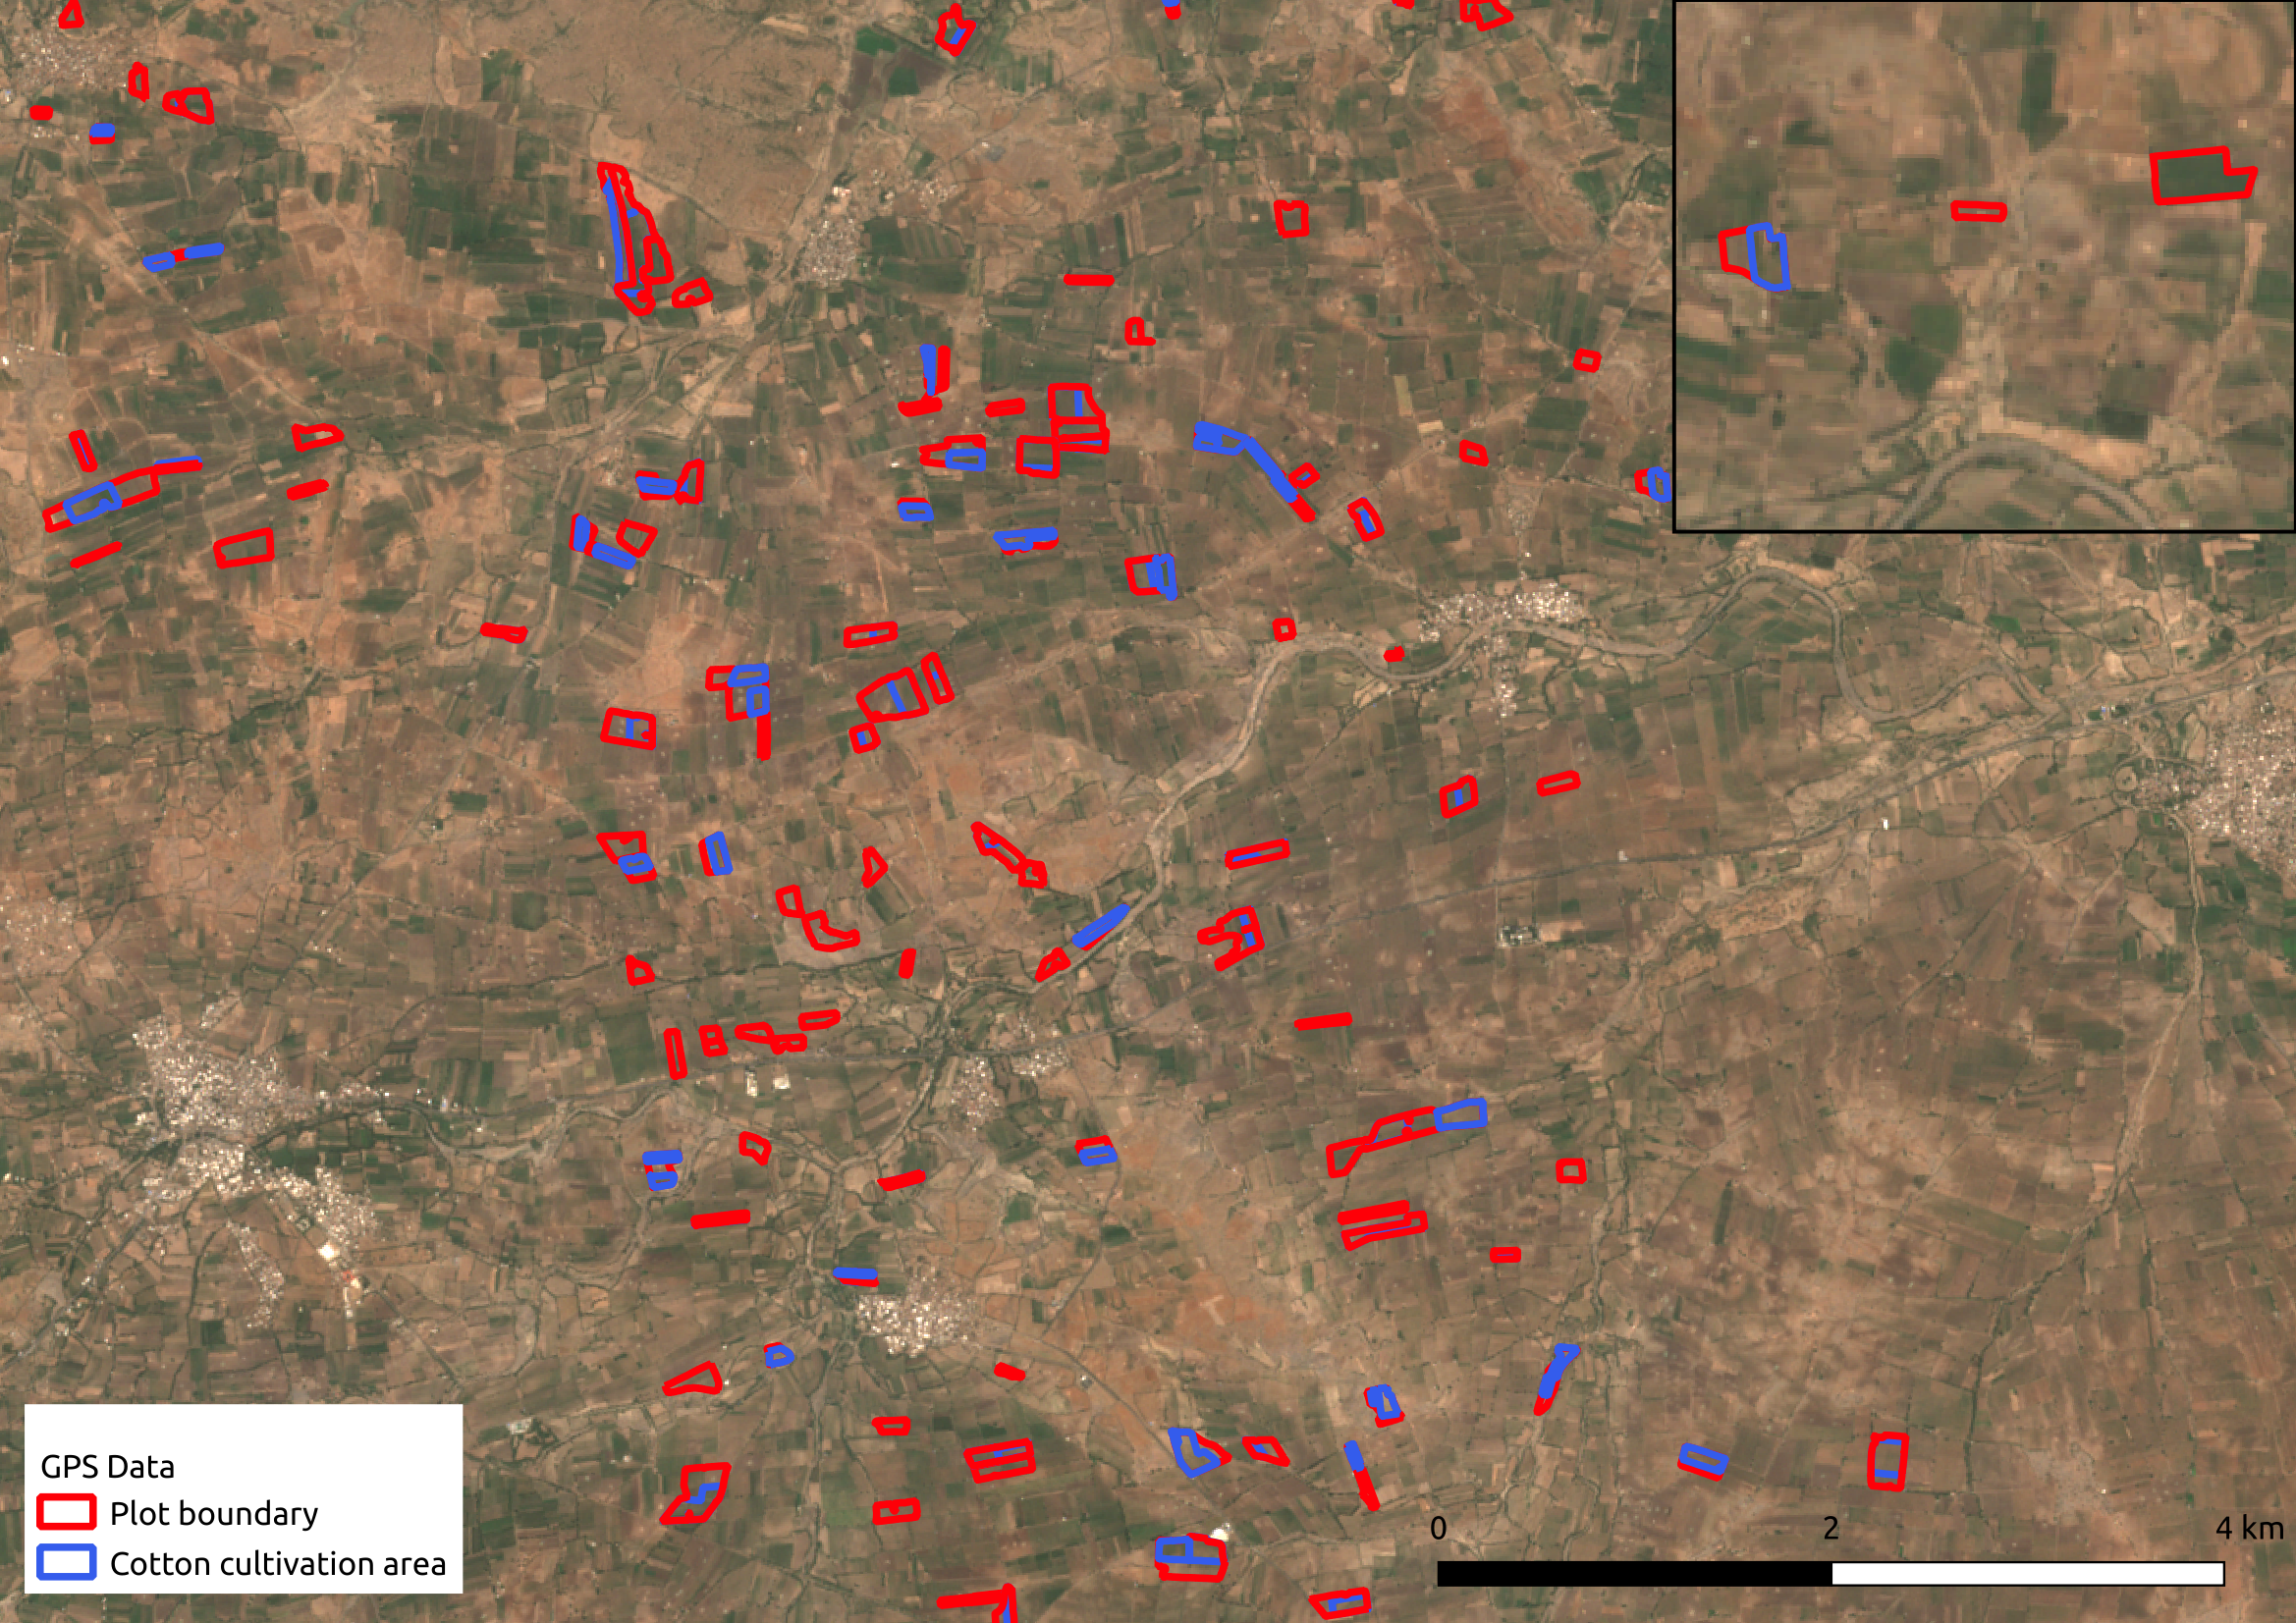
\includegraphics[width=6in]{figures/f1/true_color}} \\ \\
\subcaptionbox{reNDVI}{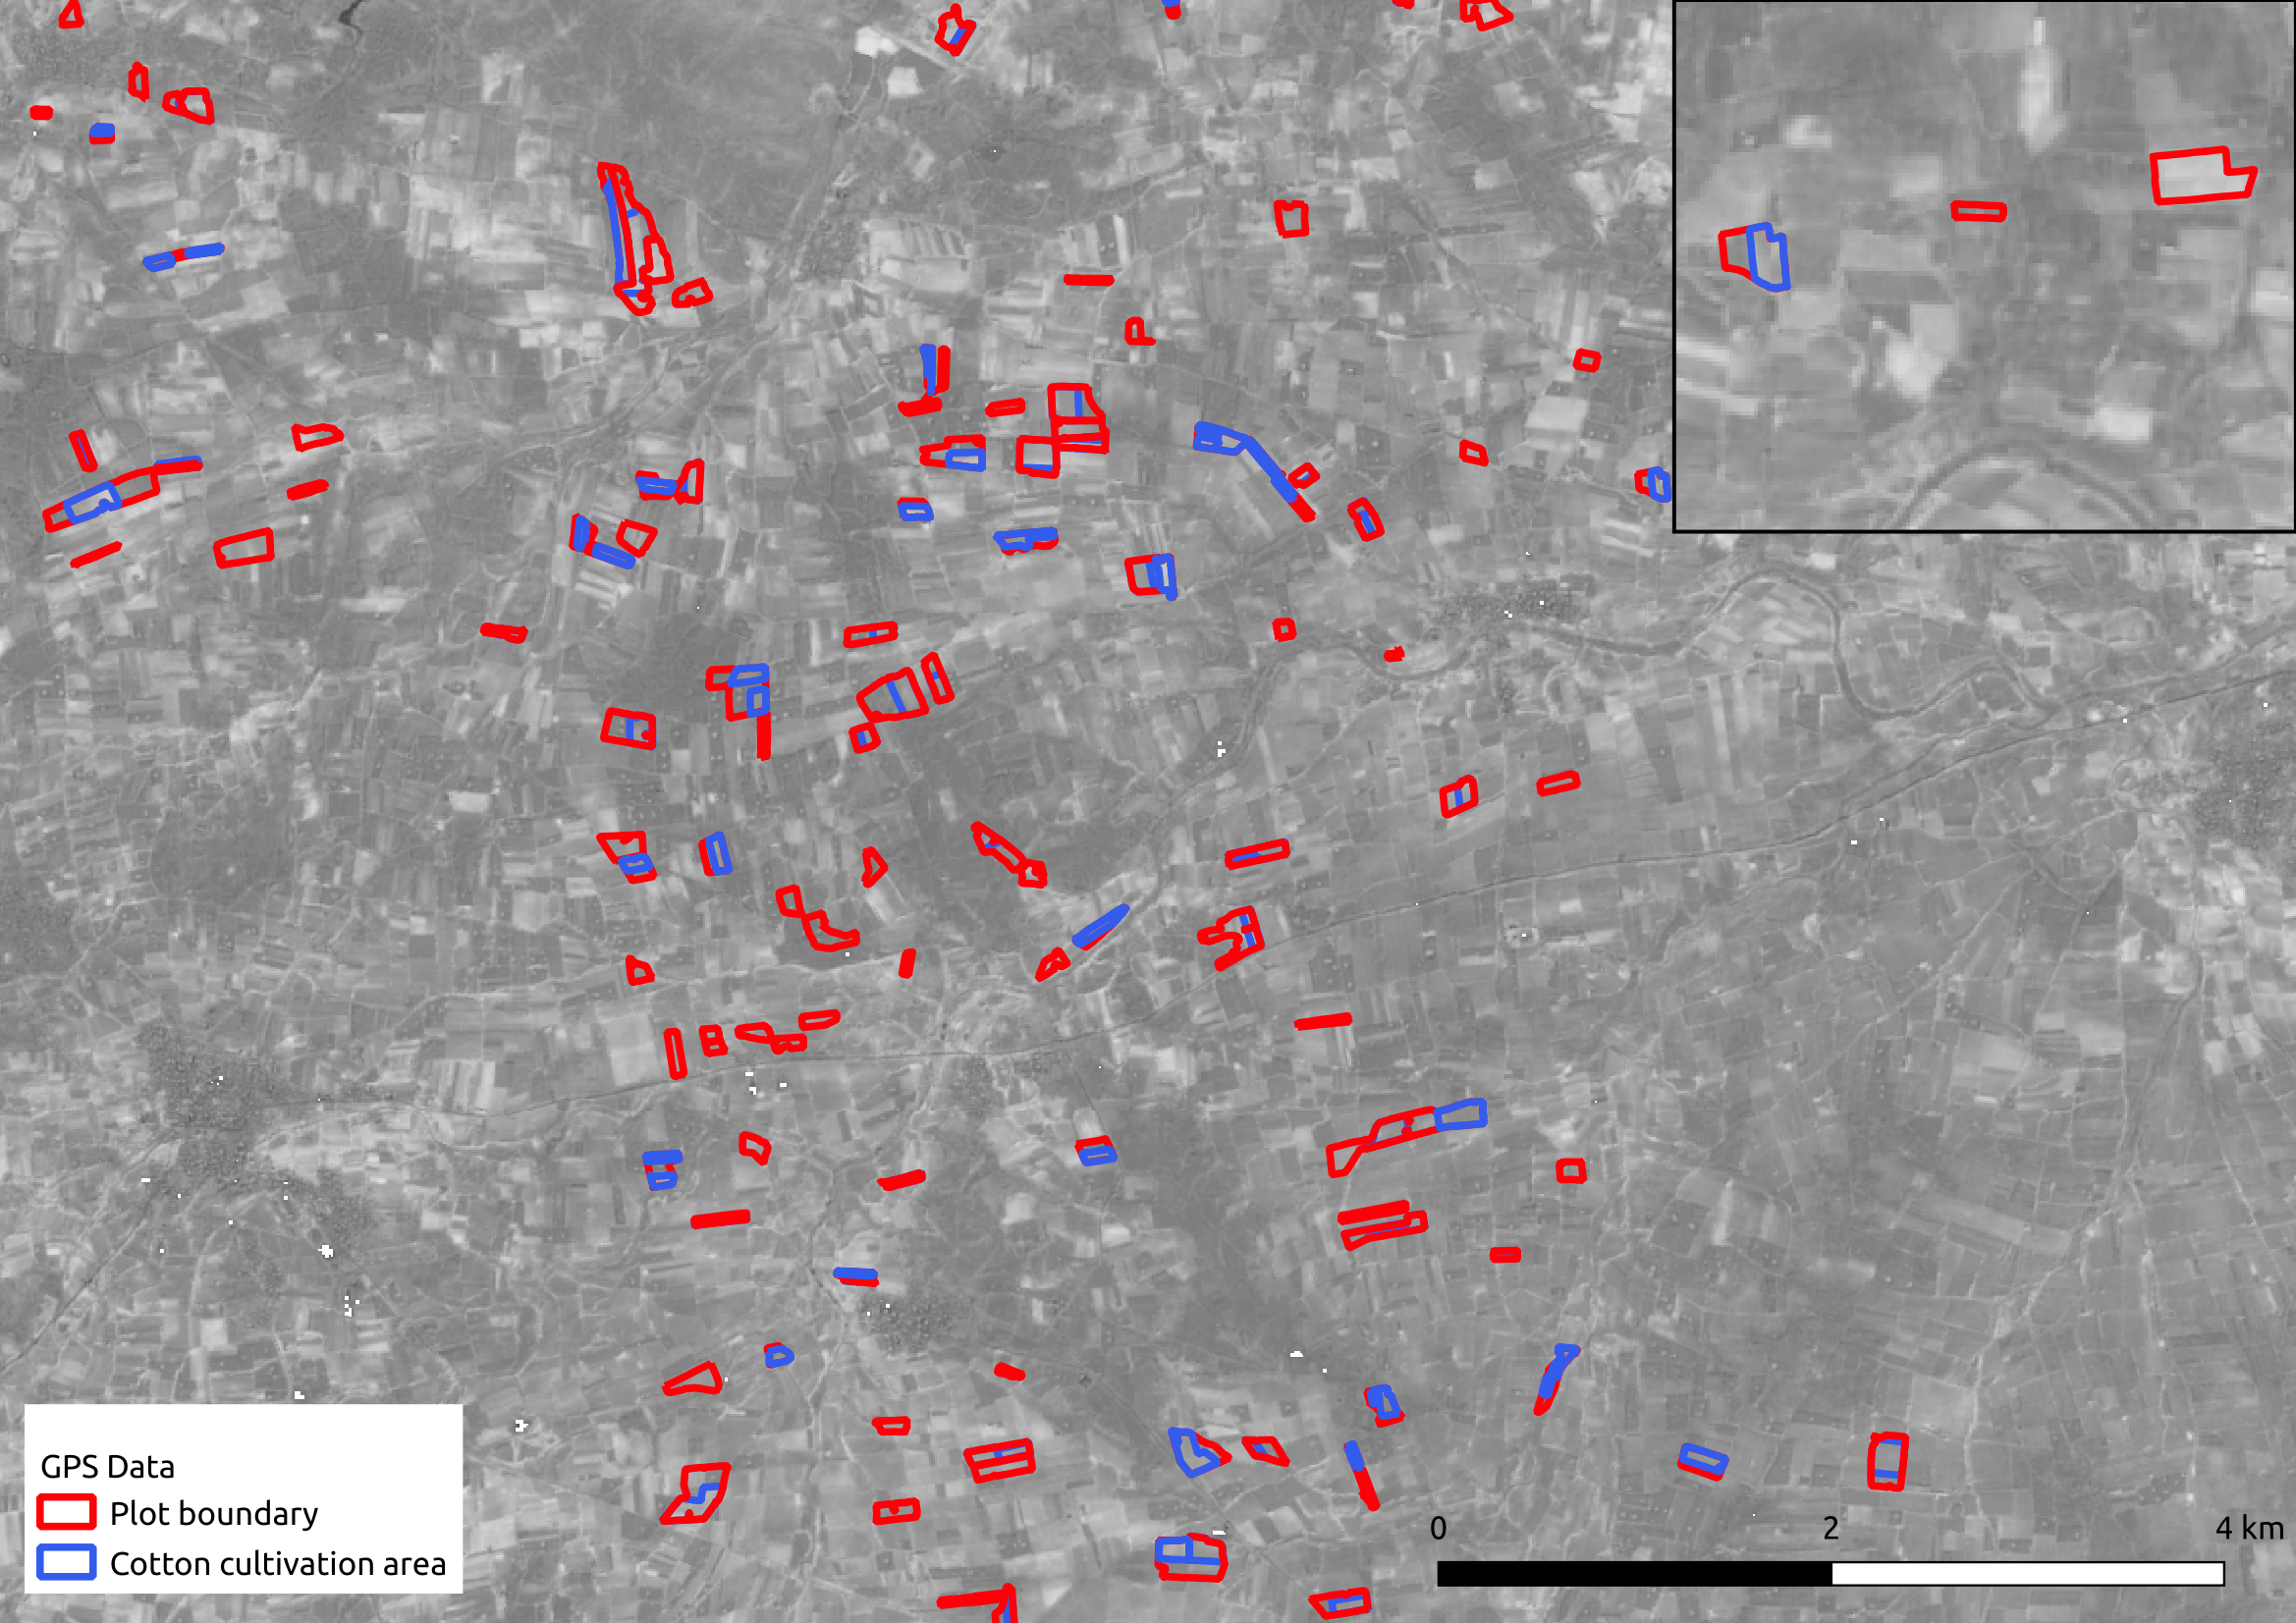
\includegraphics[width=6in]{figures/f1/ndvi}} \\
\multicolumn{1}{@{}m{0.95\textwidth}@{}}{\footnotesize Figure \ref{f:sentinel-imagery} presents sample Sentinel-2 imagery collected on October 28th, 2018 in a portion of the sample region that was selected due to a high density of sample plots. Panel (a) presents a true color composite. Panel (b) presents a reNDVI image, which is the vegetation index used for satellite productivity measurements in this paper. Polygons in red represent the boundaries of sample plots. Polygons in blue show the area on which the farmer cultivated cotton, if they did not cultivate cotton on their full plot.}
\end{tabular}
\end{figure}

\FloatBarrier

\pagebreak
\clearpage

\begin{figure}[!htb] \centering \caption{Applied minus recommended fertilizer, basal dose (kg/ha)} \label{f:fertilizer-gap-basal}
\begin{tabular}{cc}
\subcaptionbox{UREA}{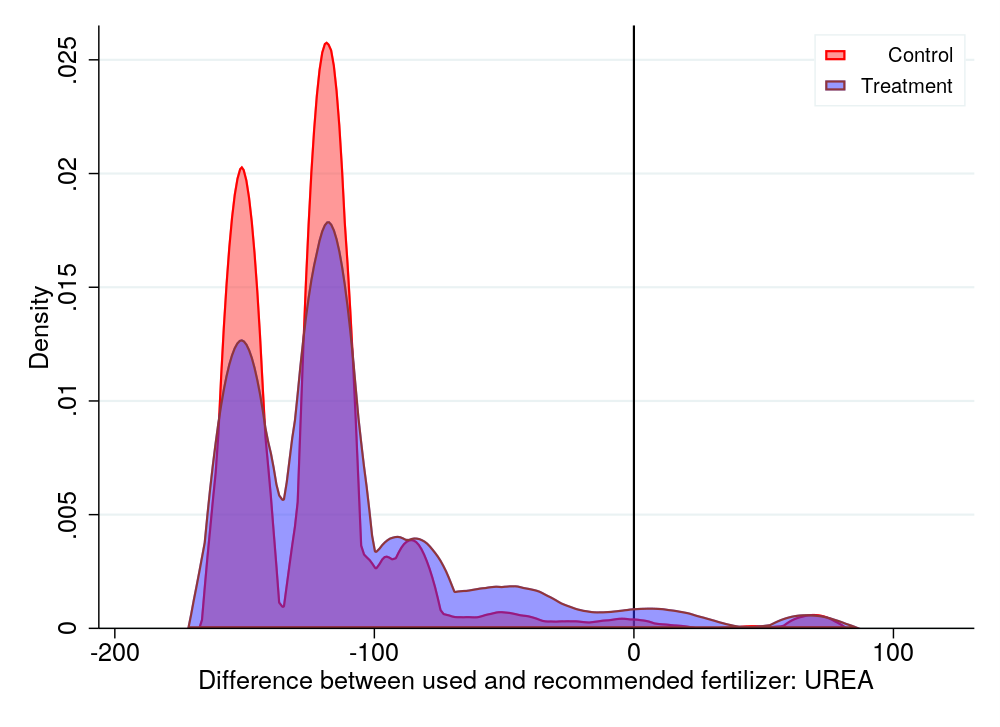
\includegraphics[width=3.5in]{figures/f2/UREA}} & 
\subcaptionbox{DAP}{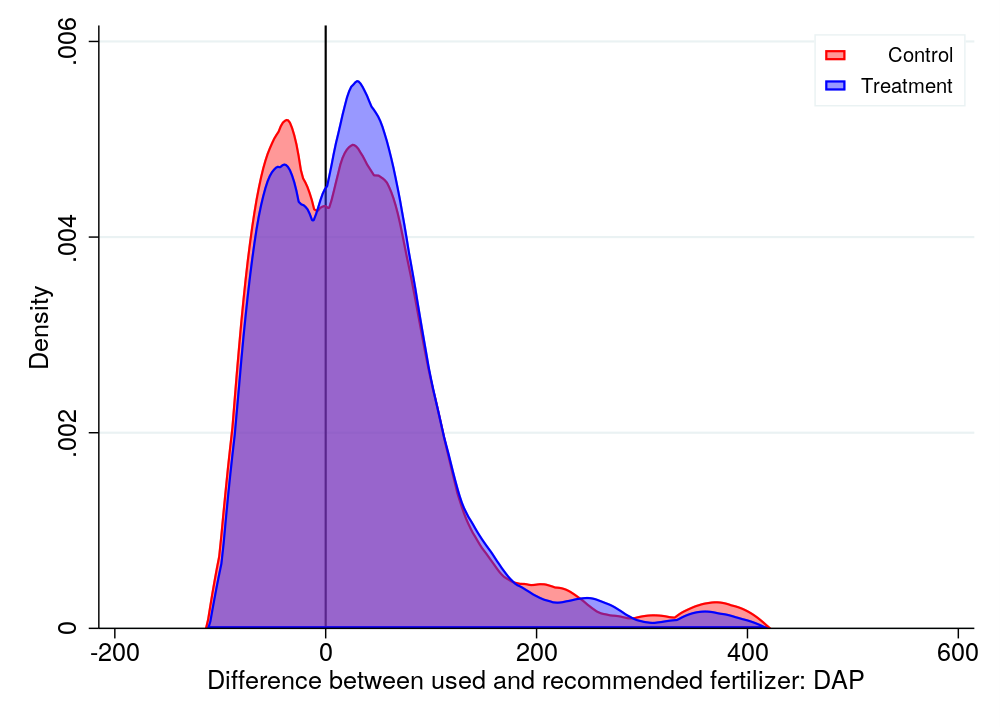
\includegraphics[width=3.5in]{figures/f2/DAP}} \\
\subcaptionbox{MOP}{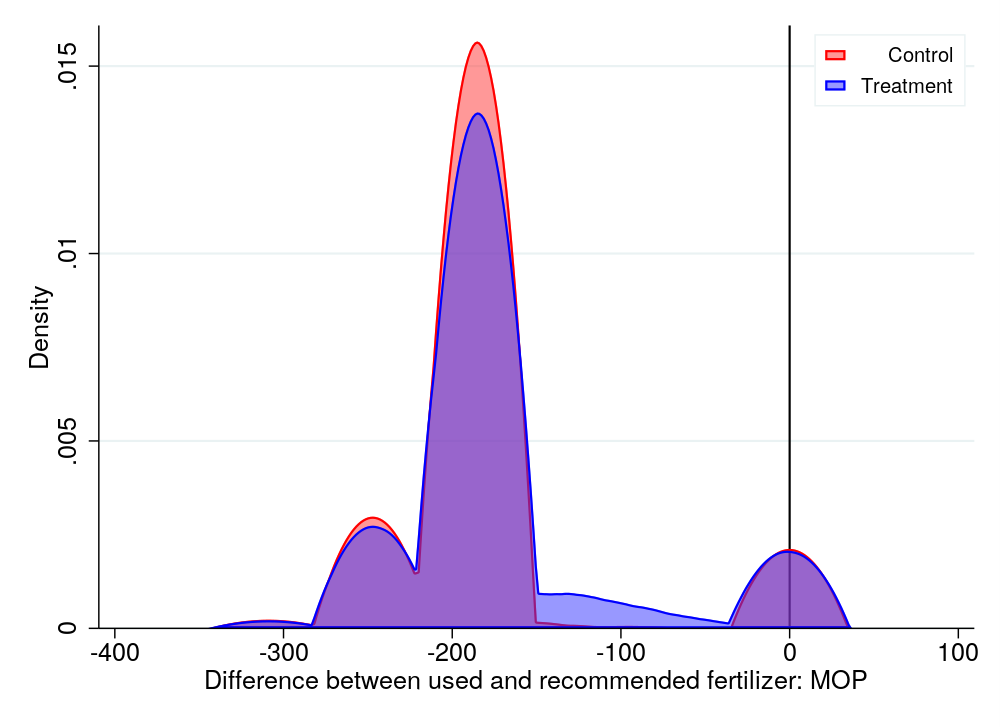
\includegraphics[width=3.5in]{figures/f2/MOP}} & 
\subcaptionbox{Zinc}{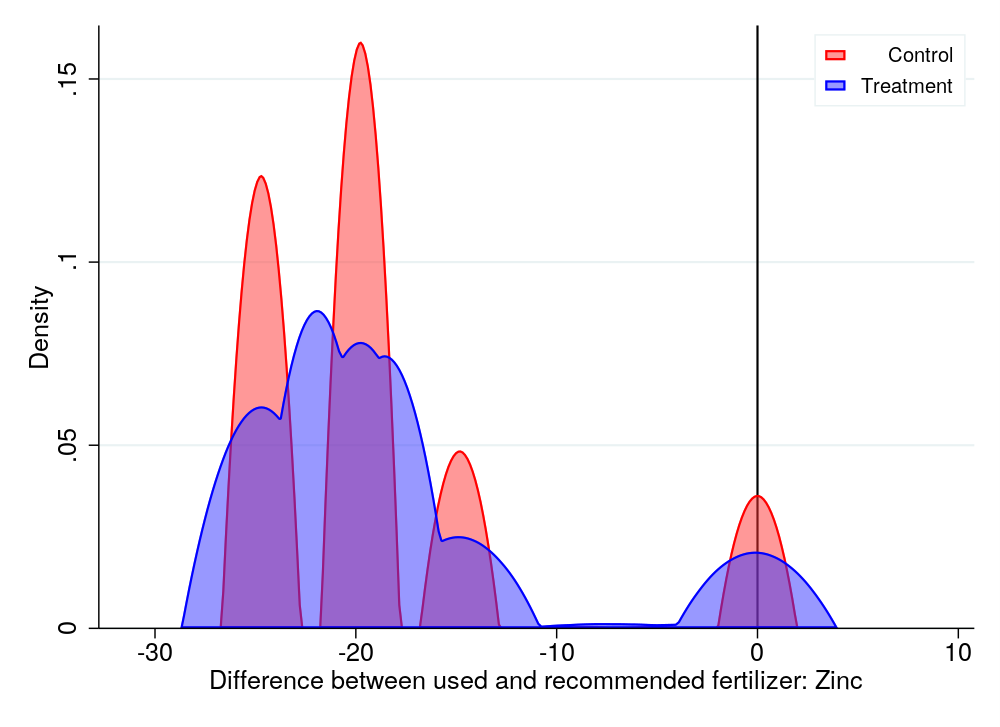
\includegraphics[width=3.5in]{figures/f2/ZINC}} \\
\multicolumn{2}{@{}m{0.95\textwidth}@{}}{\footnotesize Figure \ref{f:fertilizer-gap-basal} displays kernel density estimates for the difference between the applied and recommended basal fertilizer dose in kg/ha. Differences were calculated by subtracting the lab recommended fertilizer dose from the farmer's self-reported use. The density plots use a Epanechnikov kernel function. Estimates were calculated separately for treatment (red) and control (blue). Values below 0 indicate that the farmer applied less than the recommended dose, and values above 0 indicate that the farmer applied more than the recommended dose. Differences are winsorized at the 99th percentile.}
\end{tabular}
\end{figure}

\FloatBarrier

\pagebreak
\clearpage

\begin{figure}[!htb] \centering \caption{Applied minus recommended fertilizer, total (kg/ha)} \label{f:fertilizer-gap-total}
\begin{tabular}{cc}
\subcaptionbox{UREA}{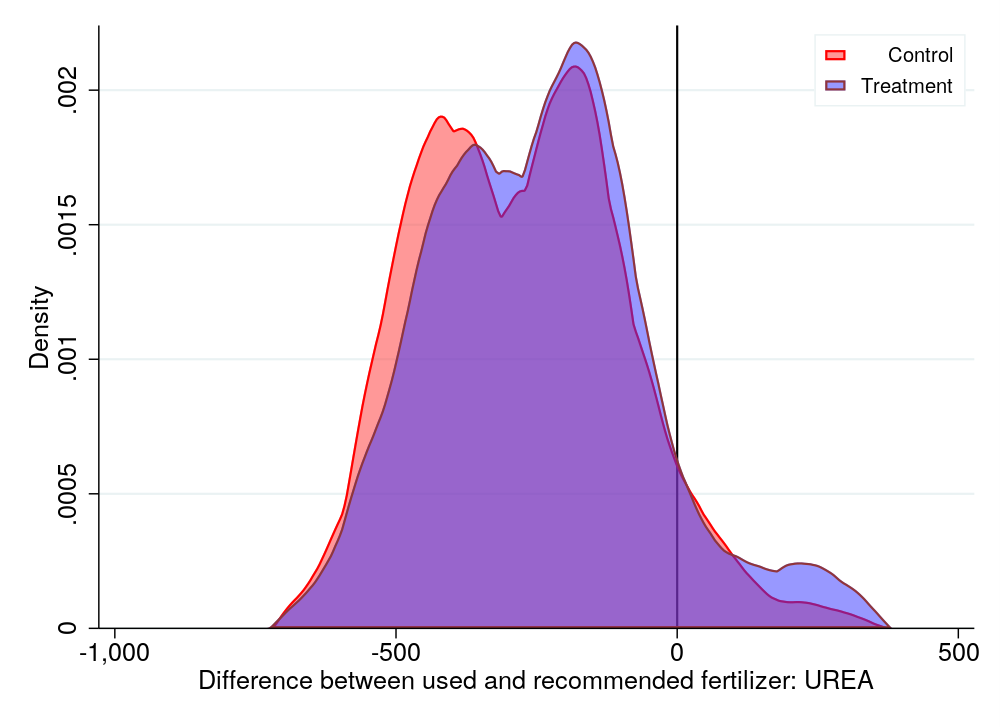
\includegraphics[width=3.5in]{figures/f3/urea}} & 
\subcaptionbox{DAP}{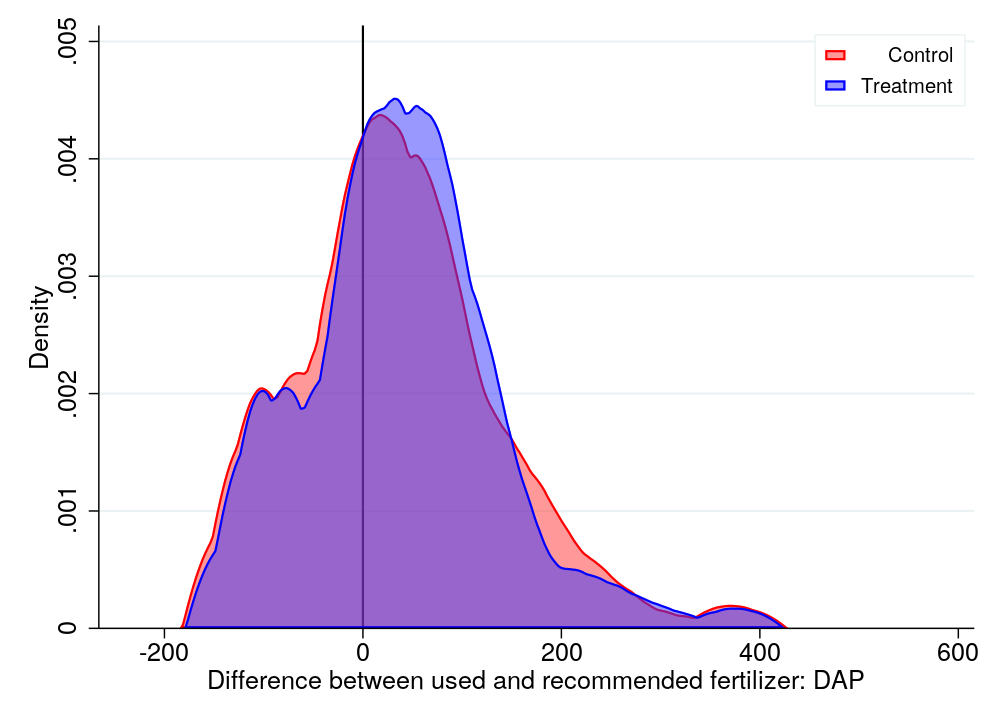
\includegraphics[width=3.5in]{figures/f3/dap}} \\
\subcaptionbox{MOP}{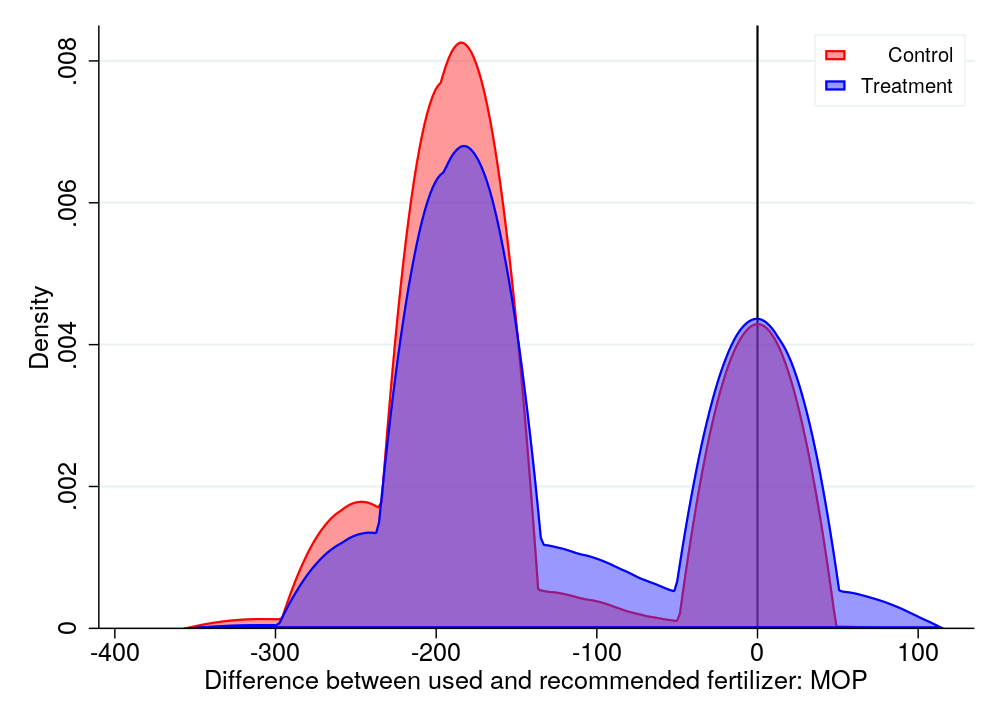
\includegraphics[width=3.5in]{figures/f3/mop}} & 
\subcaptionbox{Zinc}{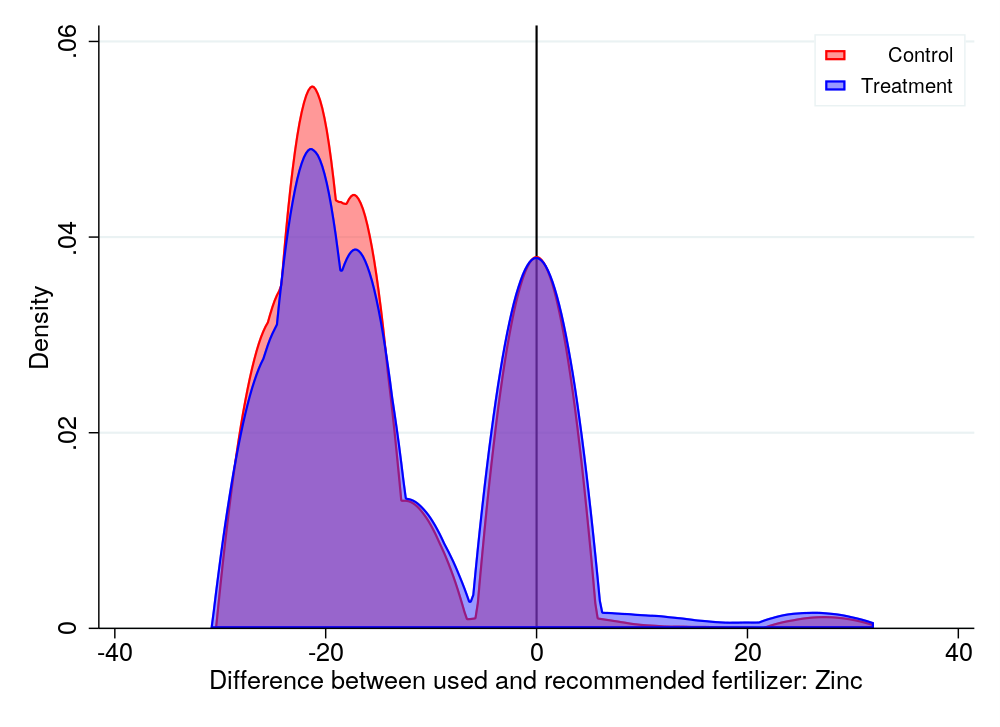
\includegraphics[width=3.5in]{figures/f3/zinc}} \\
\multicolumn{2}{@{}m{0.95\textwidth}@{}}{\footnotesize Figure \ref{f:fertilizer-gap-total} displays kernel density estimates for the difference between the applied and recommended total fertilizer application (across the full growing season) in kg/ha. Differences were calculated by subtracting the lab recommended fertilizer dose from the farmer's self-reported use. The density plots use a Epanechnikov kernel function. Estimates were calculated separately for treatment (red) and control (blue). Values below 0 indicate that the farmer applied less than the recommended amount, and values above 0 indicate that the farmer applied more than the recommended amount. Differences are winsorized at the 99th percentile.}
\end{tabular}
\end{figure}

\FloatBarrier

\pagebreak
\clearpage

\begin{figure}[!htb] \centering \caption{Cotton yields (kg/ha)} \label{f:yields}
\begin{tabular}{cc}
\subcaptionbox{Survey data}{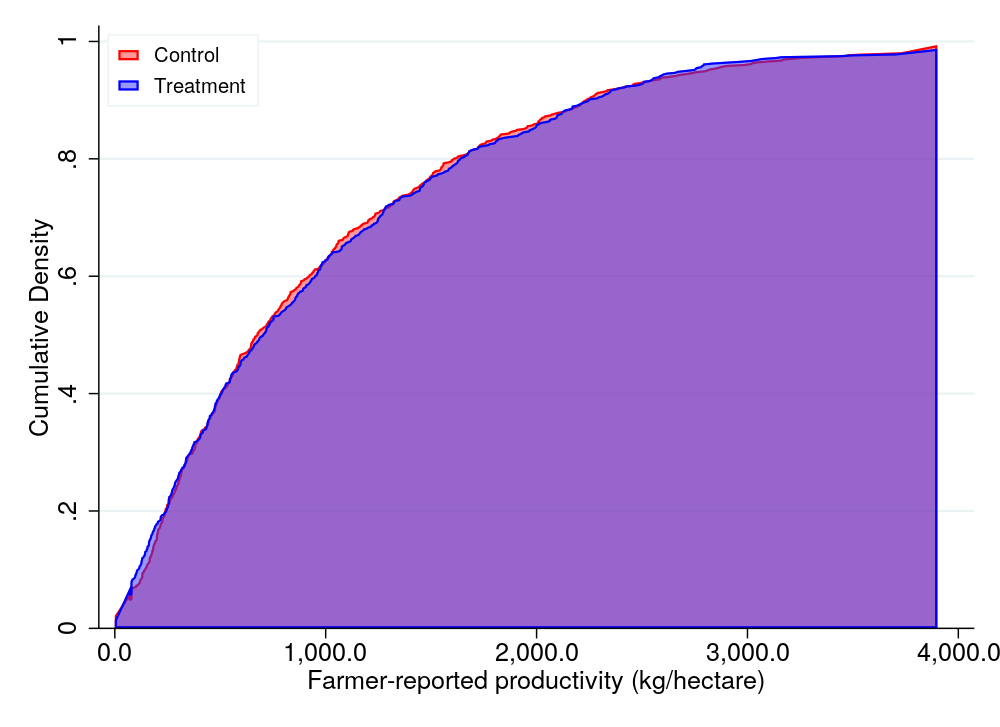
\includegraphics[width=3.5in]{figures/f4/yields_survey.png}} & 
\subcaptionbox{Satellite data}{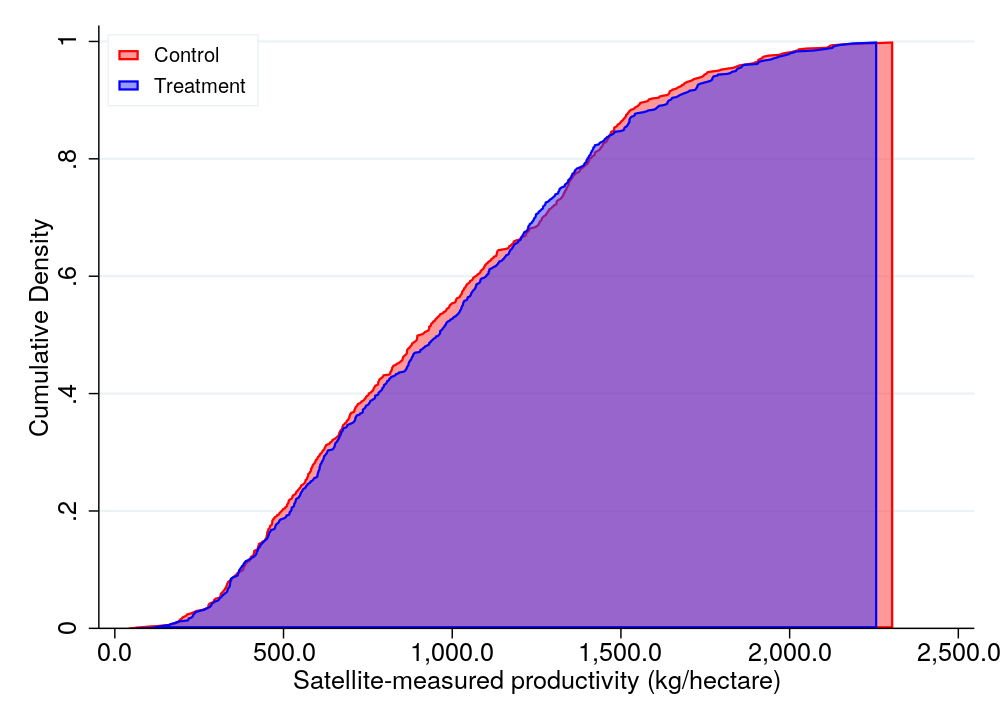
\includegraphics[width=3.5in]{figures/f4/yields_satellite.png}} \\
\multicolumn{2}{@{}m{0.95\textwidth}@{}}{\footnotesize Figure \ref{f:yields} displays cumulative density plots of productivity in kg/ha. Panel (a) uses farmer-reported total yields divided by the GPS-measured area on which the farmer grew cotton. Positive yield values are winsorized at the 2nd and 98th percentiles. Panel (b) displays satellite measured yields based on a reNDVI \citep{Vina2005NewCrops} calculated from Sentinel-2 L2A imagery. We constructed satellite yield measurements by calculating the median value of reNDVI values contained within each plot in the sample on 5 dates and then taking the maximum reNDVI across the 5 images for each plot. We then this value was linearly fitted to farmer-reported yield data. Several linear predictions were negative and were recoded to 0.}
\end{tabular}
\end{figure}

\FloatBarrier

\pagebreak
\clearpage

\begin{figure}[!htb] \centering \caption{Rainfall} \label{f:rainfall}
\begin{tabular}{c}
\subcaptionbox{Monthly}{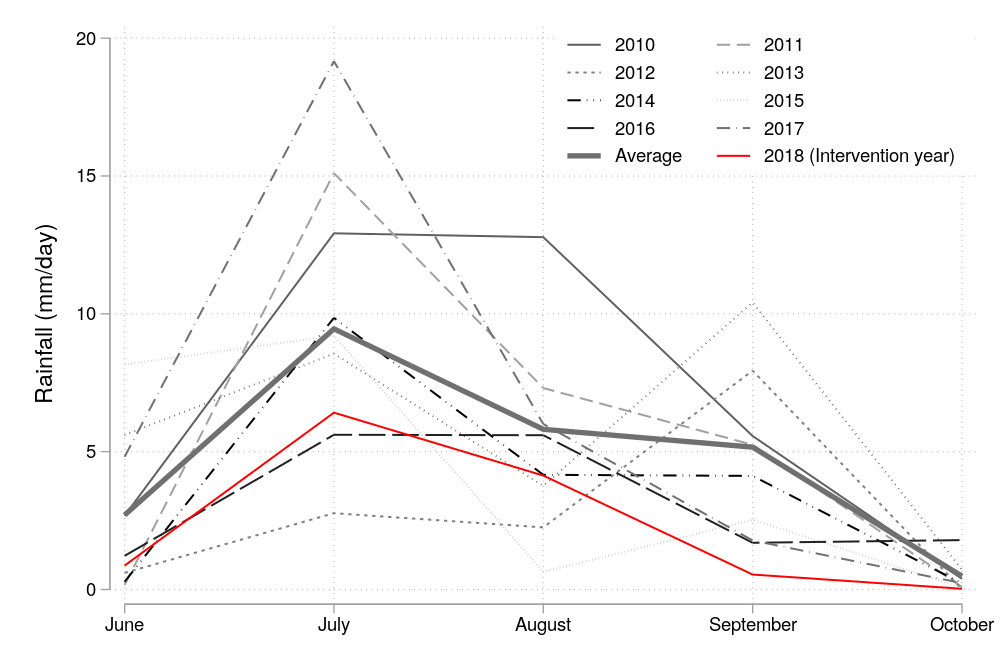
\includegraphics[width=6in]{figures/f5/rain_monthly.png}} \\ 
\subcaptionbox{Daily}{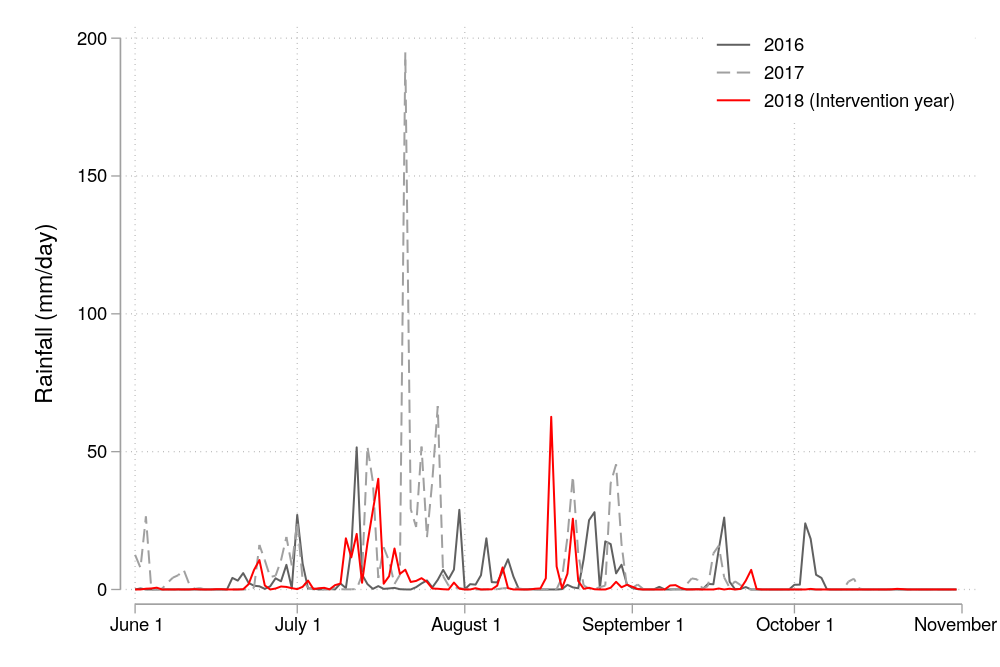
\includegraphics[width=6in]{figures/f5/rain_daily.png}} \\
\multicolumn{1}{@{}m{0.95\textwidth}@{}}{\footnotesize Figure \ref{f:rainfall} plots average rainfall across the sample. Rainfall data was obtained from NASA's Global Participation Measurement mission. The figures use final run IMERG data accessed through the Google Earth Engine. Sub-plot (a) presents monthly rainfall values, in mm/day, from 2010-2019. The average value from 2010-2019 is also reported. Sub-plot (b) displays daily rainfall data from 2016-2019.}
\end{tabular}
\end{figure}

\FloatBarrier

\pagebreak
\clearpage

\begin{figure}[!htb] \centering \caption{Sentinel-2 vegetation indices vs farmer-reported yield (kg/ha)} \label{f:fr-vs-satellite-yields}
\begin{tabular}{cc}
\subcaptionbox{NDVI}{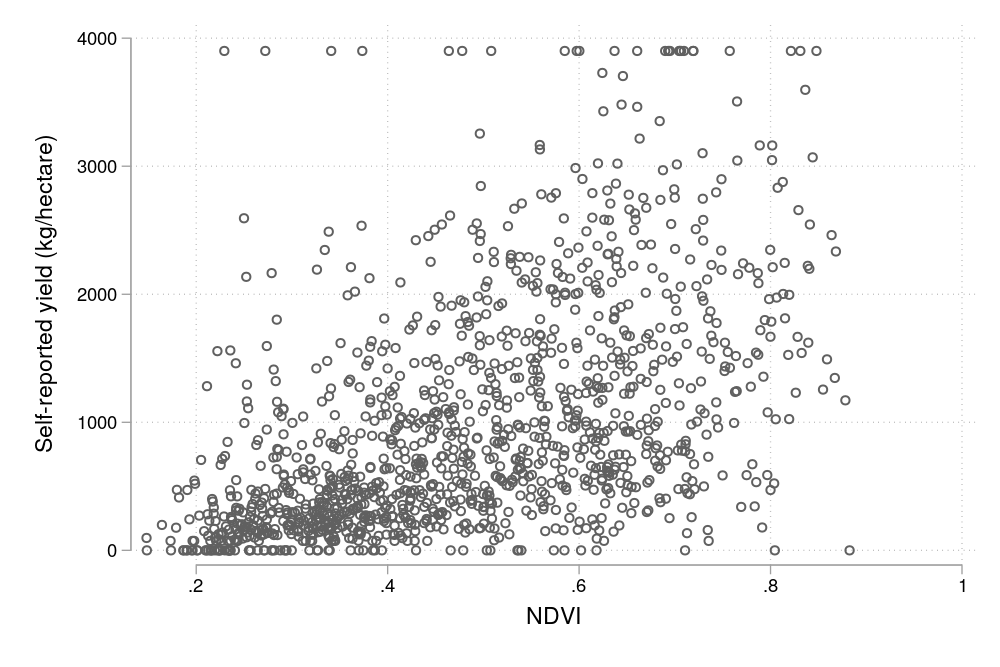
\includegraphics[width=3.5in]{figures/f6/NDVI}} & 
\subcaptionbox{GCVI}{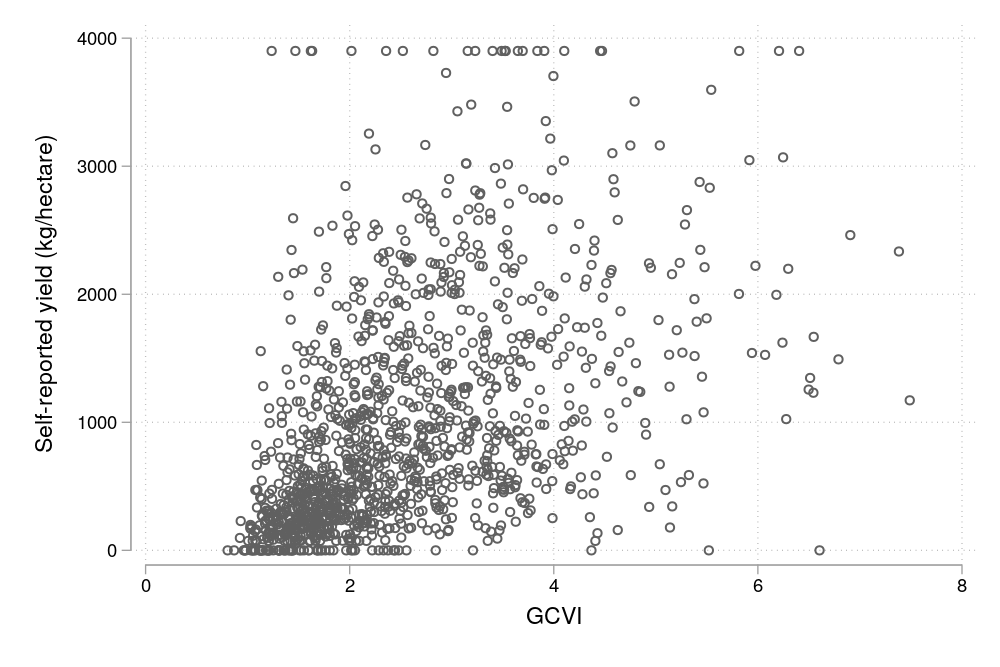
\includegraphics[width=3.5in]{figures/f6/GCVI}} \\
\subcaptionbox{reNDVI}{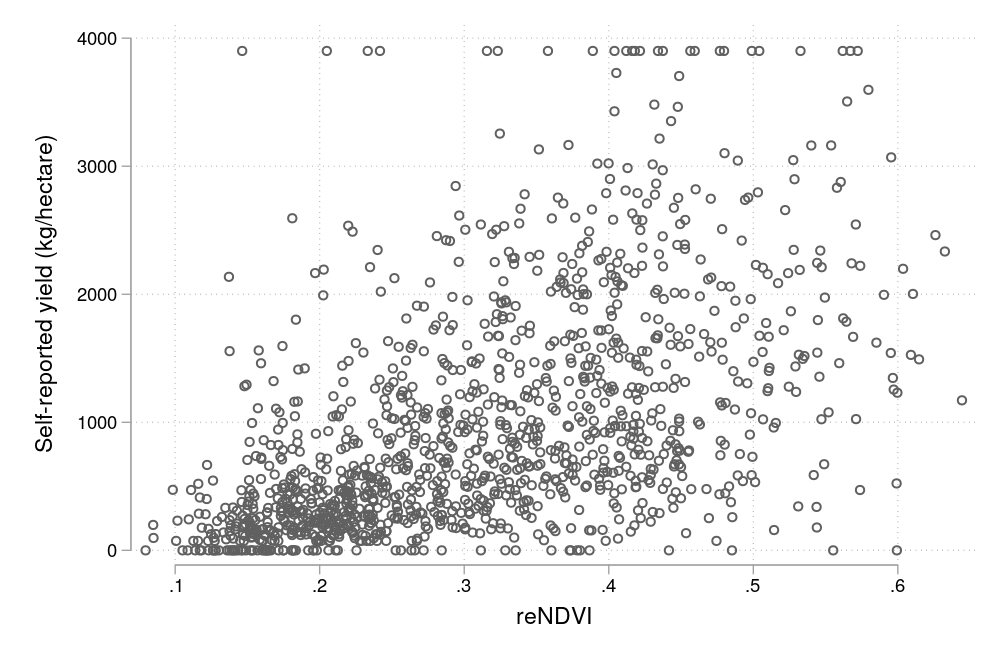
\includegraphics[width=3.5in]{figures/f6/reNDVI}} & 
\subcaptionbox{MTCI}{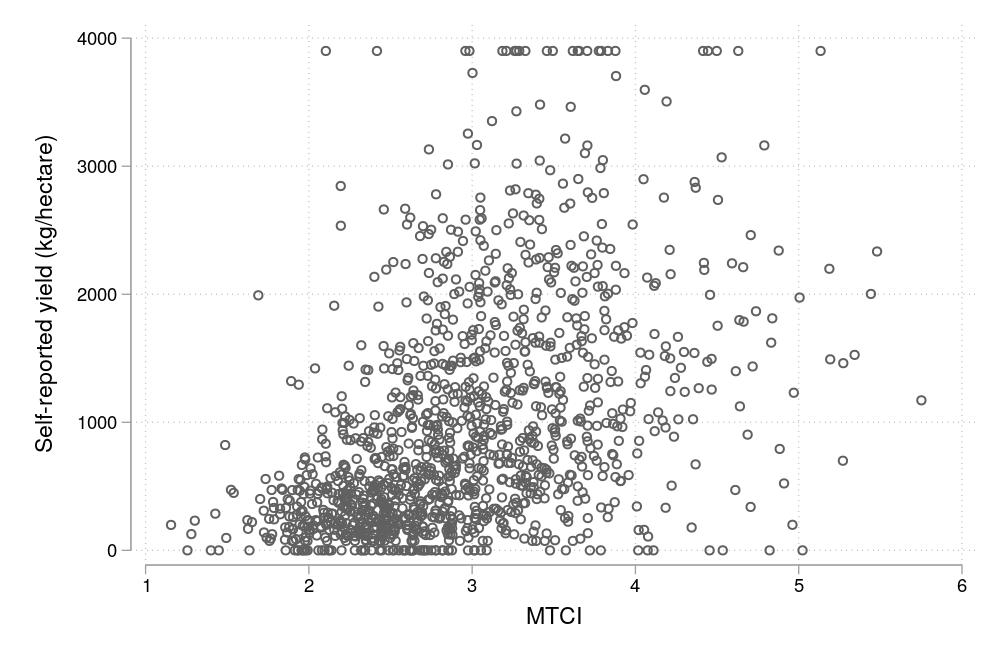
\includegraphics[width=3.5in]{figures/f6/MTCI}} \\
\multicolumn{2}{c}{\subcaptionbox{LAI}{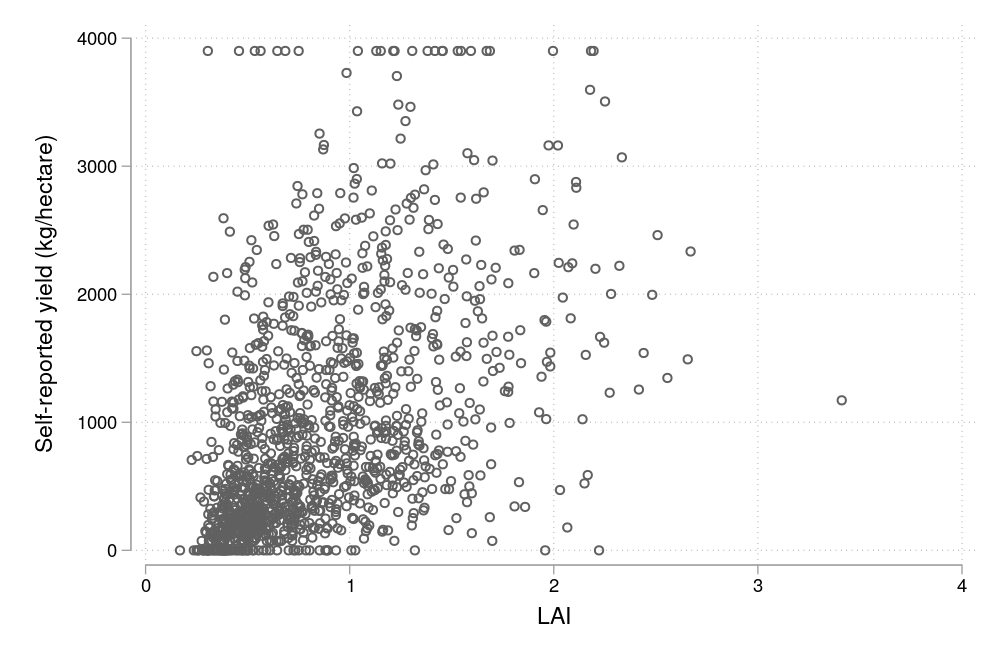
\includegraphics[width=3.5in]{figures/f6/LAI}}} \\
\multicolumn{2}{@{}m{0.95\textwidth}@{}}{\footnotesize Figure \ref{f:fr-vs-satellite-yields} plots vegetation index (VI) values against farmer-reported productivity. We calculated VI values by taking the median value of each VI pixel contained in each sample plot for 5 Sentinel-2 images from 2018. We then took the maximum value across the 5 satellite images. Farmer-reported yield was calculated by taking farmer-reported total harvest data and dividing it by GPS-measured plot area. Positive farmer-reported yield values were winsorized at the 2nd and 98th percentiles.}
\end{tabular}
\end{figure}

\FloatBarrier

\pagebreak
\clearpage

\begin{figure}[!htb] \centering \caption{Treatment effect confidence intervals \\ Farmer-reported vs satellite measurements} \label{f:confidence_intervals}
\begin{tabular}{c}
\subcaptionbox{Monthly}{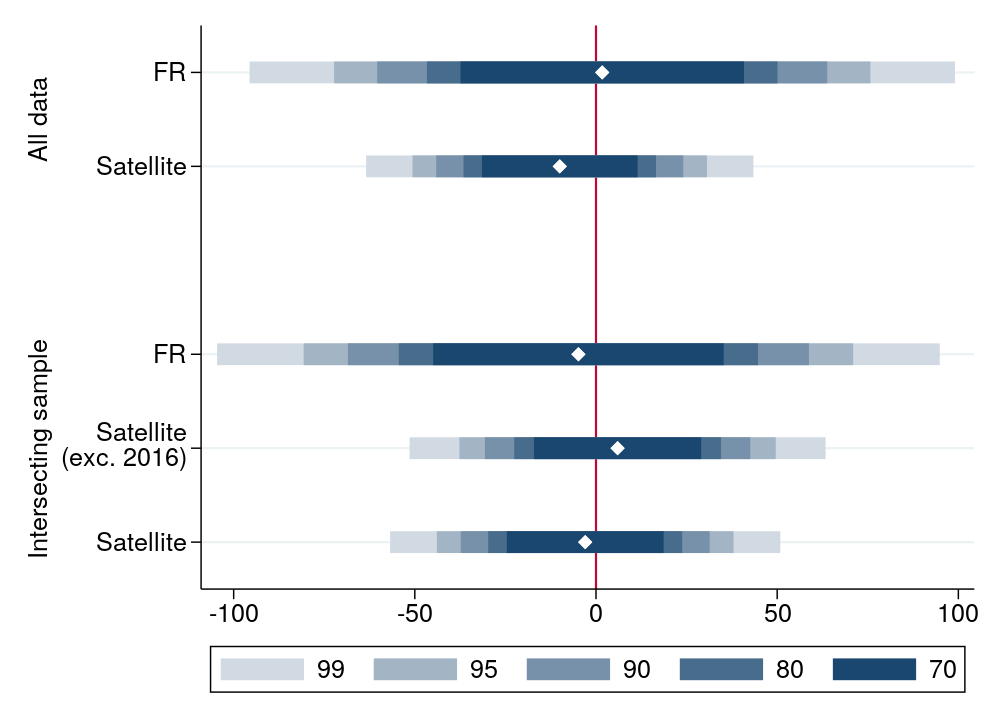
\includegraphics[width=0.95\linewidth]{figures/f7/confidence_intervals}} \\ 
\multicolumn{1}{@{}m{0.95\textwidth}@{}}{\footnotesize Figure \ref{f:confidence_intervals} plots confidence intervals of the treatment effect on productivity using farmer-reported and satellite yield data. The first two rows use all available data, and the bottom three rows examine a restricted sample of data that is not missing for either data source. Rows 1 and 3 examine farmer-reported yield data, and each of the other rows use satellite measurements. Rows 1, 2, and 4 control for 2017 productivity. Rows 3 and 5 control for 2016 and 2017 productivity. All regressions include block fixed effects and robust standard errors.}
\end{tabular}
\end{figure}

\pagebreak

\clearpage

\begin{center}
\section*{Tables}
\end{center}
\clearpage

\FloatBarrier

\begin{table}[!htp] \centering
\def\sym#1{\ifmmode^{#1}\else\(^{#1}\)\fi}
\caption{Summary statistics, baseline} \label{t:balance}
\begin{tabularx}{\linewidth}{@{}Xccccccc@{}}
\hline \hline \\[-2mm]
&\multicolumn{1}{c}{(1)}&\multicolumn{1}{c}{(2)}&\multicolumn{1}{c}{(3)}&\multicolumn{1}{c}{(4)}&\multicolumn{1}{c}{(5)}&\multicolumn{1}{c}{(6)}&\multicolumn{1}{c}{(7)}\\
&\multicolumn{1}{c}{\makecell[c]{Control \\ (full sample)}}&\multicolumn{1}{c}{\makecell[c]{Treatment - Control \\ (full sample)}}&\multicolumn{1}{c}{\makecell[c]{T-C \\ (basal)}}&\multicolumn{1}{c}{\makecell[c]{T-C \\ (midline)}}&\multicolumn{1}{c}{\makecell[c]{T-C \\ (endline)}}&\multicolumn{1}{c}{\makecell[c]{T-C \\ (farmer-reported \\ yield)}}&\multicolumn{1}{c}{\makecell[c]{T-C \\ (satellite \\ data)}}\\
\hline
\\[-2mm]
Age (baseline) &    42.600 & -0.155 & -0.464 & 0.036 & -0.073 & 0.020 & -0.153 \\ 
 & [11.485] & (0.604) & (0.633) & (0.611) & (0.623) & (0.637) & (0.643) \\ [1em] 
Literate &     0.845 & -0.017 & -0.016 & -0.023 & -0.024 & -0.028 & -0.024 \\ 
 & [0.362] & (0.019) & (0.020) & (0.019) & (0.020) & (0.020) & (0.020) \\ [1em] 
Total cotton land (2017) &     3.602 & -0.189 & -0.124 & -0.180 & -0.197 & -0.236 & -0.090 \\ 
 & [3.735] & (0.187) & (0.201) & (0.189) & (0.191) & (0.196) & (0.184) \\ [1em] 
Sampled plot size (2017) &     2.080 & -0.075 & -0.040 & -0.089 & -0.103 & -0.111 & -0.073 \\ 
 & [1.677] & (0.082) & (0.087) & (0.081) & (0.083) & (0.085) & (0.085) \\ [1em] 
Irrigation &     0.911 & -0.024 & -0.016 & -0.030\sym{*} & -0.022 & -0.031\sym{*} & -0.016 \\ 
 & [0.285] & (0.015) & (0.016) & (0.016) & (0.016) & (0.016) & (0.016) \\ [1em] 
Strong house &     0.613 & 0.018 & 0.025 & 0.020 & 0.010 & 0.004 & 0.003 \\ 
 & [0.487] & (0.025) & (0.026) & (0.025) & (0.026) & (0.026) & (0.027) \\ [1em] 
Own plough &     0.420 & 0.009 & -0.008 & 0.012 & 0.007 & 0.001 & 0.016 \\ 
 & [0.494] & (0.025) & (0.027) & (0.026) & (0.026) & (0.027) & (0.027) \\ [1em] 
Crop insurance &     0.570 & -0.008 & -0.007 & -0.005 & -0.009 & -0.009 & -0.021 \\ 
 & [0.495] & (0.025) & (0.027) & (0.026) & (0.026) & (0.027) & (0.027) \\ [1em] 
Children &     2.415 & -0.101 & -0.133\sym{*} & -0.090 & -0.104 & -0.093 & -0.107 \\ 
 & [1.346] & (0.068) & (0.070) & (0.069) & (0.071) & (0.073) & (0.073) \\ [1em] 
$>$ median education &     0.377 & -0.015 & -0.006 & -0.019 & -0.018 & -0.017 & -0.019 \\ 
 & [0.485] & (0.025) & (0.026) & (0.025) & (0.026) & (0.026) & (0.026) \\ [1em] 
Soil tested prior to study &     0.142 & -0.016 & -0.016 & -0.013 & -0.017 & -0.021 & -0.012 \\ 
 & [0.349] & (0.018) & (0.019) & (0.018) & (0.018) & (0.019) & (0.019) \\ [1em] 
UREA last season (kg/ha) &   292.328 & -19.055 & -5.956 & -20.435 & -23.589 & -27.914 & -23.270 \\ 
 & [444.784] & (17.328) & (9.115) & (17.794) & (18.552) & (19.225) & (19.568) \\ [1em] 
DAP last season (kg/ha) &   156.450 & -7.555 & -8.901 & -8.490 & -8.777 & -10.367 & -8.882 \\ 
 & [207.443] & (9.747) & (10.601) & (10.009) & (10.418) & (10.852) & (10.977) \\ [1em] 
MOP last season (kg/ha) &     5.293 & 0.332 & 0.292 & 0.020 & -0.024 & -0.100 & 0.109 \\ 
 & [23.010] & (1.215) & (1.303) & (1.226) & (1.278) & (1.309) & (1.342) \\ [1em] 
Zinc last season (kg/ha) &     1.264 & 0.985 & 1.001 & 0.956 & 0.505 & 0.444 & 0.648 \\ 
 & [6.557] & (0.632) & (0.696) & (0.647) & (0.400) & (0.413) & (0.418) \\ [1em] 
Observations & 755 &     1,516 &     1,375 &     1,469 &     1,402 &     1,341 &     1,323 \\ 
p-value of joint orthogonality &  &     0.530 &     0.696 &     0.418 &     0.566 &     0.436 &     0.643 \\ 

\hline
\multicolumn{8}{@{}m{\linewidth}@{}}{\footnotesize Standard deviations in brackets. Standard errors in parenthesis. \sym{*} \(p<0.10\), \sym{**} \(p<0.05\), \sym{***} \(p<0.01\)} \\
\multicolumn{8}{@{}m{\linewidth}@{}}{\footnotesize Column (1) reports the control group mean of the indicated variable across all baseline respondents. Column (2) reports the difference in means between the control and treatment groups across the full sample of baseline respondents. Columns (3), (4), and (5), report the same value, but among respondents that completed the basal survey, midline survey, and endline survey. Column (6) restricts the sample to observations for which farmer-reported yields are non-missing. Column (7) restricts the sample to observations for which satellite yield measurements are available for 2016, 2017, and 2018. Education data was missing for 175 observations. Number of children is missing for 25 observations. Crop insurance is missing for 20 observations. UREA and DAP usage last season are missing for 3 observations, DAP and MOP usage last season are missing for two observations, and sampled plot size is missing for one observations. We interpolated the missing values of these variables using the median value of each variable.}
\end{tabularx}
\end{table}
\FloatBarrier

\pagebreak
\clearpage

\begin{table}[!ht] \centering \caption{Treatment effect on KT Call Engagement, and Knowledge} \label{t:engagement-and-knowledge}
\def\sym#1{\ifmmode^{#1}\else\(^{#1}\)\fi}
\begin{tabularx}{\linewidth}{@{}XZZZZZZ@{}}
\hline \hline \\[-2mm]
 & \multicolumn{3}{c}{Administrative data} & \multicolumn{2}{c}{Endline survey} & \multicolumn{1}{c}{Midline survey} \\ \cmidrule(l{2pt}r{2pt}){2-4} \cmidrule(l{2pt}r{2pt}){5-6} \cmidrule(l{2pt}r{2pt}){7-7} 
&\multicolumn{1}{c}{(1)}&\multicolumn{1}{c}{(2)}&\multicolumn{1}{c}{(3)}&\multicolumn{1}{c}{(4)}&\multicolumn{1}{c}{(5)}&\multicolumn{1}{c}{(6)}\\
&\multicolumn{1}{c}{\makecell[c]{KT call \\ pickup \\ rate}}&\multicolumn{1}{c}{\makecell[c]{Share of \\ total content \\ heard}}&\multicolumn{1}{c}{\makecell[c]{KT call \\ rating}}&\multicolumn{1}{c}{\makecell[c]{Use mobile \\ phone advisory}}&\multicolumn{1}{c}{\makecell[c]{Trust in \\ mobile phone \\ advisory (1-5)}}&\multicolumn{1}{c}{\makecell[c]{Fertilizer \\ questions \\ correct}}\\
\hline
\\[-2mm]
\multicolumn{7}{l}{\textit{Panel A: Full sample}} \\ [1em]
\partialinput{4}{5}{tables/t2/kt_panel_a.tex} [1em]
\partialinput{9}{12}{tables/t2/kt_panel_a.tex}
\end{tabularx}
\begin{tabularx}{\linewidth}{@{}XZZZZZZ@{}}
\\[-2mm]
\multicolumn{7}{l}{\textit{Panel B: Respondents that provided yield data}} \\ [1em]
\partialinput{4}{5}{tables/t2/kt_panel_b.tex} [1em]
\partialinput{9}{12}{tables/t2/kt_panel_b.tex}
\end{tabularx}
\begin{tabularx}{\linewidth}{@{}XZZZZZZ@{}}
\\[-2mm]
\multicolumn{7}{l}{\textit{Panel C: Respondents for which satellite data is available}} \\ [1em]
\partialinput{4}{5}{tables/t2/kt_panel_c.tex} [1em]
\partialinput{9}{12}{tables/t2/kt_panel_c.tex}
\end{tabularx}
\begin{tabularx}{\linewidth}{@{}XZZZZZZ@{}}
\\[-2mm]
\multicolumn{7}{l}{\textit{Panel D: Respondents for which farmer-reported and satellite yields are available}} \\ [1em]
\partialinput{4}{5}{tables/t2/kt_panel_b.tex} [1em]
\partialinput{9}{12}{tables/t2/kt_panel_b.tex}
\hline
\multicolumn{7}{@{}m{\linewidth}@{}}{\footnotesize Robust standard errors in parenthesis. \sym{*} \(p<0.10\), \sym{**} \(p<0.05\), \sym{***} \(p<0.01\)} \\
\multicolumn{7}{@{}m{\linewidth}@{}}{\footnotesize The dependent variable in column (1) is the share of non-fertilizer KT calls that the farmer picked up. In column (2), the dependent variable is the average share of non-fertilizer KT calls that the farmer listened to. Column (3) is the ranking given by farmers to KT calls in terms of usefulness, where 1 means that the calls were not useful and 5 that the call were most useful. Column (4) examines whether farmers use a mobile phone advisory service to make agricultural decisions. In Column (5), the dependent variable records the respondent's reported trust in mobile phone-based advice on a scale of 1 (very low trust) to 5 (very high trust). Column (6) records the number of questions, out of 14, in a quiz aimed to assess fertilizer knowledge were answered correctly. The sample size is lower in column (2) than in columns (1) and (3) because not all users leave ratings. The sample size differs in columns (4), (5) and (6) because they use survey data, whereas columns (1) - (4) use administrative data. Panel (a) includes the full sample. Panel (b) is restricted to respondents that provided 2018 cotton yield data and plot size information. Panel (c) is restricted to respondents for which we have 2018 satellite yield data. Panel (d) is the intersection of Panels (b) and (c). All regressions include block fixed effects.}
\end{tabularx}
\end{table}

\FloatBarrier

\pagebreak
\clearpage

\FloatBarrier

\begin{table}[!ht] \centering \caption{Treatment effect on basal fertilizer usage \\ Standardized joint effects across fertilizer types (basal survey)} \label{t:fertilizer-use-basal}
\def\sym#1{\ifmmode^{#1}\else\(^{#1}\)\fi}
\begin{tabularx}{\linewidth}{@{}XZZZ@{}}
\hline \hline 
\\[-2mm]
&\multicolumn{1}{c}{(1)}&\multicolumn{1}{c}{(2)}&\multicolumn{1}{c}{(3)}\\
&\multicolumn{1}{c}{\makecell[c]{Binary fertilizer \\ use consistent \\ with recommendation}}&\multicolumn{1}{c}{\makecell[c]{Amount of \\ fertilizer \\ applied (kg/ha)}}&\multicolumn{1}{c}{\makecell[c]{Distance between \\ suggested \& \\ applied fertilizer (kg/ha)}}\\
\hline
\\[-2mm]
\multicolumn{4}{l}{\textit{Panel A: Full sample}} \\ [1em]
\partialinput{4}{5}{tables/t3/panel_a.tex} [1em]
\partialinput{7}{8}{tables/t3/panel_a.tex}
\end{tabularx}
\begin{tabularx}{\linewidth}{@{}XZZZ@{}}
\\[-2mm]
\multicolumn{4}{l}{\textit{Panel B: Respondents that provided yield data}} \\ [1em]
\partialinput{4}{5}{tables/t3/panel_b.tex} [1em]
\partialinput{7}{8}{tables/t3/panel_b.tex}
\end{tabularx}
\begin{tabularx}{\linewidth}{@{}XZZZ@{}}
\\[-2mm]
\multicolumn{4}{l}{\textit{Panel C: Respondents for which satellite data is available}} \\ [1em]
\partialinput{4}{5}{tables/t3/panel_c.tex} [1em]
\partialinput{7}{8}{tables/t3/panel_c.tex}
\end{tabularx}
\begin{tabularx}{\linewidth}{@{}XZZZ@{}}
\\[-2mm]
\multicolumn{4}{l}{\textit{Panel D: Respondents for which farmer-reported and satellite yields are available}} \\ [1em]
\partialinput{4}{5}{tables/t3/panel_d.tex} [1em]
\partialinput{7}{8}{tables/t3/panel_d.tex} 
\hline
\multicolumn{4}{@{}m{\linewidth}@{}}{\footnotesize Robust standard errors in parenthesis. \sym{*} \(p<0.10\), \sym{**} \(p<0.05\), \sym{***} \(p<0.01\)} \\
\multicolumn{4}{@{}m{\linewidth}@{}}{\footnotesize This table reports fertilizer application information for the basal (first) dose, which was emphasized in the advisory messages. Each dependent variable records the standardized joint effect of the indicated outcome across UREA, MOP, DAP, and Zinc, which is an equally-weighted sum across the standardized treatment effects on the outcome for each input type. In column (1), the dependent variable is assigned a value of 1 if the farmer applied the indicated fertilizer type and was advised to, or did not apply the fertilizer type and was advised not to. The variable is coded to 0 if the farmer did not follow recommendations. In column (2), the dependent variable is the amount of fertilizer that was applied during the basal dose, in kilograms per hectare. We use GPS-measured plot area in the denominator if available, and otherwise use reported plot size. Plot area is divided by the portion of a farmer's plot on which they reported applying fertilizer. Column (3) report regressions of the absolute value of the difference between the recommended and applied fertilizer amount in kg/ha. Differences are winsorized at the 99th percentile. Panel (a) includes the full sample. Panel (b) is restricted to respondents that provided 2018 cotton yield data and plot size information. Panel (c) is restricted to respondents for which we have 2018 satellite yield data. Panel (d) is the intersection of Panels (b) and (c). All regressions include block fixed effects.}
\end{tabularx}
\end{table}

\FloatBarrier

\pagebreak
\clearpage

\FloatBarrier

\begin{table}[!ht] \centering \caption{Treatment effect on full season fertilizer use and yields \\ Midline survey} \label{t:yields}
\def\sym#1{\ifmmode^{#1}\else\(^{#1}\)\fi}
\begin{tabularx}{\linewidth}{@{}XZZZZ@{}}
\hline \hline 
\\[-2mm]
&\multicolumn{1}{c}{(1)}&\multicolumn{1}{c}{(2)}&\multicolumn{1}{c}{(3)}&\multicolumn{1}{c}{(4)}\\
&\multicolumn{1}{c}{\makecell[c]{Total fertilizer \\ applied (kg/ha)}}&\multicolumn{1}{c}{\makecell[c]{Distance between \\ suggested \& \\ applied fertilizer (kg/ha)}}&\multicolumn{1}{c}{\makecell[c]{Fertilizer expenditures \\ (Rs 2017)}} &\multicolumn{1}{c}{\makecell[c]{Cotton yield \\ (kg/ha)}}\\
\hline
\\[-2mm]
\multicolumn{5}{l}{\textit{Panel A: Full sample}} \\ [0.5em]
\partialinput{4}{8}{tables/t4/panel_a.tex} [1em]
\partialinput{12}{15}{tables/t4/panel_a.tex}
\end{tabularx}
\begin{tabularx}{\linewidth}{@{}XZZZZ@{}}
\\[-2mm]
\multicolumn{5}{l}{\textit{Panel B: Respondents that provided yield data}} \\ [1em]
\partialinput{4}{8}{tables/t4/panel_b.tex} [0.5em]
\partialinput{12}{15}{tables/t4/panel_b.tex}
\end{tabularx}
\begin{tabularx}{\linewidth}{@{}XZZZZ@{}}
\\[-2mm]
\multicolumn{5}{l}{\textit{Panel C: Respondents for which satellite data is available}} \\ [1em]
\partialinput{4}{8}{tables/t4/panel_c.tex} [0.5em]
\partialinput{12}{15}{tables/t4/panel_c.tex}
\end{tabularx}
\begin{tabularx}{\linewidth}{@{}XZZZZ@{}}
\\[-2mm]
\multicolumn{5}{l}{\textit{Panel D: Respondents for which farmer-reported and satellite yields are available}} \\ [1em]
\partialinput{4}{8}{tables/t4/panel_d.tex} [0.5em]
\partialinput{12}{15}{tables/t4/panel_d.tex} 
\hline
\multicolumn{5}{@{}m{\linewidth}@{}}{\footnotesize Robust standard errors in parenthesis. \sym{*} \(p<0.10\), \sym{**} \(p<0.05\), \sym{***} \(p<0.01\)} \\
\multicolumn{5}{@{}m{\linewidth}@{}}{\footnotesize Columns (1) - (3) report fertilizer application information across all doses. In columns (1) and (2) the dependent variables record the standardized joint effect of the indicated outcome across UREA, MOP, DAP, and Zinc, which is an equally-weighted sum across the standardized treatment effects on the outcome for each input type. In column (1), the dependent variable is the total amount of fertilizer applied across all doses divided by the average area on which the respondent reported applying fertilizer. Column (2) reports regressions of the absolute value of the difference between the recommended and applied fertilizer amount in kg/ha. Differences are winsorized at the 99th percentile. Column (3) reports total fertilizer expenditures across all doses, winsorized at the 99th percentile. Expenditures are calculated using price data obtained through the Government of India Department of Fertilizers from June 19, 2017. Prices are reported in nominal 2017 Indian rupees. Column (4) reports the treatment effect on agricultural productivity. Productivity is defined as farmer-reported total cotton yield, in kilograms, divided by plot size, in hectares. We use GPS measured plot size when available, and otherwise use the farmer-reported value. We winsorized strictly positive yield values at the 2nd and 98th percentiles. The sample size differs between the columns because the data comes from different surveys and because column (3) does not normalize the dependent variable by plot size. Panel (a) includes the full sample. Panel (b) is restricted to respondents that provided 2018 cotton yield data and plot size information. Panel (c) is restricted to respondents for which we have 2018 satellite yield data. Panel (d) is the intersection of Panels (b) and (c). All regressions include block fixed effects.}
\end{tabularx}
\end{table}

\FloatBarrier

\pagebreak
\clearpage

\FloatBarrier

\begin{table}[!ht] \centering \caption{Predicting farmer-reported yields with satellite data \\ Endline survey, GPS data, and Sentinel-2 imagery} \label{t:fr-vs-satellite-yield}
\def\sym#1{\ifmmode^{#1}\else\(^{#1}\)\fi}
\begin{tabularx}{\linewidth}{@{}XSSSSS@{}}
\hline \hline 
\\[-2mm]
&\multicolumn{1}{c}{(1)}&\multicolumn{1}{c}{(2)}&\multicolumn{1}{c}{(3)}&\multicolumn{1}{c}{(4)}&\multicolumn{1}{c}{(5)}\\
&\multicolumn{1}{c}{NDVI}&\multicolumn{1}{c}{GCVI}&\multicolumn{1}{c}{reNDVI}&\multicolumn{1}{c}{MTCI}&\multicolumn{1}{c}{LAI}\\
\hline
\\[-2mm]
\partialinput{4}{8}{tables/t5/sat_vs_fr.tex} [1em]
\partialinput{10}{12}{tables/t5/sat_vs_fr.tex} [1em]
\multicolumn{6}{l}{Grid FE ($.5km \times .5km$)} \\
\partialinput{13}{16}{tables/t5/sat_vs_fr.tex}
\hline
\multicolumn{6}{@{}m{\linewidth}@{}}{\footnotesize Robust standard errors in parenthesis. \sym{*} \(p<0.10\), \sym{**} \(p<0.05\), \sym{***} \(p<0.01\)} \\
\multicolumn{6}{@{}m{\linewidth}@{}}{\footnotesize Table \ref{t:fr-vs-satellite-yield} reports the results of regressions of satellite vegetation indices (VIs), calculated using Sentinel-2 L2A multispectral satellite imagery, on farmer reported productivity. Farmer reported productivity is calculated as farmer-reported total yield in metric tons divided by the area in hectares on which the farmer grew cotton. We use GPS-measured area. The index values were derived by taking the median pixel value observed in the area where the farmer grew cotton. We calculated VI values for 5 satellite images, and then we took the maximum value across the five images for each plot. We removed outlying observations in farmer-reported data by winsoring strictly positive values at the 2nd and 98th percentiles. The placebo adjusted $R^2$ reports results in which we calculate VIs using placebo plot boundary data and then run the same regressions. The Grid FE results report the results of regressions on yield per hectare on .5km by .5km grid fixed-effects using robust standard errors. The sample size after singletons are dropped, p-value using the actual plot boundary data, and p-value using the placebo plot boundary data are reported.}
\end{tabularx}
\end{table}

\FloatBarrier

\pagebreak
\clearpage

\FloatBarrier

\begin{table}[!ht] \centering \caption{Treatment effect on yields (kg/ha): satellite vs. survey data \\ Endline survey, GPS data, and Sentinel-2 data} \label{t:sat-vs-fr-treatment-effects}
\def\sym#1{\ifmmode^{#1}\else\(^{#1}\)\fi}
\begin{tabularx}{\linewidth}{@{}XZZZZZ@{}}
\hline \hline 
\\[-2mm]
 & \multicolumn{2}{c}{Full sample} & \multicolumn{3}{c}{Intersecting sample} \\ \cmidrule(l{2pt}r{2pt}){2-3} \cmidrule(l{2pt}r{2pt}){4-6} 
&\multicolumn{1}{c}{(1)}&\multicolumn{1}{c}{(2)}&\multicolumn{1}{c}{(3)}&\multicolumn{1}{c}{(4)}&\multicolumn{1}{c}{(5)}\\
& \multicolumn{1}{c}{\makecell[c]{Survey yield \\ Survey area}}&\multicolumn{1}{c}{\makecell[c]{Satellite yield}}&\multicolumn{1}{c}{\makecell[c]{Survey yield \\ Survey area}}&\multicolumn{1}{c}{\makecell[c]{Satellite yield}}&\multicolumn{1}{c}{\makecell[c]{Satellite yield}}\\
\hline
\partialinput{4}{13}{tables/t6/sat_vs_fr_yield.tex} [1em]
\partialinput{15}{20}{tables/t6/sat_vs_fr_yield.tex}
\hline
\multicolumn{6}{@{}m{\linewidth}@{}}{\footnotesize Robust standard errors in parenthesis. \sym{*} \(p<0.10\), \sym{**} \(p<0.05\), \sym{***} \(p<0.01\)} \\
\multicolumn{6}{@{}m{\linewidth}@{}}{\footnotesize Table \ref{t:sat-vs-fr-treatment-effects} examines how replacing farmer-reported yield measurements with satellite data affects estimates of the treatment effect on agricultural productivity (kg/ha). Columns (1) and (2) include the full sample. Columns (3) - (5) examine a restricted sample for which none of survey yield data, survey cotton cultivation area, or satellite yield data are missing. Columns (1) and (3) examine farmer-reported total productivity divided by farmer-reported plot size, which is the most representative of studies that rely on survey data. We winsorized positive farmer-reported yield values at the 2nd and 98th percentiles. Columns (2), (4), and (5) consider satellite yield measurements obtained by taking the median Red-edge NDVI \citep{Vina2005NewCrops} pixel value contained in each plot for each satellite pass, then taking the maximum reNDVI value across the satellite images and linearly fitting it to farmer-reported yield (using GPS area in the denominator, not farmer-reported plot size). Column (4) controls for 2017 productivity only, whereas Columns (2) and (5) control for 2017 productivity and 2016 productivity. All satellite measurements use Sentinel-2 L2A data. In Column (1), we report the 95\% confidence interval of the treatment effect on agricultural productivity with a correction for differential attrition using the bounding methodology presented in \citep{Lee2009TrainingEffects}.}
\end{tabularx}
\end{table}

\pagebreak
\clearpage

\FloatBarrier

\begin{table}[!ht] \centering \caption{Power gains from satellite imagery} \label{t:power}
\begin{tabular}{l} \hline \hline \\[-2mm] \\ \\ \hline Sample size \\ ANCOVA \\ Lee Bounds \\ Multiple pre-intervention years \\ Attrition rate \\ \hline \end{tabular}%
\begin{tabular}{c} \hline \hline \\[-2mm] (1) \\ Survey \\ \hline    15,196 \\ NO \\ NO \\ N/A \\     0.154 \\ \hline \end{tabular}%
\begin{tabular}{c} \hline \hline \\[-2mm] (2) \\ Survey \\ \hline    14,271 \\ YES \\ NO \\ N/A \\     0.154 \\ \hline \end{tabular}%
\begin{tabular}{c} \hline \hline \\[-2mm] (3) \\ Survey \\ \hline    38,532 \\ NO \\ YES \\ N/A \\     0.154  \\\hline \end{tabular}%
\begin{tabular}{c} \hline \hline \\[-2mm] (4) \\ Satellite \\ \hline     4,910 \\ NO \\ NO \\ NO \\     0.154 \\ \hline \end{tabular}%
\begin{tabular}{c} \hline \hline \\[-2mm] (5) \\ Satellite \\ \hline     4,164 \\ NO \\ NO \\ NO \\     0.002 \\ \hline \end{tabular}%
\begin{tabular}{c} \hline \hline \\[-2mm] (6) \\ Satellite \\ \hline     3,883 \\ YES \\ NO \\ NO \\     0.002 \\ \hline \end{tabular}%
\begin{tabular}{c} \hline \hline \\[-2mm] (7) \\ Satellite \\ \hline     3,234 \\ YES \\ NO \\ YES \\     0.002 \\ \hline \end{tabular}

\begin{tabularx}{0.8\linewidth}{@{}X@{}}
\footnotesize Table \ref{t:power} displays the sample size needed to detect a 5\% change in cotton yields (e.g. kg/ha) with 95\% confidence and 90\% power. Columns (1) - (3) use farmer-reported productivity divided by farmer-reported plot size. Columns (4) - (7) use Sentinel-2 data. The control group 2018 mean and standard deviation of the indicated data source are used. Columns where ANCOVA is YES indicate that the regression controls for pre-intervention productivity. Column (3) includes a sample size adjustment based on the bounding methodology presented in \citet{Lee2009TrainingEffects}. We first divide the length of the 95\% confidence interval with bounding by the 95\% confidence interval of the treatment effect without bounding. We then square this value and divide it by one minus the attrition rate. Finally, we multiply the sample size in column (1) by this constant. This gives an estimate of the sample size that would be needed for the length of the 95\% confidence interval with bounding to be equal to the length of the 95\% confidence interval without bounding in column (1). Column (4) uses the survey data attrition rate, and Columns (4) - (7) use the rate of attrition observed in satellite data. Column (7) controls for two years of pre-intervention satellite productivity data. 
\end{tabularx}
\end{table}

\FloatBarrier

\pagebreak
\clearpage

\begin{center}
\section*{Appendix A: Figures}
\end{center}

\setcounter{figure}{0}
\renewcommand{\figurename}{}\renewcommand{\thefigure}{Appendix Figure \arabic{figure}}

\begin{figure}[!htb] \centering \caption{Soil Health Card Developed by PAD} \label{f:shc}
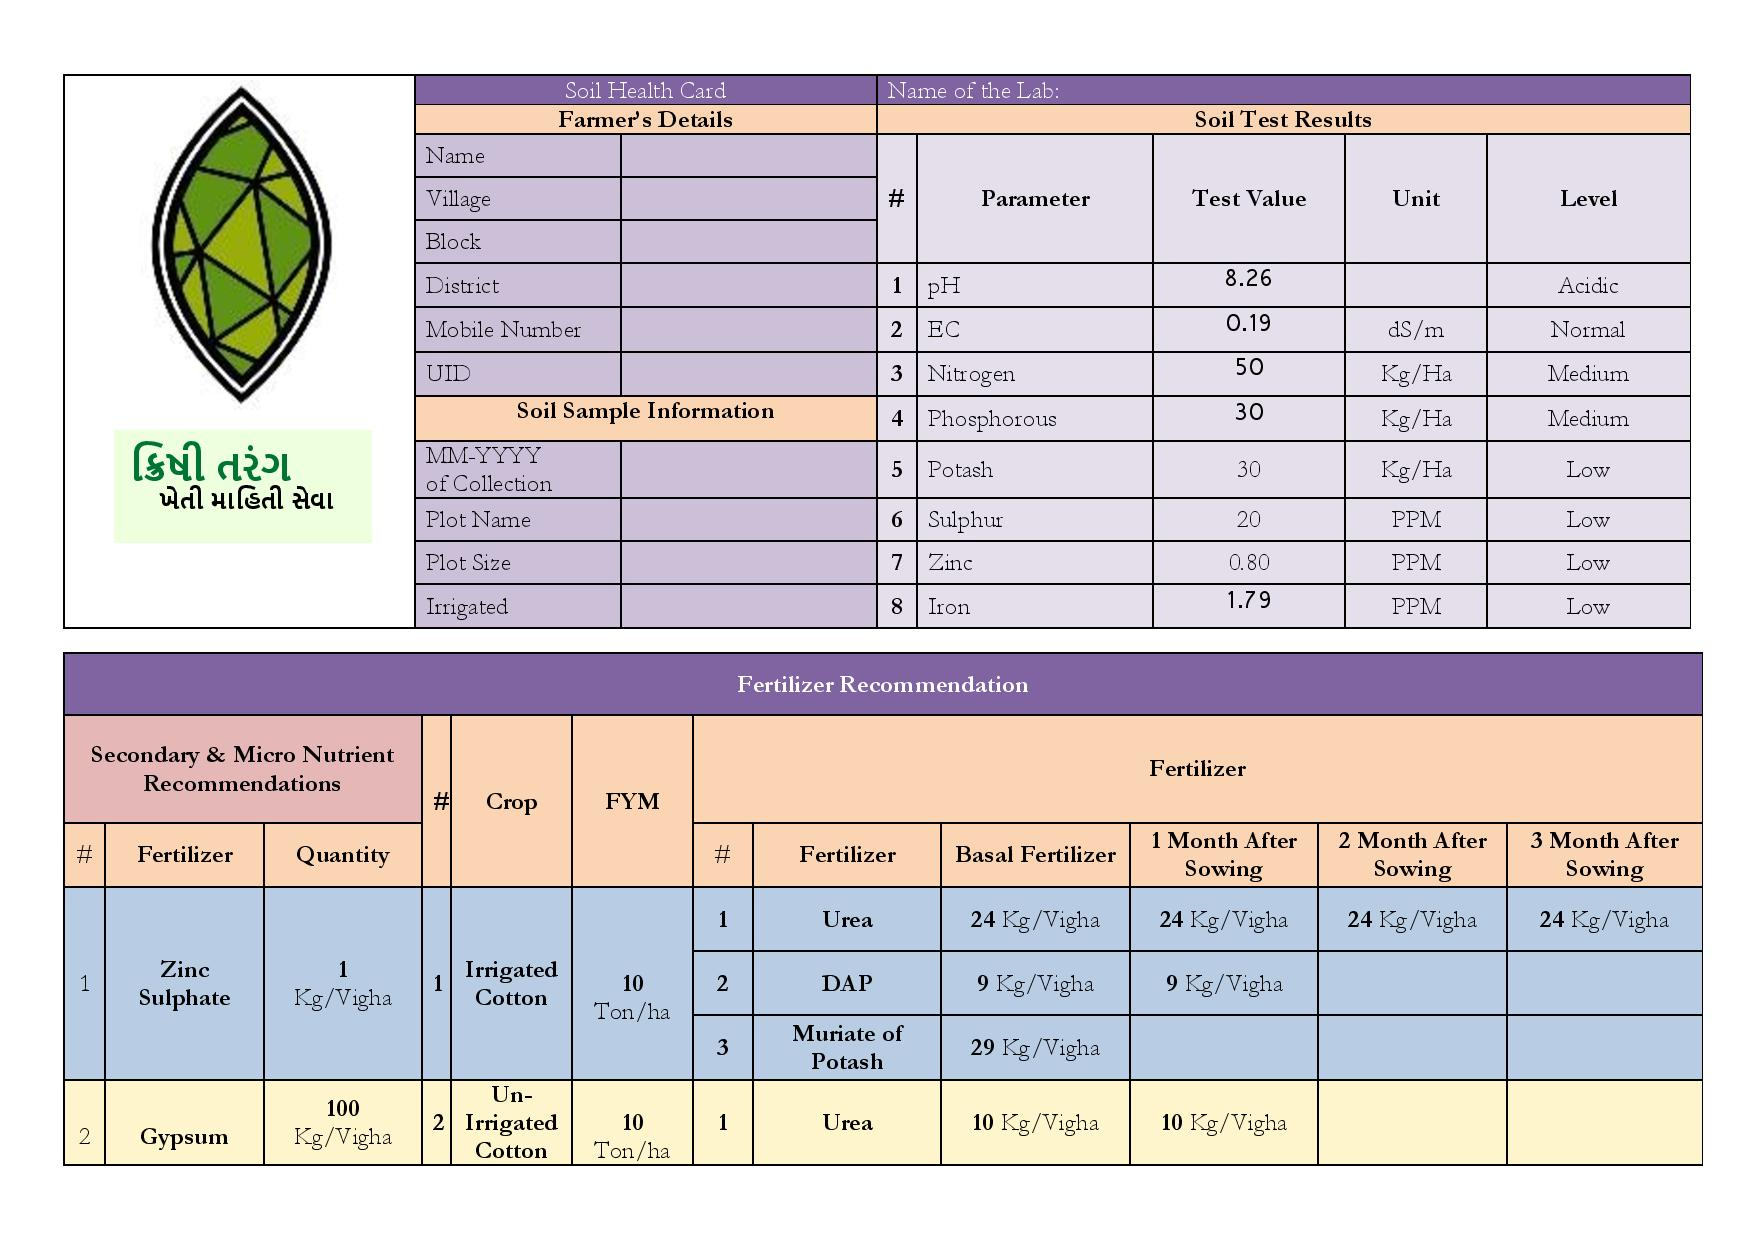
\includegraphics[width=0.9\linewidth]{figures/shc/shc} 
\end{figure}

\FloatBarrier

\pagebreak
\clearpage

\begin{figure}[!htb] \centering \caption{Supplement to Soil Health Card} \label{f:shc_supplement}
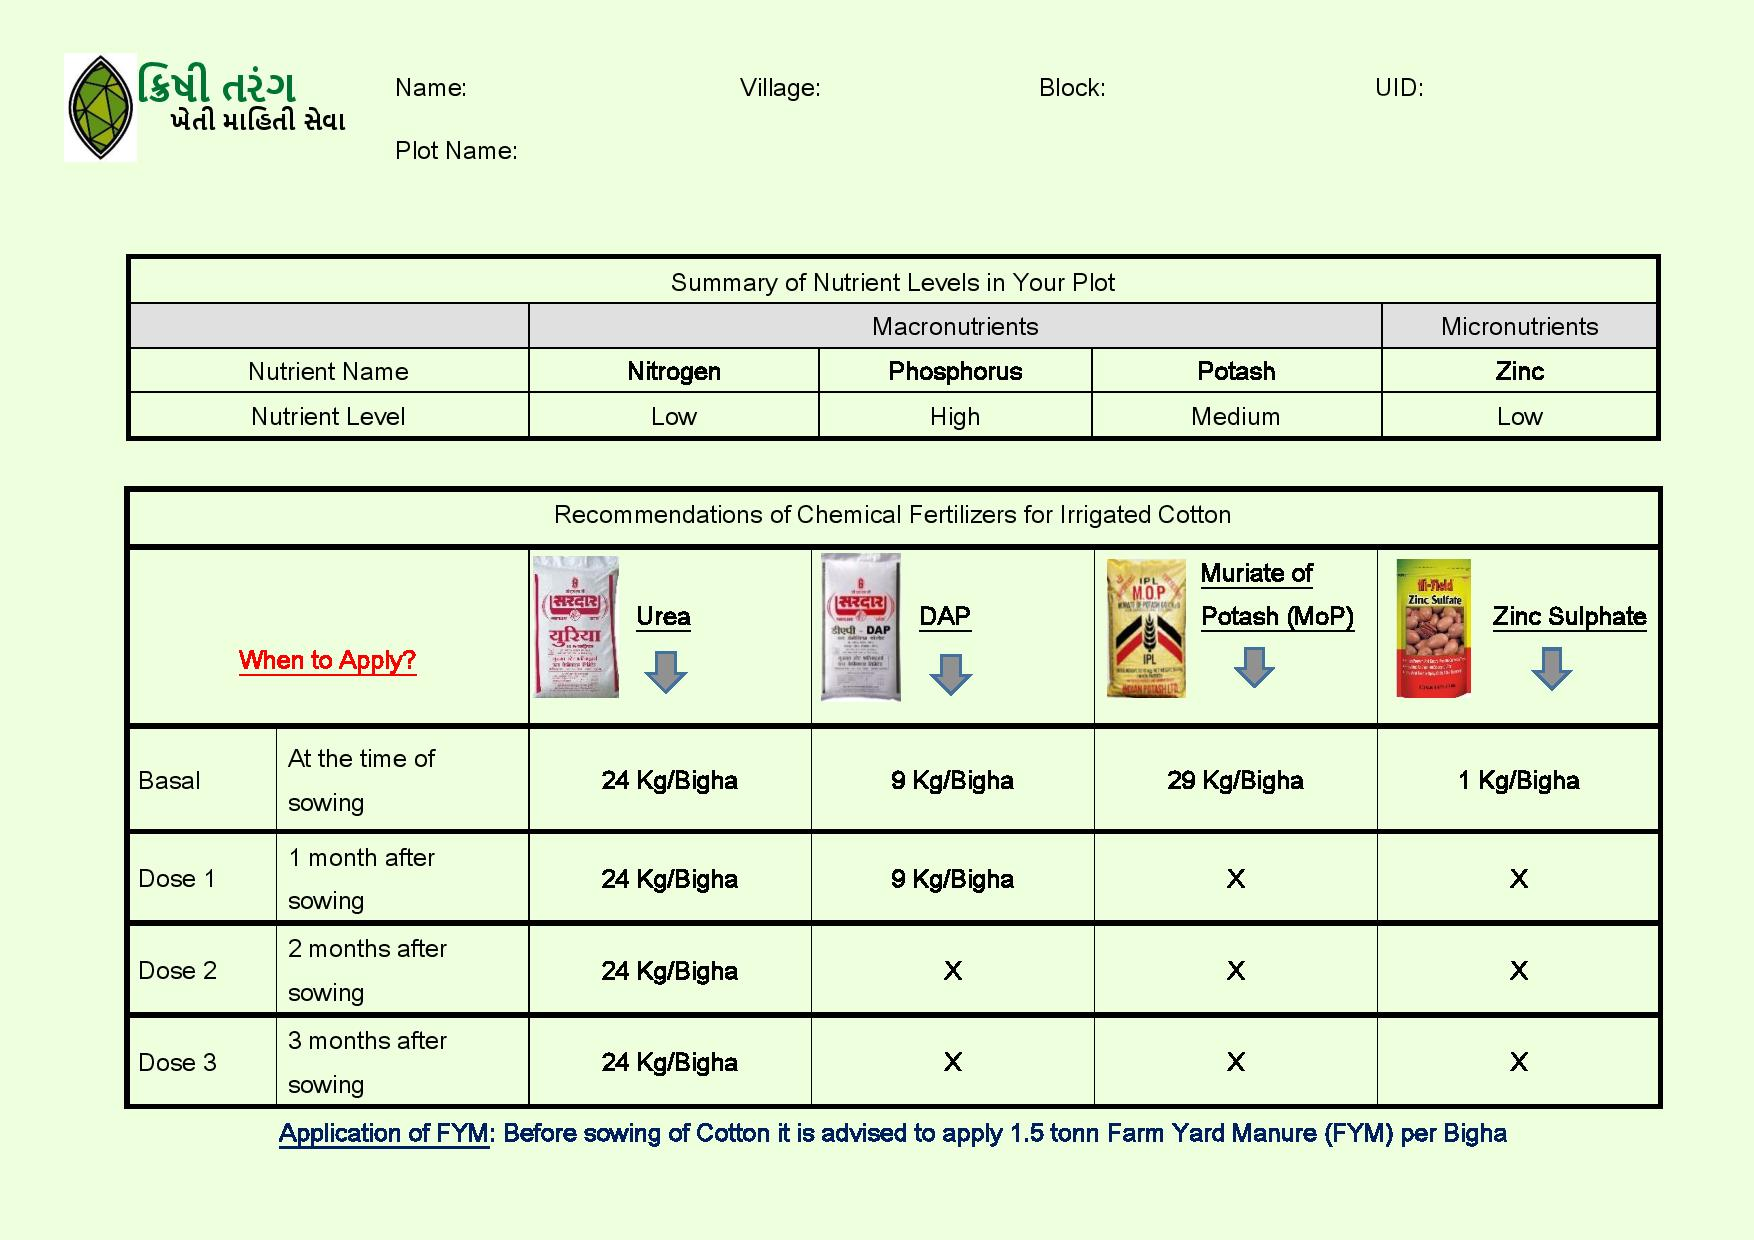
\includegraphics[width=0.9\linewidth]{figures/shc/shc_supplement} 
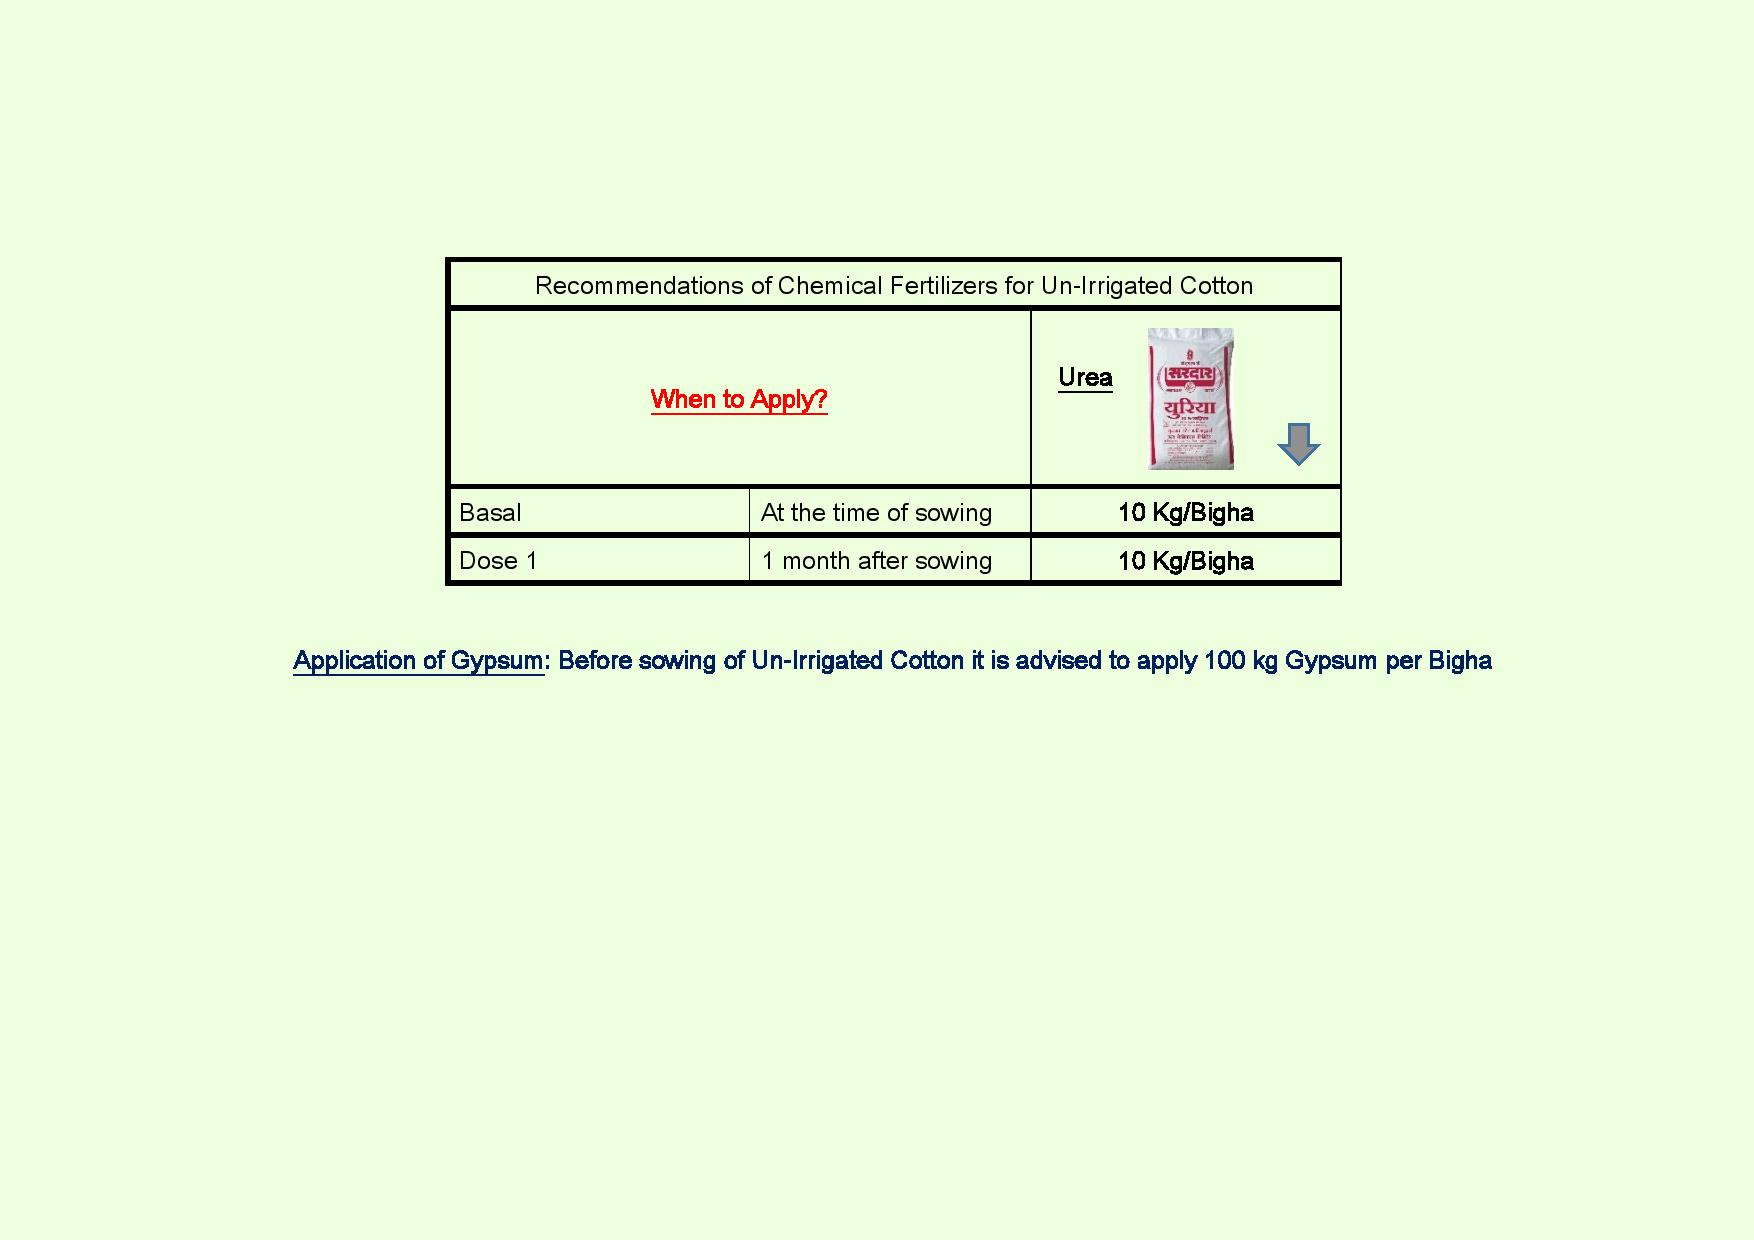
\includegraphics[width=0.9\linewidth]{figures/shc/shc_supplement_2} 
\end{figure}

\FloatBarrier

\pagebreak
\clearpage

\begin{figure}[!htb] \centering \caption{Booklet} \label{f:shc_booklet}
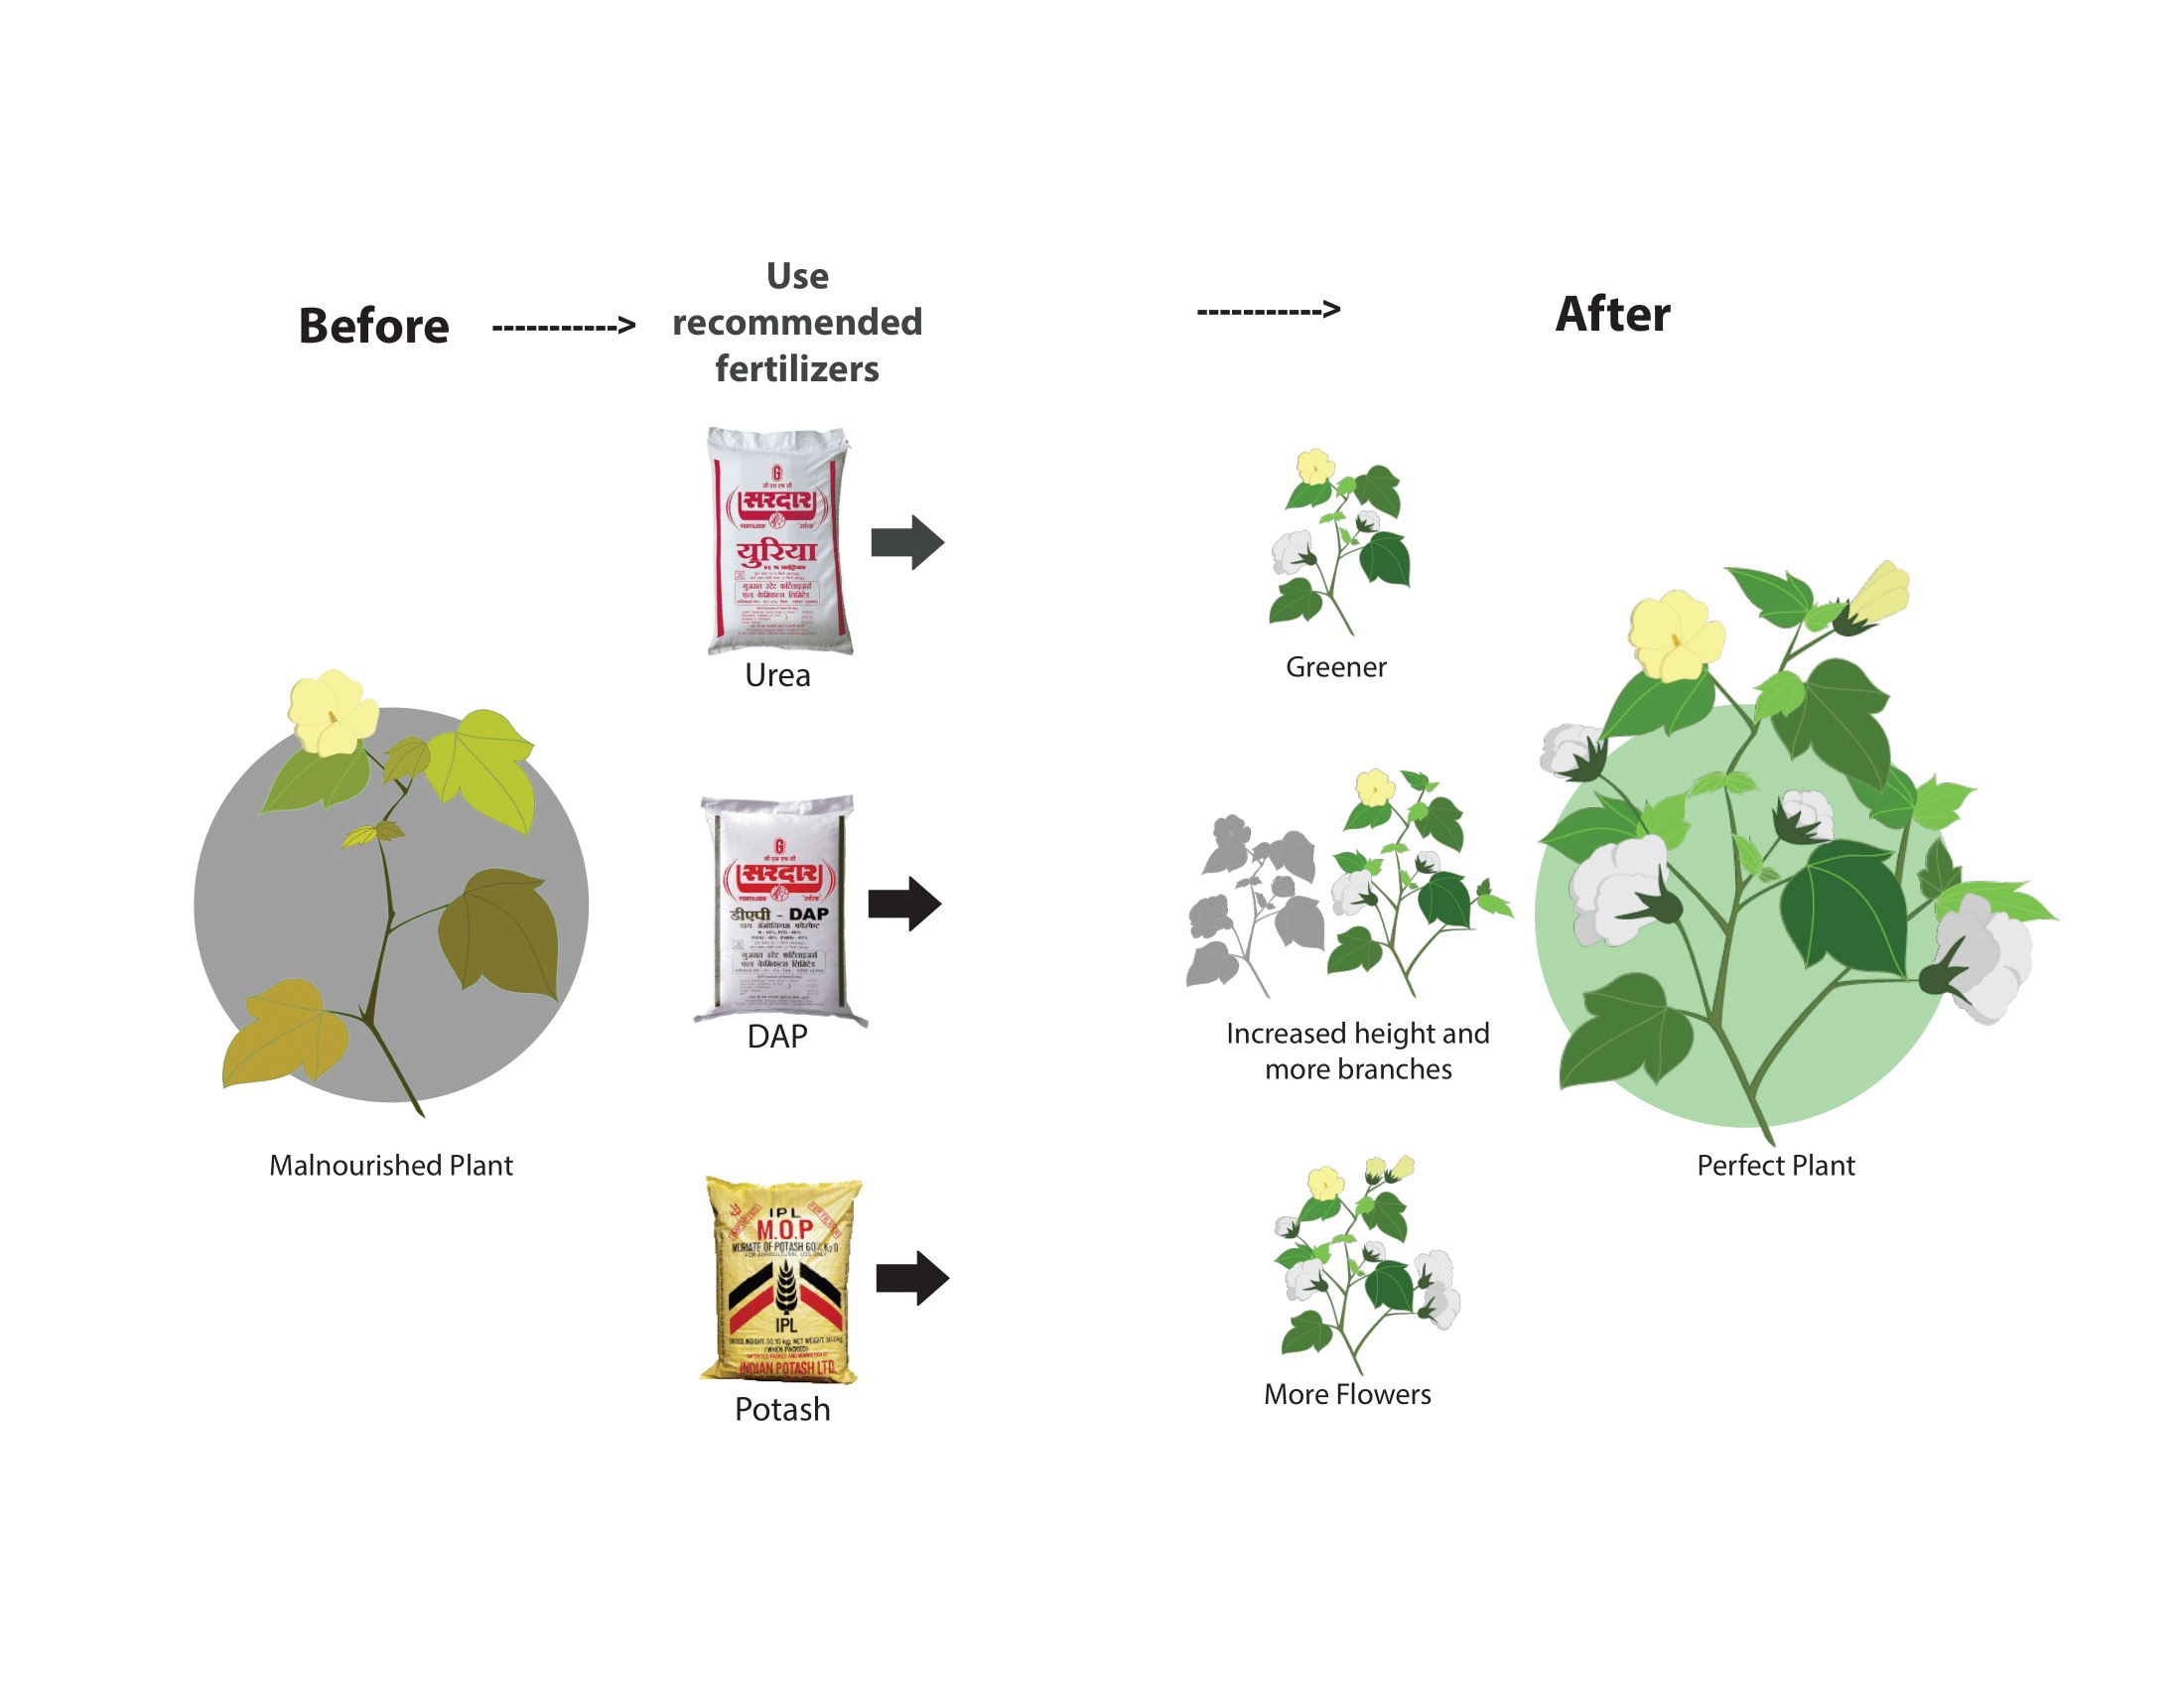
\includegraphics[width=0.9\linewidth]{figures/shc/booklet} 
\end{figure}

\FloatBarrier

\pagebreak
\clearpage

\begin{figure}[!htb] \caption{Process for calculating satellite yield measurements \\} \label{f:satellite-yield-process} \centering
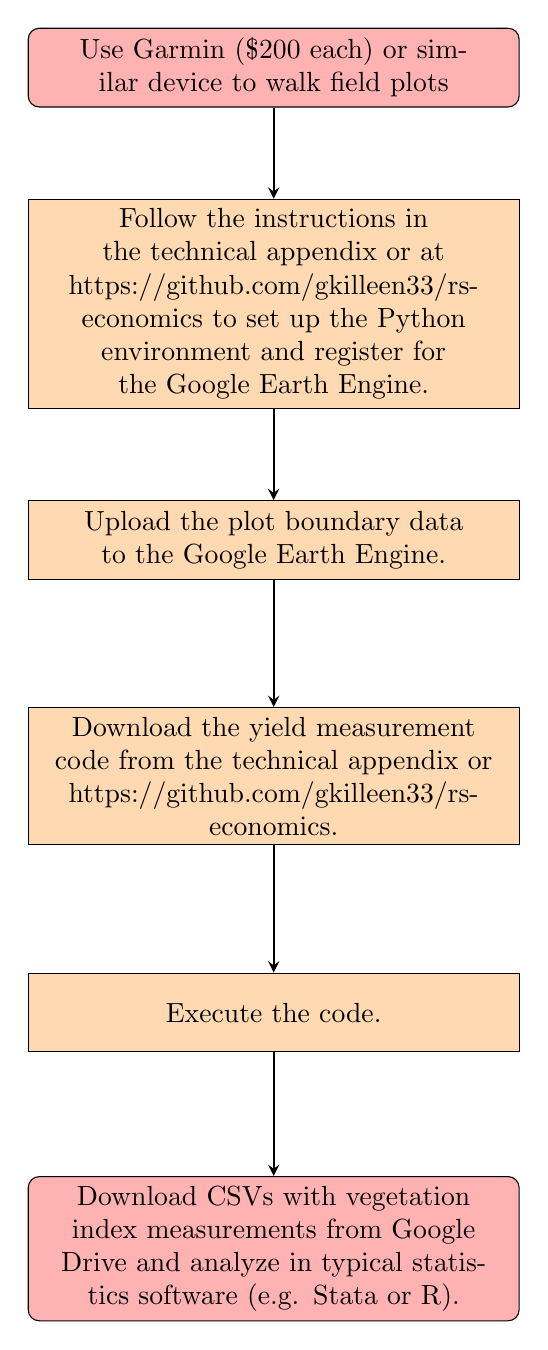
\begin{tikzpicture}[node distance=3cm]
\node (start) [startstop] {Use Garmin (\$200 each) or similar device to walk field plots};
\node (pro1) [process, below of=start] {Follow the instructions in the technical appendix or at \url{https://github.com/gkilleen33/rs-economics} to set up the Python environment and register for the Google Earth Engine.};
\node (pro2) [process, below of=pro1] {Upload the plot boundary data to the Google Earth Engine.};
\node (pro3) [process, below of=pro2] {Download the yield measurement code from the technical appendix or \url{https://github.com/gkilleen33/rs-economics}.};
\node (pro4) [process, below of=pro3] {Execute the code.};
\node (end) [startstop , below of=pro4] {Download CSVs with vegetation index measurements from Google Drive and analyze in typical statistics software (e.g. Stata or R).};
\draw [arrow] (start) -- (pro1);
\draw [arrow] (pro1) -- (pro2);
\draw [arrow] (pro2) -- (pro3);
\draw [arrow] (pro3) -- (pro4);
\draw [arrow] (pro4) -- (end);
\end{tikzpicture}
\end{figure}

\FloatBarrier

\pagebreak
\clearpage

\begin{center}
\section*{Appendix B: Tables}
\end{center}

\setcounter{table}{0}
\renewcommand{\tablename}{}\renewcommand{\thetable}{Appendix Table \arabic{table}}
\FloatBarrier

\begin{table}[!htb] \centering \caption{Generating recommendations from soil test results} \label{t:fertilizer-recommendation-methodology}
\begin{tabularx}{\linewidth}{X}
\hline \hline 
A four-step process was followed to generate customized fertilizer recommendations for each farmer: \\
1. Before the start of the agricultural season, we collected soil samples from one of the plots owned by each farmer in the sample and tested the soil samples for pH and EC and various macronutrients (nitrogen, phosphorus, potassium) and micronutrients (zinc, sulphur, iron). The soil test results contained the quantity of each nutrient in the soil and the level of each nutrient (low, medium or high).\\
2. We used nutrient levels to generate nutrient-specific recommendations. For doing so we used a template developed by Junagarh Agricultural University, in which quantities of nutrients are recommended for each of three nutrient levels. The recommended nutrient quantities for every nutrient label are the following: \\ \hline
\end{tabularx}
\begin{tabularx}{0.5\linewidth}{lXXX}
 & Low & Medium & High \\ 
Nitrogen (N) & 300 & 240 & 180 \\
Phosphorus (P) & 62.5 & 50 & 37.5 \\
Potassium (K) & 187.5 & 150 & 112.5 \\
Zinc & 25 & 20 & 15 \\
\end{tabularx}
\begin{tabularx}{\linewidth}{X}
\hline 
3. Nutrient levels were then converted to fertilizer recommendations. We focused on three macronutrients (nitrogen, phosphorus and potassium) and one micronutrient (zinc for irrigated cotton and sulphur for unirrigated cotton). \\
In irrigated plots HYV seeds are used. These seeds require adequate amounts of the three macronutrients selected, Nitrogen and phosphorus are important for crop development and potassium improves water use efficiency, builds crop resilience against certain diseases and improves fibre quality. Application of zinc was also recommended because plants from HYV seeds respond better to macronutrients when micronutrients are available in adequate quantity and most plots in the study area were deficient in this micronutrient. \\
In non-irrigated or rainfed plots, non-HYV seeds are used.  Nitrogen and sulphur were recommended because the nutrient requirements can be met with these two nutrients.\\
Our fertilizer recommendations were in terms of quantities of UREA, Di-ammonium Phosphate (DAP), Muriate of Potash (MOP), Zinc Sulphate (Zinc) and Gypsum. The table shows the nutrients contained in each fertilizer. \\ \hline 
\end{tabularx}
\begin{tabularx}{\linewidth}{lXXXXX}
 & \multicolumn{5}{c}{Nutrient content (\%)} \\
\cmidrule(l{2pt}r{2pt}){2-6} 
Fertilizer & Nitrogen & Phosphorus & Potassium & Zinc & Sulphur \\
UREA & 46 & x & x & x & x \\
DAP & 18 & 46 & x & x & x \\
MOP & x & x & 60 & x & x \\
Zinc Sulphate (Zinc) & x & x & x & 36 & 14 \\
Sulphur & x & x & x & x & 100\\
\end{tabularx}
\begin{tabularx}{\linewidth}{X}
\hline 
The nutrient levels in each fertilizer were used to calculate the exact quantity of fertilizer recommended for each plot. Our previous field surveys had shown that all the recommended fertilizers were easily available, reasonably priced and were effective for supplying nutrients to soil. \\
5. Given that fertilizers are more effective when applied in multiple small doses at various crop stages, total fertilizer recommendations were split into dose-wise recommendations. All doses contained equal quantities of fertilizer.  Following are the number of doses in which application of various nutrients is suggested: \\ \hline
\end{tabularx}
\begin{tabularx}{\linewidth}{llX|lX}
 & \multicolumn{2}{c}{Irrigated Crop} & \multicolumn{2}{c}{Un-irrigated crop} \\
\cmidrule(l{2pt}r{2pt}){2-3} \cmidrule(l{2pt}r{2pt}){4-5} 
 & Number of doses & Timing of doses & Number of doses & Timing of doses \\
Nitrogen & 4 & \makecell[l]{- At time of sowing (basal dose) \\ - One month after sowing \\ - Two months after sowing \\ - Three months after sowing} & 2 & \makecell[l]{- At time of sowing (basal dose) \\ - One month after sowing} \\
Phosphorus & 2 & \makecell[l]{- At time of sowing (basal dose) \\ - One month after sowing} & 0 & \\
Potassium & 1 & - At time of sowing (basal dose) & 0 & \\
Zinc & 1 & - At time of sowing (basal dose) & 0 & \\
Sulphur & 1 & - At time of sowing (basal dose) & 1 & - At time of sowing (basal dose)
\end{tabularx}
\begin{tabularx}{\linewidth}{X}
\hline 
Fertilizer and nutrient recommendations were generated for ‘per unit of area’ to make recommendations farmer friendly. This means that the recommendations were generated for the area unit  in which a farmer had reported crop area at baseline. For example, if a farmer had reported land in acre, then customized fertilizer recommendations were made in per acre terms. Also, since irrigation status of crops is uncertain for farmers in India at the start of the agricultural season, recommendations for both irrigated and unirrigated cotton were generated for each farmer.  \\ 
\end{tabularx}
\end{table}

\FloatBarrier

\pagebreak
\clearpage

\FloatBarrier

\begin{table}[!htb] \centering \caption{Fertilizer knowledge questions} \label{t:knowledge-questions}
\begin{tabularx}{\linewidth}{lXX}
\hline \hline 
 & Question & Correct Answer \\
\hline
1. & Which main nutrients are required by irrigated cotton for growth? & Nitrogen, Phosphorous, and Potash \\ [1em]
2. & Which of the following is main nutrient in UREA? & Nitrogen \\ [1em]
3. & Which of the following is main nutrient in DAP? & Phosphorous \\ [1em]
4. & Which of the following is main nutrient in MOP? & Potash \\ [1em]
5. & Which is the best fertilizer for applying nitrogen in the soil? & UREA \\ [1em]
6. & Which is the best fertilizer for adding potash in the soil? & MOP \\ [1em]
7. & When is zinc recommended to be applied during cotton cultivation for irrigated cotton? & At the time of sowing \\ [1em]
8. & When should Urea be applied in the soil for irrigated cotton? & At time of sowing, and 1, 2, and 3 months after sowing \\ [1em]
9. & When should Urea be applied in the soil for un-irrigated cotton? & At the time of sowing and one month after sowing \\ [1em]
10. & When should DAP be applied in the soil for cotton cultivation? & At the time of sowing, and one month after sowing \\ [1em]
11. & When should MoP be applied in the soil for cotton cultivation? & At the time of sowing \\ [1em]
12. & What is the benefit of appling UREA to soil? & More green \\ [1em]
13. & What is the benefit of applying DAP to soil? & Increased height and more branches \\ [1em]
14. & What is the benefit of applying Potash to soil? & More flowers \\ 
\hline
\end{tabularx}
\end{table}

\FloatBarrier

\pagebreak
\clearpage

\FloatBarrier

\begin{table}[!htb] \centering \caption{Survey completion rates} \label{t:survey-completion-rates}
\begin{tabular}{lrrrrrr}
\hline \hline 
\\[-2mm]
 & \multicolumn{2}{c}{\textbf{Control}} & \multicolumn{2}{c}{\textbf{Treatment}} & \multicolumn{2}{c}{\textbf{Total}} \\
\cmidrule(l{.75em}){2-3} \cmidrule(l{.75em}){4-5}\cmidrule(l{.75em}){6-7}
&Number&Percent&Number&Percent&Number&Percent \\
\midrule
\textbf{Grew cotton}&&&&&& \\
Did not sow cotton&45&5.7&38&4.8&83&5.2 \\
Sowed cotton&745&94.3&754&95.2&1499&94.8 \\
\textbf{Total}&790&100.0&792&100.0&1582&100.0 \\
\midrule
\textbf{Basal}&&&&&& \\
Completed basal survey&707&89.3&729&91.9&1436&90.6 \\
Attrited&85&10.7&64&8.1&149&9.4 \\
\textbf{Total}&792&100.0&793&100.0&1585&100.0 \\
\midrule
\textbf{Midline}&&&&&& \\
Completed midline survey&773&97.6&760&95.8&1533&96.7 \\
Attrited&19&2.4&33&4.2&52&3.3 \\
\textbf{Total}&792&100.0&793&100.0&1585&100.0 \\
\midrule
\textbf{Endline}&&&&&& \\
Completed endline survey&736&92.9&729&91.9&1465&92.4 \\
Attrited&56&7.1&64&8.1&120&7.6 \\
\textbf{Total}&792&100.0&793&100.0&1585&100.0 \\
\midrule
\textbf{Missing plot map}&&&&&& \\
Plot mapped&702&88.6&687&86.6&1389&87.6 \\
Plot not mapped&90&11.4&106&13.4&196&12.4 \\
\textbf{Total}&792&100.0&793&100.0&1585&100.0 \\
\midrule
\textbf{All surveys and mapping complete}&&&&&& \\
Did not complete 1+ surveys&168&21.2&175&22.1&343&21.6 \\
Completed all surveys&624&78.8&618&77.9&1242&78.4 \\
\textbf{Total}&792&100.0&793&100.0&1585&100.0 \\

\hline
\multicolumn{7}{@{}m{6in}@{}}{\footnotesize \ref{t:survey-completion-rates} presents the completion rate of each survey and the plot mapping exercise. We determined that a farmer completed a given survey if they grew cotton, the surveyor was able to conduct the survey, and the farmer consented to be surveyed. In two instances, farmers attempted to grow cotton but the crops failed extremely early in the season. We treated these two observations as if the farmers did not grow cotton since they did not apply any inputs.}
\end{tabular}
\end{table}

\FloatBarrier

\pagebreak
\clearpage

\FloatBarrier

\begin{table} \centering \caption{Attrition} \label{t:attrition}
\def\sym#1{\ifmmode^{#1}\else\(^{#1}\)\fi}
\begin{tabularx}{\linewidth}{@{}XSSSSS@{}}
\hline\hline
&\multicolumn{1}{c}{(1)}&\multicolumn{1}{c}{(2)}&\multicolumn{1}{c}{(3)}&\multicolumn{1}{c}{(4)}&\multicolumn{1}{c}{(5)}\\
&\multicolumn{1}{c}{Basal}&\multicolumn{1}{c}{Midline}&\multicolumn{1}{c}{Endline}&\multicolumn{1}{c}{\makecell[c]{Farmer-reported \\ yield}}&\multicolumn{1}{c}{\makecell[c]{Satellite \\ data}}\\
\hline
\\[-2mm]
\partialinput{4}{51}{tables/t-a2/attrition.tex} 
\partialinput{57}{61}{tables/t-a2/attrition.tex}
\hline
\multicolumn{6}{@{}m{\textwidth}@{}}{\footnotesize Robust standard errors in parentheses. \sym{*} \(p<0.10\), \sym{**} \(p<0.05\), \sym{***} \(p<0.01\)} \\
\multicolumn{6}{@{}m{\textwidth}@{}}{\footnotesize \ref{t:attrition} reports the results of tests for differential attrition. Each regression includes interactions between treatment and each other independent variable which are omitted for space. We present the results of an F-test evaluating the joint significance of the interaction terms. A survey is defined as complete if the farmer consented to be interviewed and sowed cotton. Education data was missing for 175 observations. Number of children is missing for 25 observations. Crop insurance is missing for 20 observations. UREA and DAP usage last season are missing for 3 observations, DAP and MOP usage last season are missing for two observations, and sampled plot size is missing for one observations. Missing values of these variables were imputed with the median value of each variable. All regressions include block fixed effects.}
\end{tabularx}
\end{table}

\FloatBarrier

\pagebreak
\clearpage

\begin{table}[!ht] \centering \caption{Listening rates of treatment calls \\ Administrative data} \label{t:treatment-call-listening-rates}
\begin{tabular}{lcc}
\hline \hline 
                    &\makecell[c]{Share of relevant farmers \\ that heard $\ge$ 1 call}&Number of relevant farmers\\
\hline
Basal: irrigated (UREA, MOP, and DAP)&       0.883&         529\\
Early season: Potash (irrigated)&       0.866&         529\\
Dose 2: irrigated (UREA, MOP, and DAP)&       0.820&         529\\
Dose 3: irrigated (UREA, MOP, and DAP)&       0.788&         529\\
Dose 4: irrigated (UREA, MOP, and DAP)&       0.745&         529\\
Early season: Potash (irrigated)&       0.866&         529\\
Mid-season: Potash (irrigated)&       0.713&         529\\
Early season: Zinc (irrigated)&       0.758&         529\\
Mid-season: Zinc (irrigated)&       0.437&         529\\
Basal: unirrigated (UREA)&       0.760&         225\\
Dose 2: unirrigated (UREA)&       0.729&         225\\

\hline
\multicolumn{3}{@{}m{6in}@{}}{\footnotesize \ref{t:treatment-call-listening-rates} reports the share and number relevant farmers in the treatment group that heard at least 1 customized fertilizer recommendation of the indicated type. A relevant farmer means that they sowed cotton and have an irrigated plot if the advice is for irrigated plots or an unirrigated plot if the recommendation is for unirrigated plots. Customized calls were only sent to farmers in the treatment group. All treatment farmers received the same calls. If the call duration exceeded the point where a recommendation was given, then heard recommendation was assigned a value of 1. The last two rows have a smaller sample size because the majority of farmers reported growing irrigated cotton.}
\end{tabular}
\end{table}

\FloatBarrier

\begin{table}[!ht] \centering \caption{Treatment effect on basal fertilizer usage \\ Basal survey} \label{t:fertilizer-use-basal-detailed}
\def\sym#1{\ifmmode^{#1}\else\(^{#1}\)\fi}
\begin{tabularx}{\linewidth}{@{}XZZZZZ@{}}
\hline \hline 
\\[-2mm]
&\multicolumn{1}{c}{(1)}&\multicolumn{1}{c}{(2)}&\multicolumn{1}{c}{(3)}&\multicolumn{1}{c}{(4)}&\multicolumn{1}{c}{(5)}\\
&\multicolumn{1}{c}{UREA}&\multicolumn{1}{c}{DAP}&\multicolumn{1}{c}{MOP}&\multicolumn{1}{c}{Zinc}&\multicolumn{1}{c}{\makecell[c]{Standardized \\ joint effect}}\\
\hline 
\\[-2mm]
\multicolumn{6}{l}{\textit{Panel A: Binary fertilizer decision consistent with recommendation}} \\ [1em]
\partialinput{4}{5}{tables/t-a4/followed_rec_basal} [1em]
\partialinput{9}{12}{tables/t-a4/followed_rec_basal}
\end{tabularx}
\begin{tabularx}{\linewidth}{@{}XZZZZZ@{}}
\\[-2mm]
\multicolumn{6}{l}{\textit{Panel B: Amount of fertilizer applied (kg/ha)}} \\ [1em]
\partialinput{4}{5}{tables/t-a4/fert_applied_basal} [1em]
\partialinput{9}{12}{tables/t-a4/fert_applied_basal}
\end{tabularx}
\begin{tabularx}{\linewidth}{@{}XZZZZZ@{}}
\\[-2mm]
\multicolumn{6}{l}{\textit{Panel C: Distance between suggested and applied fertilizer (kg/ha)}} \\ [1em]
\partialinput{4}{5}{tables/t-a4/gap_basal.tex} [1em]
\partialinput{9}{12}{tables/t-a4/gap_basal.tex}
\hline
\multicolumn{6}{@{}m{\linewidth}@{}}{\footnotesize Robust standard errors in parenthesis. \sym{*} \(p<0.10\), \sym{**} \(p<0.05\), \sym{***} \(p<0.01\)} \\
\multicolumn{6}{@{}m{\linewidth}@{}}{\footnotesize This table reports fertilizer application information for the basal (first) dose, which was emphasized in the advisory messages. In panel (a), the dependent variable is assigned a value of 1 if the farmer applied the indicated fertilizer type and was advised to, or did not apply the fertilizer type and was advised not to. The variable is coded to 0 if the farmer did not follow recommendations. In panel (b), the dependent variable is the amount of fertilizer the respondent reported applying during the basal dose in kilograms divided by the area on which they applied the fertilizer in hectare. Panel (c) report regressions of the absolute value of the difference between the recommended and applied fertilizer amount in kg/ha. Differences are winsorized at the 99th percentile. In each panel, column (5) reports the average standardized effect across columns (1) - (4), which is an equally-weighted sum across the standardized treatment effects on the outcome for each input type.}
\end{tabularx}
\end{table}

\FloatBarrier

\pagebreak
\clearpage

\FloatBarrier

\begin{table}[!ht] \centering \caption{Treatment effect on full season fertilizer use \\ Midline survey} \label{t:fertilizer-use-midline-detailed}
\def\sym#1{\ifmmode^{#1}\else\(^{#1}\)\fi}
\begin{tabularx}{\linewidth}{@{}XSSSSS@{}}
\hline \hline 
\\[-2mm]
&\multicolumn{1}{c}{(1)}&\multicolumn{1}{c}{(2)}&\multicolumn{1}{c}{(3)}&\multicolumn{1}{c}{(4)}&\multicolumn{1}{c}{(5)}\\
&\multicolumn{1}{c}{\makecell[c]{UREA}}&\multicolumn{1}{c}{\makecell[c]{DAP}}&\multicolumn{1}{c}{\makecell[c]{MOP}}&\multicolumn{1}{c}{\makecell[c]{Zinc}}&\multicolumn{1}{c}{\makecell[c]{Standardized \\ joint effect}}\\
& & & & & \\[-3mm]
\hline
\end{tabularx}
\begin{tabularx}{\linewidth}{@{}XSSSSS@{}}
\\[-2mm]
\multicolumn{6}{l}{\textit{Panel A: Total amount of fertilizer applied (kg/ha)}} \\ [1em]
\partialinput{4}{5}{tables/t-a6/fert_applied_midline.tex} [1em]
\partialinput{9}{12}{tables/t-a6/fert_applied_midline.tex}
\end{tabularx}
\begin{tabularx}{\linewidth}{@{}XSSSSS@{}}
\\[-2mm]
\multicolumn{6}{l}{\textit{Panel B: Distance between suggested and applied fertilizer (kg/ha)}} \\ [1em]
\partialinput{4}{5}{tables/t-a6/gap_all_doses.tex} [1em]
\partialinput{9}{12}{tables/t-a6/gap_all_doses.tex}
\hline
\multicolumn{6}{@{}m{\linewidth}@{}}{\footnotesize Robust standard errors in parenthesis. \sym{*} \(p<0.10\), \sym{**} \(p<0.05\), \sym{***} \(p<0.01\)} \\
\multicolumn{6}{@{}m{\linewidth}@{}}{\footnotesize Panel (a) reports the total amount of fertilizer the respondent applied across all doses divided by the average area on which the respondent reported applying fertilizer in kilograms. Panel (b) report regressions of the absolute value of the difference between the recommended and applied fertilizer amount in kg/ha. We use GPS plot area data where available, and otherwise use farmer-reported plot size. Differences are winsorized at the 99th percentile. The last column in panels (a) and (b) reports the average standardized effect across each of the other columns, which is an equally-weighted sum across the standardized treatment effects on the outcome for each input type. }
\end{tabularx}
\end{table}

\FloatBarrier

\pagebreak
\clearpage

\FloatBarrier

\begin{table}[!ht] \centering \caption{Average plot share on which fertilizer was applied \\ Conditional on applying fertilizer \\ Basal and midline surveys} \label{t:fertilizer-share}
\def\sym#1{\ifmmode^{#1}\else\(^{#1}\)\fi}
\begin{tabularx}{0.5\linewidth}{@{}XZZ@{}}
\hline \hline 
\\[-2mm]
&\multicolumn{1}{c}{(1)}&\multicolumn{1}{c}{(2)}\\
&\multicolumn{1}{c}{\makecell[c]{Control}}&\multicolumn{1}{c}{\makecell[c]{Treatment}}\\
\hline
\\[-2mm]
\multicolumn{3}{l}{\textit{Panel A: Basal dose}} \\ [1em]
UREA &     1.000 &     1.000 \\ 
 & [0.000] & [0.000] \\ 
 & N:        49 & N:       130 \\ [1em] 
DAP &     0.999 &     0.999 \\ 
 & [0.012] & [0.018] \\ 
 & N:       440 & N:       491 \\ [1em] 
MOP &     1.000 &     1.000 \\ 
 & [0.000] & [0.000] \\ 
 & N:        16 & N:        89 \\ [1em] 
Zinc &     1.000 &     1.000 \\ 
 & [0.000] & [0.000] \\
 & N:         4 & N:        26 \\ 
 
\end{tabularx}
\begin{tabularx}{0.5\linewidth}{@{}XZZ@{}}
\\[-2mm]
\multicolumn{3}{l}{\textit{Panel B: Average across all doses}} \\ [1em]
UREA &     0.999 &     0.999 \\ 
 & [    0.022] & [    0.027] \\ 
 & N:       596 & N:       620 \\ [1em] 
DAP &     1.000 &     0.999 \\ 
 & [    0.010] & [    0.023] \\ 
 & N:       587 & N:       588 \\ [1em] 
MOP &     0.982 &     1.000 \\ 
 & [    0.094] & [    0.000] \\ 
 & N:        55 & N:       160 \\ [1em] 
Zinc &     1.000 &     1.000 \\ 
 & [    0.000] & [    0.000] \\ 
 & N:        37 & N:        66 \\ 

\hline
\multicolumn{3}{@{}m{0.5\linewidth}@{}}{\footnotesize \ref{t:fertilizer-share} presents the share of farmers' plots on which each fertilizer type was applied. Observations for which a given fertilizer type was not applied are excluded. Panel (a) reports plot shares at the basal dose. Panel (b) reports the average plot share reported across all doses. Standard deviations are included in brackets.}
\end{tabularx}
\end{table}

\FloatBarrier

\pagebreak
\clearpage

\FloatBarrier

\begin{table}[!htb] \centering \caption{Satellite data availability \\ GPS and Sentinel-2 data} \label{t:sentinel-attrition}
\begin{tabularx}{5.5in}{@{}Xrrrrrr@{}}
\hline \hline 
\\[-2mm]
 & \multicolumn{2}{c}{Control} & \multicolumn{2}{c}{Treatment} & \multicolumn{2}{c}{Total} \\
\cmidrule(l{.75em}){2-3} \cmidrule(l{.75em}){4-5}\cmidrule(l{.75em}){6-7}
&Number&Percent&Number&Percent&Number&Percent \\
\hline 
\\[-2mm]
\multicolumn{7}{l}{\textit{Plot mapping}} \\ 
\partialinput{8}{9}{tables/t-b1/sentinel-attrition.tex} [1em]
\multicolumn{7}{l}{\textit{Sentinel-2: 2016}} \\ 
\partialinput{12}{13}{tables/t-b1/sentinel-attrition.tex} [1em]
\multicolumn{7}{l}{\textit{Sentinel-2: 2017}} \\ 
\partialinput{16}{17}{tables/t-b1/sentinel-attrition.tex} [1em]
\multicolumn{7}{l}{\textit{Sentinel-2: 2018}} \\ 
\partialinput{20}{20}{tables/t-b1/sentinel-attrition.tex} [1em]
\multicolumn{7}{l}{\textit{Sentinel-2: no missing data}} \\ 
\partialinput{23}{24}{tables/t-b1/sentinel-attrition.tex}
\hline
\multicolumn{7}{@{}m{5.5in}@{}}{\footnotesize \ref{t:sentinel-attrition} reports the availability of cloud-free Sentinel-2 satellite imagery by treatment status. Data is non-missing for a plot in a year if at least one cloud free image was available. There is no data available for 3 plots in 2016 and 2017 because they fall outside of the Sentinel-2 swath that images the majority of the sample.}
\end{tabularx}
\end{table}

\FloatBarrier

\pagebreak
\clearpage

\FloatBarrier

\begin{table}[!ht] \centering \small 
\caption{Vegetation indices} \label{indices} 
\begin{tabular}{l c c l} 
\hline \hline 
\\ [-2ex]
Index & Equation & \makecell{Equation in \\ Sentinel-2 bands} & Source \\ 
\hline 
\\ [-1ex]
\makecell[l]{Normalized Difference \\ Vegetation Index (NDVI)} & $\dfrac{NIR-Red}{NIR+Red}$ & $\dfrac{B8-B4}{B8+B4}$ & \citet{Haas1974MonitoringERTS} \\ [3ex]
\makecell[l]{Green Chlorophyll Vegetation \\ Index (GCVI)} & $\left( \dfrac{NIR}{GREEN} \right) - 1$ & $\left(\dfrac{B8}{B3} \right) -1$ & \citet{Gitelson2003RemoteCanopies} \\ [3ex]
Red-edge NDVI (reNDVI) & $\dfrac{NIR-RE}{NIR+RE}$ & $\dfrac{B8-B5}{B8+B5}$ & \citet{Vina2005NewCrops} \\ [3ex]
\makecell[l]{MERIS Terrestrial Chlorophyll \\ Index (MTCI)} & $\dfrac{NIR-RE}{RE-Red}$ & $\dfrac{B8-B5}{B5-B4}$ & \citet{Dash2004TheIndex}  \\ [3ex]
\makecell[l]{Leaf Area Index (LAI)} & Neural net & \citet{Weiss2016S2ToolBoxFCOVER} & \citet{Weiss1999EvaluationData} \\ [2ex]
\hline 
\\ [-2ex]
\multicolumn{4}{@{}m{0.75\linewidth}@{}}{\footnotesize Sentinel-2 bands 3, 4, and 8 have a 10 meter by 10 meter resolution, but band 5 has a 20 meter by 20 meter resolution. Hence, we resampled band 5 using a bilinear algorithm before deriving the Red-edge NDVI and MTCI. We resampled all Sentinel-2 bands to 10 meters before calculating LAI.}
\end{tabular}
\end{table}

\FloatBarrier

\pagebreak
\clearpage

\FloatBarrier

\begin{table}[!ht] \centering \caption{Satellite-measured vs farmer-reported yields \\ Endline survey, GPS data, and Sentinel-2 imagery} \label{b:fr-vs-satellite-yield-plot-size}
\def\sym#1{\ifmmode^{#1}\else\(^{#1}\)\fi}
\begin{tabularx}{\linewidth}{@{}XSSSSS@{}}
\hline \hline 
\\[-2mm]
&\multicolumn{1}{c}{(1)}&\multicolumn{1}{c}{(2)}&\multicolumn{1}{c}{(3)}&\multicolumn{1}{c}{(4)}&\multicolumn{1}{c}{(5)}\\
&\multicolumn{1}{c}{NDVI}&\multicolumn{1}{c}{GCVI}&\multicolumn{1}{c}{reNDVI}&\multicolumn{1}{c}{MTCI}&\multicolumn{1}{c}{LAI}\\
\hline
\\[-2mm]
\multicolumn{6}{l}{\textit{Panel A: Plots above the median size}} \\ [1em]
\partialinput{4}{8}{tables/t-b3/above_median.tex} [1em]
\partialinput{10}{12}{tables/t-b3/above_median.tex}
\end{tabularx}
\begin{tabularx}{\linewidth}{@{}XSSSSS@{}}
\\[-2mm]
\multicolumn{6}{l}{\textit{Panel B: Plots below the median size}} \\ [1em]
\partialinput{4}{8}{tables/t-b3/below_median.tex} [1em]
\partialinput{10}{13}{tables/t-b3/below_median.tex}
\hline
\multicolumn{6}{@{}m{\linewidth}@{}}{\footnotesize Robust standard errors in parenthesis. \sym{*} \(p<0.10\), \sym{**} \(p<0.05\), \sym{***} \(p<0.01\)} \\
\multicolumn{6}{@{}m{\linewidth}@{}}{\footnotesize \ref{b:fr-vs-satellite-yield-plot-size} reports the results of regressions of satellite vegetation indices (VIs), calculated using Sentinel-2 L2A multispectral satellite imagery, on farmer reported productivity. We calculated the median VI value observed in each plot for 5 Sentinel-2 images from 2018 and then took the maximum value across the 5 satellite passes for each plot and each VI. We removed outlying observations in farmer-reported data by winsoring strictly positive values at the 2nd and 98th percentiles. We report the probability that the increase in adjusted $R^2$ from panel (a) to panel (b) is due to random chance in each column. These p-values were obtained using randomization inference.}
\end{tabularx}
\end{table}

\FloatBarrier

\pagebreak
\clearpage

\FloatBarrier

\begin{table}[!ht] \centering \caption{The effect of irrigation on yields (kilograms/hectare) \\ Survey data, GPS data, and Sentinel-2 imagery} \label{b:fr-vs-satellite-irrigation}
\def\sym#1{\ifmmode^{#1}\else\(^{#1}\)\fi}
\begin{tabularx}{\linewidth}{@{}XZZZ@{}}
\hline \hline 
\\[-2mm]
\partialinput{1}{14}{tables/t-b4/irrigation.tex} [1em]
\partialinput{16}{19}{tables/t-b4/irrigation.tex}
\hline
\multicolumn{4}{@{}m{\linewidth}@{}}{\footnotesize Clustered standard errors in parenthesis. \sym{*} \(p<0.10\), \sym{**} \(p<0.05\), \sym{***} \(p<0.01\)} \\
\multicolumn{4}{@{}m{\linewidth}@{}}{\footnotesize \ref{b:fr-vs-satellite-irrigation} compares regressions of farmer-reported yields and satellite-measured yields on year dummies, irrigation status, and an interaction between irrigation status and year. In column (1), the dependent variable is farmer-reported total cotton yield, in kilograms, divided by cultivation area, in hectares. In columns (2) and (3), the dependent variable is satellite-measured productivity. We calculated satellite-measured yield by calculating, from Sentinel-2 imagery, the median Red-edge NDVI (reNDVI) pixel value observed in each plot for each satellite pass. We then linearly transformed the reNDVI values to productivity using a linear regression on farmer-reported yield divided by GPS-measured plot size. Column (2) uses Sentinel-2 observations from October 28, 2017 and October 28, 2018 only. Column (3) includes all 2017 and 2018 Sentinel-2 passes that we analyze in this paper. Irrigation is defined as 1 if the farmer reported irrigating their plot using underground water, a nearby water source/dam, or a canal during the baseline survey. In 491 instances, farmers indicated that they had an irrigation system fed by rainfall. We coded irrigation to 0 in these cases since the variable is intended to capture whether the respondent has an irrigation system independent of rainfall. We removed outlying observations in farmer-reported yield data by winsoring strictly positive values at the 2nd and 98th percentiles. The sample is restricted to observations for which none of the dependent variables are missing.}
\end{tabularx}
\end{table}

\FloatBarrier

\clearpage
\pagebreak

\newgeometry{top=1in,bottom=1in,left=1in,right=1in}

\section{Technical Appendix} \label{technical-appendix}
\singlespace

\subsection{Satellite yield data and methodology}

We construct satellite yield estimates using GPS plot boundary data collected concurrently with the endline survey and multispectral satellite imagery from the European Space Agency’s Sentinel-2 mission. In omitted analysis, we also examined PlanetScope imagery offered by the private company Planet Labs. However, PlanetScope did not offer improved yield measurements and has high access barriers, so we excluded the data source from our analysis. Several other recent studies, such as \citet{Lobell2019SightMali}, have similarly found that satellite constellations such as PlanetScope – which have superior spatial resolution but inferior spectral resolution compared to Sentinel-2 – do not improve yield estimates. 

Surveyors collected GPS boundary data by walking the boundaries of plots with Garmin eTrex 30x GPS devices. The research team manually verified the accuracy of each plot boundary using high-resolution satellite imagery. The mapping exercise was completed at the same time as the endline survey, but a separate survey team conducted the plot mapping. The plot mapping and survey teams often met separately with farmers, resulting in a different set of attriters for the endline survey and mapping exercise. 
Surveyors were able to collect boundary data for 1,389 of the 1,585 plots visited during the baseline survey. We excluded 63 plots on which cotton was not cultivated from the sample, resulting in 1,326 plot maps of cotton plots. In 23\% of the sample, farmers only grew cotton on part of their plot. In these instances, surveyors mapped the plot twice: they first walked the boundary of the entire plot, then they mapped only the portion where cotton was cultivated. We use the cotton cultivation area in place of full plot boundary data in these cases and refer to this area as ``plot size'' and ``plot area.'' Results are similar if we use the full plot area, although the fit between farmer-reported and satellite-measured yields decreases slightly. The average cotton cultivation area was 1.57 hectares, the standard deviation in cotton cultivation area was 1.12 hectares, and 9\% of farmers in the sample sowed cotton on an area of 0.5 hectares or smaller. 

We use satellite data from the Sentinel-2 constellation operated by the European Space Agency’s Copernicus program. The constellation consists of two identical satellites that operate in an identical orbit, but are placed 180 degrees apart. The satellite constellation collects imagery of most of the planet at least once every 5 days. The spatial resolution of Sentinel-2 images varies for different spectral wavelengths. We use red, green, blue, and near-infrared bands with a spatial resolution of 10 meters by 10 meters (meaning that each pixel in an image corresponds to a 10 meter by 10 meter area on Earth). We also examine red-edge infrared and short-wave infrared bands that have a 20 meter by 20 meter spatial resolution.\footnote{Sentinel-2 also has 60m resolution bands for detecting aerosol, water vapor, and cirrus that are used in atmospheric correction and cloud masking algorithms but not in analysis.} Sentinel-2 imagery is freely accessible through the Copernicus Open Access Hub, the Google Earth Engine, and a variety of other sources. 

We searched for images with less than 20\% cloud cover between August 15th and November 15th in 2016, 2017, and 2018. We chose this range of time because it falls between the early flowering period and the start of harvesting in the study sample. \citet{Zhao2007CanopyPrediction} find that multispectral imagery obtained during this portion of the phonological cycle can accurately predict cotton productivity. Cloud cover near 20\% is very high, and may produce invalid results even in cloud-free areas because factors such as cloud shadows interfere with image quality. However, cloud cover is calculated per tile -- the 100x100km images that Sentinel-2 data is distributed in -- by the Copernicus Open Access Hub from which we downloaded the data, not across the entire AOI. Part of the study sample is contained in a tile that also includes a coastal region with persistent cloud cover. Hence, setting stricter parameters for cloud cover caused data from this portion of the sample to get dropped, even though there were frequently no clouds over the sample plots in this portion of the data. 

To solve this problem, we identified dates for which all Sentinel-2 tiles intersecting the sample region had less than 20\% cloud cover, and then downloaded the imagery for these dates. We then manually examined the images, and selected dates for which cloud cover was very low. We also excluded several dates that only covered a portion of the sample, particularly in 2017, due to the high computational costs of processing the imagery. We do not have objective measurements of the cloud cover over the sample plots on the selected dates, but we estimate that clouds cover less than 5\% of the area of the sample plots for each selected date. This methodology is imperfect since it depends partially on subjective judgment. However, we note that the Google Earth Engine scripts that we include in the GitHub repository accompanying this study (\url{https://github.com/gkilleen33/rs-economics}) calculate the rate of cloud cover over the area of interest that is uploaded and therefore avoid this problem. 

Sentinel-2 images from 2016-10-28, 2017-10-08, 2017-10-28, 2017-11-02, 2017-11-07, 2018-09-28, 2018-10-03, 2018-10-18, 2018-10-23, 2018-10-28, 2018-11-04, and 2018-11-07 were selected using this procedure. Later analysis indicated that imagery obtained prior to October 15th was substantially less predictive of yield. Hence, we dropped the data from 2017-10-08, 2018-09-28, and 2018-10-03 and were left with one image from 2016, three images from 2017, and five images from 2018. None of the images covers the entire sample. A small number of plots fall on the border of a Sentinel-2 swath, meaning that they are imaged several days apart. As a result, the image from 2018-11-04 only covers about 45\% of the sample, whereas each of the other images cover more than 99\% of the sample. Fewer than 10 plots fall outside of the second Sentinel-2 swath, with the exact number varying across satellite passes. \ref{t:sentinel-attrition} reports the number of treatment and control plots that were mapped, and the number of plots that we were able to obtain cloud-free Sentinel-2 data for in each year. At least one cloud free image was available for each mapped cotton plot in 2018, and at least one cloud free image was available in 2016, 2017, and 2018 for all but three mapped cotton plots. 

We downloaded data from the Copernicus program in the Level-1C (L1C) format which is a top-of-atmosphere (TOA) reflectance product. We processed the imagery using version 2.8 of a third party plugin called ``Sen2Cor'' that generates a bottom-of-atmosphere (BOA) corrected surface reflectance (L2A) product.\footnote{The ESA recently started providing official L2A products processed using Sen2Cor. However, official L2A images covering our study region and time periods are not available.} One of the primary purposes of the program is to remove the effects of the atmosphere on reflectance values, meaning images produced are more accurate representations of the Earth’s surface. The program also performs terrain corrections, cirrus corrections, reduces heterogeneity between different tiles, and generates a scene classification \citep{Mueller-Wilm2019Sen2CorManual}. We masked out pixels classified as saturated or defective, cloud shadows, a medium cloud probability, or a high cloud probability. In other words, these pixels were coded to missing and excluded from calculations. We did not use the Google Earth Engine for our analysis because the platform did not offer Sentinel-2 L2A imagery covering the sample region and dates of imagery when we conducted the analysis, and we found that the cloud classification produced by ``Sen2Cor'' was generally accurate. 

Using the processed imagery, we constructed 6 vegetation indices (VIs) to measure agricultural productivity. Specifically, we calculated the Normalized Difference Vegetation Index (NDVI), Green Chlorophyll Vegetation Index (GCVI), Red-edge NDVI (reNDVI), MERIS Terrestrial Chlorophyll Index (MTCI), and Leaf Area Index (LAI) for each date. NDVI, GCVI, reNDVI, and MTCI are simple combinations of spectral bands and exploit the fact that chlorophyll absorbs visible red light but reflects infrared light to assess crop health. We selected these VIs based on their effectiveness at measuring maize yields in \citet{Burke2017Satellite-basedSystems} and \citet{Lobell2019EyesAnalysis}. We estimated LAI using a tool included in the Sentinel Application Toolbox (SNAP) version 7.0.0. The software uses a neural network to estimate LAI. Details of the algorithm are presented in \citet{Weiss2016S2ToolBoxFCOVER}. We chose to consider LAI based on the strength of the metric at predicting smallholder productivity in \citet{Lambert2018EstimatingBelt}. \ref{indices} defines each of the VIs that we consider and provides a citation for each index source. 

Constructing the VIs results in a set of 36 single band images: one for each VI on each date. These images are essentially large arrays where the value of a cell, a pixel in the image, represents the VI value at a point on Earth, and the location of the cell plus metadata map each cell to a geographical location. For each plot and each image, we take the median value of all pixels whose centroid is contained in the plot boundary polygon, excluding any pixels that we masked out in the earlier step. This results in a data set (in this case a CSV) containing a real number for each plot, VI, and date that can be analyzed in standard statistical software. 

There are multiple approaches to convert a time-series of VI values into a yield measurement for a plot. For instance, \citet{Lobell2019EyesAnalysis} regress yield on each of the VI values captured during a season. We adopt the approach used in \citet{Lambert2018EstimatingBelt} and take the maximum of the VI values observed in each plot during each season. We do so because the approach is more robust to differences in sowing time, allows us to use imagery from both Sentinel-2 swaths covering the sample, and to avoid over-fitting to farmer-reported productivity data that may be inaccurate. This approach also minimizes attrition since only a single cloud-free image is needed per season.

We next assess the effectiveness of satellite VIs at measuring agricultural productivity in this setting by comparing the maximum VI values from 2018 to farmer-reported productivity. For each vegetation index (VI), we estimate the OLS regression

$$VI_i = \alpha + Yield_i + \epsilon_i$$   

where $VI_i = \max \lbrace VI_{i,20181018}, VI_{i,20181023},VI_{i,20181028},VI_{i,20181104},VI_{i,20181107} : VI{i,d} \in R\rbrace$ is the maximum vegetation index value observed in plot $i$ and $Yield_i$ is farmer-reported yield in metric tons per hectare. Metric tons are used instead of kilograms to reduce the number of leading zeros in regression results. 

\subsection{Satellite yield validation}

Table \ref{t:fr-vs-satellite-yield} presents the results of regressions between each of the VIs and farmer-reported productivity. We find strong evidence supporting the accuracy of satellite yield measurements which is detailed in Section \ref{section:satellite-validation}. The results of two additional tests aimed at assessing the quality of satellite yield measurements are presented in \ref{b:fr-vs-satellite-yield-plot-size} and \ref{b:fr-vs-satellite-irrigation}. 

In \ref{b:fr-vs-satellite-yield-plot-size}, we examine the relationship between each of the VIs and farmer-reported productivity separately among small and large plots. \citet{Burke2017Satellite-basedSystems} note that the fit between VIs and farmer-reported yield should be better on large plots than small plots if satellite yields are valid. Some sources of noise in farmer-reported data, such as rounding, should decrease as plot size increases because the error is spread over a larger denominator. Larger plots also contain more satellite pixels and the ratio of pixels that are fully contained in the plot to pixels that partially overlap with areas outside of the plot is higher, so measurement error may also be decreasing in satellite yield estimates. Hence, we would expect the $R^2$ between the VIs and farmer-reported productivity to increase with plot size if satellites are returning an accurate estimate of productivity. 

We test this hypothesis by splitting the sample into plots greater than the median size in panel (A) and plots that are less than or equal to the median size in panel (B). The adjusted $R^2$ associated with each VI is higher in panel (A) than panel (B). For instance, the adjusted $R^2$ decreases by about 0.062 from panel (A) to panel (B) in the case of reNDVI which is the best performing VI. We estimate the likelihood that each of the differences is due to random chance using randomization inference. We run 10,000 simulations in which we randomly split the sample into groups of 647 and 644 plots, then examine what fraction of the time 
$$[R^2(Group_1) - R^2(Group_2)] > [R^2(Panel_A) - R^2(P anel_B)]$$ 
for each VI. We report the results of this test at the bottom of \ref{b:fr-vs-satellite-yield-plot-size}. The probability that the increase in adjusted $R^2$ from panel (B) to panel (A) is due to random chance in the case of reNDVI is less than 0.1. Hence, we find relatively strong evidence that the fit between reNDVI and farmer-reported productivity increases with plot size, supporting the validity of satellite measurements of small-holder cotton productivity in this sample. 

\ref{b:fr-vs-satellite-irrigation} regresses farmer-reported yield and satellite-measured yield on baseline irrigation, year, and an interaction between irrigation and year. Figure \ref{f:rainfall} demonstrates that rainfall was well below average during the 2018 growing season, but typical during the 2017 season. Hence, we expect that the productivity difference between plots with irrigation and plots without irrigation should be larger in 2018 than 2017. The interaction between irrigation and year is not significant in the case of farmer-reported productivity in Columns (1) and (2). However, the interaction between treatment and year is positive and statistically significant using satellite yield measurements in Column (3). We measure yield by linearly fitting reNDVI values to farmer-reported productivity. We interpret these results as suggestive evidence that satellite data produces a more precise estimate of true productivity than survey data. 

Overall, we find strong evidence that satellite imagery produces accurate measurements of small-holder cotton productivity in Gujarat, India. Red-edge NDVI is the vegetation index most strongly correlated with farmer-reported productivity in this sample. As a result, this index is the basis of satellite yield measurements presented elsewhere in this paper. 

We construct satellite yield estimates from the raw reNDVI values by fitting an OLS regression of farmer-reported productivity on reNDVI and then calculating a linear prediction. Farmer-reported productivity (in kg/ha) is defined as farmer-reported total yield divided by GPS-measured plot size in these regressions. We use GPS measured plot size since previous research has shown that farmer-reported plot size can introduce bias into productivity measurements. 

\citet{Lewis2005EstimatingEstimates} demonstrate that utilizing estimated dependent variables is equivalent to estimating a regression with measurement error. As a result, satellite yield estimates should produce unbiased estimates of the treatment effect of the soil fertility intervention on productivity. We estimate heteroskedastic robust standard errors in all regressions using satellite yield measurements since estimates are more precise for larger and more productive plots, so variance is not constant across sub-populations. 


\subsection{Power calculations}

Table \ref{t:power} presents a comparison of power calculations conducted using farmer-reported yield data to power calculations using satellite-measured yields based on the data from this study. This section details the methodology used to construct the power calculations. 

Each column presents the estimated total sample size needed to detect a 5\% change in yields with 95\% confidence 90\% of the time. All power calculations use the Stata command \textit{sampsi}. Columns (1) - (3) examine farmer-reported yield. Farmer-reported yield is defined as farmer-reported total harvest (in kg) divided by farmer-reported plot size (in ha) for the purpose of these calculations. This reflects the data typically available to researchers using survey data, since collecting GPS plot maps is not standard. We winsorized strictly positive farmer-reported yield values at the 2nd and 98th percentiles before performing the power calculations. Columns (4) - (7) examine satellite yield data derived from Sentinel-2 imagery using reNDVI images.

Column (1) presents the required sample size using farmer-reported data without any control variables. We account for attrition by multiplying the required sample size without attrition by $\frac{1}{1-\alpha}$ where $\alpha$ is the attrition rate. 

Column (2) presents the sample size controlling for farmer-reported yield in the year prior to the intervention. We use the Stata \textit{sampsi} command 
$$ 
sampsi \quad \overline{Y_c} \quad 1.05*\overline{Y_c}, \quad sd1(\sigma_{control}) \quad p(0.9) \quad pre(1) \quad r01(\rho) \quad method(ancova) 
$$
to calculate this value, where $\overline{Y_c}$ is the average 2018 yield value observed in the control group, $\sigma_{control}$ is the standard deviation of 2018 yield observed in the control group, and $\rho$ is the correlation between 2017 and 2018 yields observed in the control group. We account for attrition using the same method as in Column (1).

Columns (1) and (2) assume that attrition is orthogonal to treatment. In Column (3), we estimate the effect of a Lee Bounds correction for differential attrition on the required sample size \citep{Lee2009TrainingEffects}. We multiply the sample size is Column (1) by the term 
$$
D = \left( \dfrac{\ell(CI_{Lee})}{\ell(CI)} \right)^2
$$
where $\ell(CI_{Lee})$ is the length of the 95\% Lee Bounds confidence interval around the treatment effect on yields observed in this sample and $\ell(CI)$ is the length of the 95\% confidence interval around the treatment effect in a simple OLS regression of productivity on treatment and block fixed effects with robust standard errors. The term captures how much larger the sample size would need to be so that the length of the confidence interval with the Lee Bounds correction equals the length of the confidence interval with the original sample size and no correction for differential attrition. This calculation is based on the assumption that the distribution of the data and the pattern of attrition would stay constant as new observations are added. 

We calculate the Lee Bounds confidence interval using the Stata command 
$$ 
leebounds \quad yield \quad treatment, \quad cieffect
$$
where $yield$ is farmer-reported yield and $treatment$ is an indicator for treatment status. We also considered the command with tightening on block fixed-effects, but the length of the confidence interval was larger so we did not use this specification. Prior to executing the command, we excluded observations for which the farmer did not sow cotton in 2018. Sowing decisions were made before the intervention, so this decision was independent from treatment. We note that attrition also increases the required sample size since there are fewer data points. However, this effect is already accounted for using the correction in Column (1). 

We next turn to satellite data in Columns (4) - (7). We consider a scenario where plots were mapped during the baseline, not during a follow-up survey as in this study. This is a more standard case and a more useful comparison. We do not examine differential attrition in the case of satellite imagery. If researchers map plots at the beginning of a study, then they can exclude the possibility of differential attrition since the only source of missing data is cloud cover.   

Column (4) presents the sample size needed to detect a 5\% change in yields using data with no controls. This column uses the attrition data observed in survey data, not satellite yield measurements, so that the only source of power gains relative to Column (1) are from the improved accuracy of satellite yield data. Column (5) is identical to Column (4), except we use the attrition rate observed in satellite yield data. We define the satellite attrition rate as the share of plots that we mapped but were unable to obtain satellite data for in at least one year. The satellite attrition rate is 0.2\%, and conversely we were able to obtain satellite data across all three years for 98.2\%. The power gain from reduced attrition in satellite data can be obtained by comparing Column (5) to Column (4), and the sample reduction from the increased accuracy of satellite data and the lower attrition rate in satellite data is given by comparing Column (5) to Column (1).
 
We next calculate power controlling for 2017 satellite yield measurements through an ANCOVA regression in Column (6). This value is comparable to Column (2), but using satellite data. We use the \textit{sampsi} command 
$$ 
sampsi \quad \overline{Y_c} \quad 1.05*\overline{Y_c}, \quad sd1(\sigma_{control}) \quad p(0.9) \quad pre(1) \quad r01(\rho) \quad method(ancova) 
$$
where $\overline{Y_c}$ is the average 2018 Sentinel-2 measured yield value observed in the control group, $\sigma_{control}$ is the standard deviation of 2018 yield in the control group, and $\rho$ is the correlation coefficient between 2017 and 2018 yields in the control group.

A final benefit of satellite imagery is that historical archives allow researchers to control for multiple years of pre-intervention productivity data. Column (7) presents power calculations for a scenario where two years of pre-intervention productivity controls are included. We use the same \textit{sampsi} command as in Column (6). However, we define $\rho$ as the square root of the $R^2$ from the regression 
$$
reNDVI_{i, 2018} = reNDVI_{i, 2017} + reNDVI_{i, 2016} + \epsilon  
$$

where $reNDVI_{i, j}$ is the maximum reNDVI value observed in plot $i$ in year $j$. Since we calculate yield as an affine transformation of the max reNDVI value observed in a season, the $R^2$ is identical to a regression of satellite-measured 2018 yields on satellite measured 2017 and 2016 yields. 

\subsection{Instructions for calculating satellite yield estimates}

This section provides step-by-step instructions for calculating satellite yield measurements. These instructions use Sentinel-2 L2A data on the Google Earth Engine. This data is available globally beginning in December 2018. Sentinel-2 L1C data is available on the Google Earth Engine for earlier dates, and L2A data can be generated using different tools. However, this documentation does not cover that use case. 

Excluding the time taken to collect plot boundary data, these instructions should take less than two hours to complete. 

\begin{enumerate}
  \item Collect plot boundary data for each plot. The boundary data should be in a format such as an ESRI Shapefile or GeoJSON, where each plot is a separate polygon. In addition, each plot should have a unique ID associated with it. This can be added free software such as QGIS by editing the attribute table if a unique ID is not already present. This will later be used to merge the vegetation index values with other data sources. 

  Plot boundary data is most accurate if it is collected by having surveyors walk plot boundaries with GPS devices. Garmin eTrex 30x units were used in this study. Smart phones or tablets may be adequate in some conditions, although they often have worse signal reception and may have lower accuracy. 

  If plots cannot be mapped but a single GPS point is available, one can trace the plot boundary using high-resolution satellite imagery and GIS software such as ArcGIS or QGIS. 

  \item Register for the Google Earth Engine at \url{https://code.earthengine.google.com/}. Registration will be tied to your Google account. If an academic email address is used, the service is free. 

  \item Install Python 3 and the Google Earth Engine API. The conda package manager is suggested for creating the environment. Instructions are available at \url{https://developers.google.com/earth-engine/python_install-conda}. 

  \item Upload the plot boundary data to the Google Earth Engine through the Earth Engine console at \url{https://code.earthengine.google.com/}. Instructions for uploading the plot boundary data are available at \url{https://developers.google.com/earth-engine/importing}. Make sure that the plot boundary data has an attribute feature that uniquely identifies each polygon. The script will produce panel data in long format, and so an ID variable is essential to analyze the outputted data.

  \item Create an ESRI Shapefile or similar file that defines the Area of Interest (AOI) for your project. The AOI should consist of 1 or more polygons that contain all of the plots in your sample. Instructions for creating such a file in QGIS are available at \url{https://docs.qgis.org/2.8/en/docs/training_manual/create_vector_data/create_new_vector.html}. 

  \item Upload the AOI data to the Google Earth Engine following the same steps used for the plot boundary data. 

  \item Create a folder on your Google Drive account that will store the outputted vegetation index values for each plot. This document will be a csv. 

  \item Open a text document and paste in the code block included at the bottom of these instructions, beginning with \lstinline[language=Python]{# -*- coding: utf-8 -*-} and ending with \lstinline[language=Python]{task.start()} followed by an empty line. Save the file with the extension \lstinline[language=Python]{.py}. If you close the text editor and wish to edit this file in the future, you may need to right click on the document and select open with, then select a text editor. Or open the file through a text editor. These instructions assume that the file is called \lstinline[language=Python]{calculate_vis.py} and refer to the file using that name. However, you may title it whatever you wish, as long as it ends with \lstinline[language=Python]{.py}.

  \item Nine values must be inserted into the code for it to work. All values should be inserted in the clearly labeled section for user inputs, and no other sections should be modified. 
  \begin{itemize}
    \item \textbf{Plot boundary data}: Insert the Google Earth Engine asset ID for the plot boundary data, wrapped in single or double quotes, between the parentheses in the line \lstinline[language=Python]{plot_boundaries = ee.FeatureCollection()} which is line number 10. Instructions for finding the Google Earth Engine asset ID are available at \url{https://developers.google.com/earth-engine/asset_manager#importing-assets-to-your-script}.
    \item \textbf{AOI}: Insert the Google Earth Engine asset ID for the AOI, wrapped in single or double quotes, between the parentheses in line number 11, \lstinline[language=Python]{aoi = ee.FeatureCollection()}.
    \item \textbf{Start date:} Enter the earliest date from which images should be obtained. Images may not be downloaded from the start date since Sentinel-2 does not image each area of the world every day and many images have cloud cover. This is the earliest date that images will be considered. The date should be entered in the format YYYY-MM-DD between the parentheses in line 15. 
    \item \textbf{End date:} Enter the latest date for which images should be obtained in line 16. 
    \item \textbf{Maximum cloud coverage:} In line 19, enter the maximum cloud coverage for which images will be downloaded, in percentage terms (with no percent sign). The value 10 in the code \lstinline[language=Python]{max_cloud_cover = 10} should be replaced with the value that you choose. Cloud cover is calculated across the AOI that you upload, and images with higher cloud coverage will not be considered. The script will also mask out clouds, meaning if a plot falls below a cloud in an image the data will be coded to missing. Values should generally be kept as low as possible for this parameter because even moderate cloud cover can dramatically reduce the quality of results. 
    \item \textbf{Minimum AOI coverage:} This parameter specifies the minimum percent of the AOI that should be covered by satellite images obtained on a certain date for the imagery to be downloaded. Since Sentinel-2 covers different areas of the globe on different days, the satellite may only pass over a portion of the sample on a date. Users may want to exclude dates that cover only part of the sample in favor of those that cover the full sample. Enter a number between 0 and 1 in line 22. The default value is 0.9.
    \item \textbf{Reducer:} A given plot typically contains multiple satellite pixels. This parameter determines how to aggregate multiple pixel values into a single measurement per plot for each satellite pass. The value should be entered in line 27 and contained in single or double quotes. The options are mean, median, min, max, mode, and sd, where sd is standard deviation. This paper uses median to reduce the influence of outliers, but we also considered mean. If you would like to test multiple options, you may run multiple versions of the code. 
    \item \textbf{Output folder:} Enter the name of the folder that you created on Google Drive to store the outputs in line 31. The value must be contained within single or double quotes. 
    \item \textbf{Output file:} Enter the name you would like the output file to have. Do not include a file extension. The value should be inserted in line 32 and must be contained in single or double quotes.
  \end{itemize}
  \item Save \lstinline[language=Python]{calculate_vis.py} with the updated parameters. 
  \item Open a command line and change the working directory to the folder containing \lstinline[language=Python]{calculate_vis.py}. 
  \item Make sure that you have the Python environment containing the Google Earth Engine API activated. If you are confused by this step, refer to this documentation: \url{https://developers.google.com/earth-engine/python_install-conda}
  \item In the command line, enter \lstinline[language=bash]{python calculate_vis.py} and hit enter. 
  \item The Google Earth Engine will now calculate the vegetation index values for several different VIs for each satellite image meeting the coverage, cloud cover, and date parameters. The output will be panel data in a CSV format saved to the Google Drive folder selected once the process is complete. This can be imported into any statistical software. 
  \item The process of translating VI values to yield estimates varies. In this paper, we first take the maximum Red-edge Normalized Difference Vegetation Index value for each plot across a season, then linearly fit this value to farmer-reported cotton yields. We suggest looking at several of the methods used in papers that we cite, and then selecting the method that seems the most appropriate and works the best in your sample.  

\end{enumerate}

\begin{lstlisting}[language=Python] 
# -*- coding: utf-8 -*-

import ee 

ee.Initialize()

###############################################################
# ENTER USER INPUTS HERE  
###############################################################
plot_boundaries = ee.FeatureCollection() # Upload plot boundary data (e.g. using the Google Earth Engine console) and insert the asset ID here, in single or double quotes
aoi = ee.FeatureCollection() # Upload AOI polygon (e.g. using the Google Earth Engine console) and insert the asset ID here, in single or double quotes
# The AOI can contain multiple polygons, but should be relatively simple. A bounding box or convex hull around all plot boundaries is appropriate

# Start and end dates for image search (YYYY-MM-DD)
begin = ee.Date() # E.g. '2019-08-01'
end = ee.Date() # E.g. '2019-12-15'

# Set max cloud cover (%)
max_cloud_cover = 10  # This is a default value. This value should be kept relatively small since high cloud cover can bias results.

# Minimum AOI coverage
min_aoi_coverage = 0.9 # This is the minimum area coverage of low cloud satellite tiles (< max_cloud_cover) calculated against AOI
# The percent of plots with data may be higher or lower since they may not be uniformly distributed in the AOI or plots may be beneath clouds 

# Reduction method
# One of 'mean', 'median', 'min', 'max', 'mode', 'sd'
reducer = 'mean'  # Each plot has multiple pixel values in it. This specifies how a single value should be extracted for each plot on each date.
# For example, if 'mean' is selected the average pixel value within a plot is calculated and passed to the CSV

# Export information (to Google Drive)
output_folder = 'EXAMPLE_FOLDER'  # Folder name to save outputs in Google drive. The folder should be created before running the script.
output_file = 'EXAMPLE_FILE_NAME' # Output file name  

##############################################################
# END USER INPUTS 
##############################################################

if reducer == 'median':
    ee_reducer = ee.Reducer.median()
elif reducer == 'mean':
    ee_reducer = ee.Reducer.mean()
elif reducer == 'min':
    ee_reducer = ee.Reducer.min()
elif reducer == 'max':
    ee_reducer = ee.Reducer.max()
elif reducer == 'sd':
    ee_reducer = ee.Reducer.stdDev()
else:
    raise Exception('Please select a valid reduction method.')


l2a = ee.ImageCollection("COPERNICUS/S2_SR")

# Filter the Sentinel-2 data based on AOI and cloud cover
filtered = l2a.filterDate(begin, end).filterBounds(aoi).filter(ee.Filter.lte('CLOUDY_PIXEL_PERCENTAGE', 15))

# Create a separate image collection by day
number_of_days = end.difference(begin, 'day')
def calculateDays(day):
    return begin.advance(day,'day')

list_of_days = ee.List.sequence(0, number_of_days.subtract(1)).map(calculateDays)

"""
NOTE
Mosaicing defaults to EPSG:4326 with 1 degree by 1 degree scale by default if there are competing 
inputs. This doesn't appear to change the native resolution in this case, but reprojection
will need to occur here to standardize all band projections if the issue emerges. 
"""

def calc_footprint(image, list):
    # Cast
    image = ee.Image(image)
    list = ee.List(list)
    tile_footprint = ee.Algorithms.GeometryConstructors.Polygon(
        ee.Geometry( image.get('system:footprint') ).coordinates()
        )
    return list.add(ee.Feature(tile_footprint))


def create_mosaics(date, newlist):
    # Cast values
    date = ee.Date(date)
    newlist = ee.List(newlist)
    
    # Filter collection between date and the next day
    filtered_day = filtered.filterDate(date, date.advance(1,'day'))
    
    # Create a variable recording the footprint of the mosaic 
    footprint_collection = ee.FeatureCollection(ee.List(filtered_day.iterate(calc_footprint, ee.List([]))))
    footprint = ee.Feature(footprint_collection.union(100).first())
    
    # Generate the mosaic 
    image = ee.Image(filtered_day.mosaic()).set({'Date': date, 'footprint': footprint})
    
    # Add the mosaic to a list only if the collection has images
    return ee.List(ee.Algorithms.If(filtered_day.size(), newlist.add(image), newlist))

daily_mosaics = ee.ImageCollection(ee.List(list_of_days.iterate(create_mosaics, ee.List([]))))

# Only keep days where area coverage is at least min_aoi_coverage
if aoi.size().getInfo() == 1:
    aoi_footprint = aoi.first().geometry()
else:
    aoi_footprint = ee.Feature(aoi.union(100).first())

def add_coverage(image):
    footprint = ee.Feature(image.get('footprint'))
    image_footprint = footprint.geometry()
    aoi_area = aoi_footprint.area()
    intersect = aoi_footprint.intersection(image_footprint, ee.ErrorMargin(1))
    intersect_area = intersect.area()
    coverage = ee.Number(intersect_area.divide(aoi_area))
    return image.set('AOI_COVERAGE', coverage)
    
daily_mosaics_aoi = daily_mosaics.map(add_coverage)
final_imagery = daily_mosaics_aoi.filter(ee.Filter.gte('AOI_COVERAGE', min_aoi_coverage))

# Apply cloud and water mask
def mask_s2_image(image):
    # Cast
    image = ee.Image(image)
    scl = image.select("SCL")  # Scene classification map
    # Mask out satured or defective (1), cloud shadows (3), water (6), clouds medium prop (8), clouds high prob (9)
    mask = scl.neq(9).And(scl.neq(8)).And(scl.neq(6)).And(scl.neq(3).And(scl.neq(1)))
    return image.updateMask(mask)

    
masked_final_imagery = final_imagery.map(mask_s2_image)


# Extract vegetation indices (VIs) and relevant bands from the masked imagery, use separate functions for VIs that only use 10m imagery vs ones that use 20m 
def add_vis_10m(image):
    # NDVI 
    VIs = image.normalizedDifference(['B8', 'B4'])
    VIs = VIs.select("nd").rename("NDVI")
    # GCVI
    VIs = VIs.addBands(image.expression(
    '(NIR / GREEN) - 1', {
      'NIR': image.select('B8'),
      'GREEN': image.select('B3')
    }).rename('GCVI'))
    # EVI (note, bands are scaled by 10,000 which needs to be removed to get surface reflectance values)
    VIs = VIs.addBands(image.expression(
    '2.5*((NIR - RED) / ((NIR + 6 * RED - 7.5 * BLUE) + 1))', {
      'NIR': image.select('B8').divide(10000),
      'RED': image.select('B4').divide(10000),
      'BLUE': image.select('B2').divide(10000)
    }).rename('EVI'))
    # B4
    VIs = VIs.addBands(image.select('B4'))
    # B8
    VIs = VIs.addBands(image.select('B8'))
    return VIs.set({'Date': image.get("Date")})

def add_vis_20m(image):
    # Red-edge NDVI (Band 5 is 20m)
    VIs = image.normalizedDifference(['B8', 'B5'])
    VIs = VIs.select("nd").rename("reNDVI")
    # MTCI
    VIs = VIs.addBands(image.expression(
    '(NIR - RE) / (RE - RED)', {
      'NIR': image.select('B8'),
      'RE': image.select('B5'),
      'RED': image.select('B4')
    }).rename('MTCI'))
    #SeLI: Pasqualotto, N., Delegido, J., Van Wittenberghe, S., Rinaldi, M., & Moreno, J. (2019). Multi-Crop Green LAI Estimation with a New Simple Sentinel-2 LAI Index (SeLI). Sensors (Basel, Switzerland), 19(4), 904. doi:10.3390/s19040904
    VIs = VIs.addBands(image.normalizedDifference(['B8A', 'B5']).rename('SeLI'))
    #LAIgreen 
    VIs = VIs.addBands(image.expression('5.405 * ((R865 - R705) / (R865 + R705)) - 0.114', {
        'R865': image.select('B8A'),
        'R705': image.select('B5')
        }).rename("LAIgreen"))
    # B5
    VIs = VIs.addBands(image.select('B5'))
    # B8A 
    VIs = VIs.addBands(image.select('B8A'))
    return VIs.set({'Date': image.get("Date")})

vegetation_indices_10m = masked_final_imagery.map(add_vis_10m)
vegetation_indices_20m = masked_final_imagery.map(add_vis_20m)

# Calculate zonal stats for each VI/band
meters = 10 
def zonalStats(image):
    date = image.get("Date")
    toReturn = image.reduceRegions(reducer=ee_reducer, collection=plot_boundaries, scale=meters)
    return toReturn.set('Date', date)

zs_10m = vegetation_indices_10m.map(zonalStats)
meters = 20 
zs_20m = vegetation_indices_20m.map(zonalStats)


#  Remove geometry from the zonal stats
def processFeature(feature):
    return feature.setGeometry(None)

def removeGeometry(featureCollection):
    fc = ee.FeatureCollection(featureCollection)  # Cast
    fc_date = ee.Date(fc.get('Date')).format('yyyy-MM-dd')  # Get date to assign
    fc_no_geometry = fc.map(processFeature)
    toReturn = fc_no_geometry.map(lambda x: x.set({'Date': fc_date}))
    return toReturn

zs_10m_no_geom = zs_10m.map(removeGeometry).flatten()
zs_20m_no_geom = zs_20m.map(removeGeometry).flatten()


#  Merge all of the data together 
def cleanJoin(feature):
    return ee.Feature(feature.get('primary')).copyProperties(feature.get('secondary'))

filter = ee.Filter.equals(leftField = 'system:index', rightField = 'system:index')
simpleJoin = ee.Join.inner('primary', 'secondary')
zonal_stats = simpleJoin.apply(zs_10m_no_geom, zs_20m_no_geom, filter).map(cleanJoin)

# Export the data to Google Drive
task = ee.batch.Export.table.toDrive(collection=zonal_stats, description=output_file, 
                        fileFormat='CSV', fileNamePrefix=output_file,
                        folder=output_folder)

task.start()    

\end{lstlisting}



\end{document}
